% This is a template for Ph.D. dissertations in the UCI format.
% 
% All fonts, including those for sub- and superscripts, must be 10
% points or larger.  Recommended sizes are 14-point for chapter
% headings, 12-point for the main body of text and figure/table
% titles, and 10-point for footnotes, sub- and super-scripts, and text
% in figures and tables.
%
% Notes: Add short title to figures, sections, via square brackets,
% e.g. \section[short]{long}.
%
\documentclass[12pt,fleqn]{ucithesis}

% A few common packages
\usepackage{amsmath}
\usepackage{amsthm}
\usepackage{array}
\usepackage{graphicx}
\usepackage{natbib}
\usepackage{relsize}
\usepackage{siunitx,booktabs}
% Some other useful packages
\usepackage{caption}
\usepackage{subcaption}  % \begin{subfigure}...\end{subfigure} within figure
\usepackage{multirow}
\usepackage{tabularx}
\usepackage{todonotes}
% plainpages=false fixes the "duplicate ignored" error with page counters
% Set pdfborder to 0 0 0 to disable colored borders around PDF hyperlinks
\usepackage[plainpages=false,pdfborder={0 0 0}]{hyperref}

% Uncomment the following two lines to use the algorithm package,
% which provides an algorithm environment similar to figure and table
% ("\begin{algorithm}...\end{algorithm}"). A list of algorithms will
% automatically be added in the preliminary pages. Note that you
% probably want a package for the actual code to go with this (e.g.,
% algorithmic).
%\usepackage{algorithm}
%\renewcommand{\listalgorithmname}{\protect\centering\protect\Large LIST OF ALGORITHMS}

% Uncomment the following line to enable Unicode support. This will allow you
% to enter non-ASCII characters (such as accented characters) directly without
% having to use LaTeX's awkward escape syntax (e.g., \'{e})
% NOTE: You may have to install the ucs.sty package for this to work. See:
% http://www.unruh.de/DniQ/latex/unicode/
%\usepackage[utf8x]{inputenc}

% Uncomment the following to avoid "widowing", where page breaks cause
% single lines of paragraphs to float onto the next page (this is not
% a UCI requirement but more of an aesthetic choice).
%\widowpenalty=10000
%\clubpenalty=10000

% Modify or extend these at will.
\newtheorem{theorem}{\textsc{Theorem}}[chapter]
\newtheorem{definition}{\textsc{Definition}}[chapter]
\newtheorem{example}{\textsc{Example}}[chapter]

% Macros for title, author, abstract, etc.
\thesistitle{Low-Power Firmware Design Techniques for ???}

\degreename{Master of Science}

% Use the wording given in the official list of degrees awarded by UCI:
% http://www.rgs.uci.edu/grad/academic/degrees_offered.htm
\degreefield{Computer Engineering}

% Your name as it appears on official UCI records.
\authorname{Subramanian Meenakshi Sundaram}

% Use the full name of each committee member.
\committeechair{Professor Pai H Chou}
\othercommitteemembers
{
  Professor Mohammad Al Faruque\\
  Professor Rainer Dömer
}

\degreeyear{2017}

\copyrightdeclaration
{
  {\copyright} {2017} \Authorname
}

% If you have previously published parts of your manuscript, you must list the
% copyright holders; see Section 3.2 of the UCI Thesis and Dissertation Manual.
% Otherwise, this section may be omitted.
% \prepublishedcopyrightdeclaration
% {
% 	Chapter 4 {\copyright} 2003 Springer-Verlag \\
% 	Portion of Chapter 5 {\copyright} 1999 John Wiley \& Sons, Inc. \\
% 	All other materials {\copyright} {\Degreeyear} \Authorname
% }

% The dedication page is optional.
%\dedications
%{
 % (Optional dedication page)
  
  %To ...
%}

\acknowledgments
{
  I would first like to thank Prof. Pai Chou , my advisor for allowing me to take part in this project and for his continuous support and guidance throughout my Master's Thesis.Without his guidance and persistent help this dissertation would not have been possible. I wish to thank the members of my thesis committee: Professor Mohammad Al Faruque and Professor Rainer Doemer for generously
  offering their time, support, guidance and good will throughout the
  preparation and review of this thesis. I offer my warmful thanks to Dr.Chang, Ruey-Kang from LA BioMed for his guidance throughout the project accomplishments , and helping us in testing the project.I would alo like to thank Eva Villa, LA BioMed, who helped in conducting the field test of the device. I would like to also thank all of my family members,friends, and colleagues, especially  Hsin-Chung Chen, Ph.D., Jun Luan, Ph.D., and Rohit Zambre, Ph.D.,
  who have helped and supported me during my Master's program at UC Irvine.   
}


% Some custom commands for your list of publications and software.
\newcommand{\mypubentry}[3]{
  \begin{tabular*}{1\textwidth}{@{\extracolsep{\fill}}p{4.5in}r}
    \textbf{#1} & \textbf{#2} \\ 
    \multicolumn{2}{@{\extracolsep{\fill}}p{.95\textwidth}}{#3}\vspace{6pt} \\
  \end{tabular*}
}
\newcommand{\mysoftentry}[3]{
  \begin{tabular*}{1\textwidth}{@{\extracolsep{\fill}}lr}
    \textbf{#1} & \url{#2} \\
    \multicolumn{2}{@{\extracolsep{\fill}}p{.95\textwidth}}
    {\emph{#3}}\vspace{-6pt} \\
  \end{tabular*}
}

% The abstract should not be over 350 words, although that's
% supposedly somewhat of a soft constraint.
\thesisabstract
{
  The abstract of your contribution goes here.
}


%%% Local Variables: ***
%%% mode: latex ***
%%% TeX-master: "thesis.tex" ***
%%% End: ***


% Add PDF document info fields
\hypersetup{
	pdftitle={\Thesistitle},
	pdfauthor={\Authorname},
	pdfsubject={\Degreefield},
}

% Uncomment the following to have numbered subsubsections (by default
% numbering goes only to subsections).
%\setcounter{secnumdepth}{4}


% Set this to only select a subset of the includes directives below.
% Very handy to speed up compilation if you're working on a certain
% part of your thesis. It conserves page numbers, references, etc.
% even for non-included files.
%\includeonly{chapter1}

\begin{document}

% Preliminary pages are always loaded (TOC, CV, etc.)
\preliminarypages

% Include the different components of your thesis, in separate files.
% Using \include allows you to set \includeonly above.
\chapter{Introduction}
\section{Motivation}
Emergencies can happen at any time. From minor issues to severe trauma, It is essential that the response teams that come to help them are equipped with the necessary technology to save their lives. There is an increasing demand for Emergency medical services (EMS). To respond to this growing demand, the EMS communities require adaptable and sustainable systems. First Responders or paramedics, as they are generally called in United States, provide rapid assessments and treatment of the sick and injured prior to transporting them to a hospital for further evaluation. Considerable knowledge, skill, and judgment are required to provide quality ambulatory emergency medical services. High quality emergency medical services and paramedics are important part of any health care system.Emergency patients with life-threatening trauma or disease are treated by paramedics  at the scene and during transport. Paramedics often are first to arrive at the scene, and  are allowed to defibrillate, to intubate endotracheally, and to administer life-saving drugs (epinephrine endotracheally, glucose intravenously, etc.). They treat patients at the scene and during transport in the ambulance. Many studies of pre-hospital services place greater emphasis on human factors, efficiency and continuous refinement of standards of practice.EMS providers are expected to render effective life-saving evaluation, intervention, stabilization and treatment that are consistent with existing standards and codes. Paramedics must be properly trained and equipped with suitable equipment, tools and communication systems to ensure that the highest quality of care, safety and reliability are attained before, during and after a medical emergency event \cite{EMS,EMS1,EMS2,EMS3}.

These situation require responders to effectively care for patients with limited resources and medical infrastructure within the limited space inside the ambulance, often under intense time pressure. For years, emergency medical service providers conducted patient care by manually measuring vital signs, documenting assessments on paper, and communicating over handheld radios. The ability to automate these tasks could greatly relieve the workload for each responder, increase the quality and quantity of patient care, and more efficiently deliver patients to the hospital. 
Steady advances in wireless networking, medical sensors, and interoperability software create exciting possibilities for improving the way we provide emergency care. BlueBox is a project that explores and showcases how these advances in technology can be employed to assist patients and responders in times of emergency. 

\section{Related Work}

\subsection{Medical Information Tag}
Tia Gao et al., developed MiTag (Medical information tag), a cost effective 
wireless sensor platform that automatically track patients 
throughout each step of the emergency response process, from disaster 
scenes, to ambulances, to hospitals \cite{miTag}.
The miTags can increase 
the patient care capacity of responders in the field. The miTag  supports sensor add-ons – GPS, pulse oximetery, blood pressure and ECG. 
The miTag system is out-of-the-box operational and includes the following key technologies: 1) cost-effective sensor hardware, 2) 
self-organizing wireless network and 3) scalable server software 
that analyzes sensor data and delivers real-time updates to 
handheld devices and web portals. The drawback of this setup is its bulky size and uncomfortable usability. The miTag system has wireless blood pressure cuff with an additional 9V battery to power the cuff which makes it bulky. The miTag uses wireless sensors (ECG, GPS, Pulse oximeter), each of which has its own radio and battery, which makes each individual sensor bulky. This distributed nature of the system adds lot more work for paramedics to manage each one of them individually , which sometimes could be a pain. 
\subsection{Advanced Health
	and Disaster Aid Network (AID-N)}
The Advanced Health and Disaster Aid Network (AID-N), developed by Tia Gao, Dan Greenspan et al., \cite{AID-N} at The Johns Hopkins University Applied Physics Laboratory, explores and showcases how these advances in technology can be employed to assist victims and responders in times of emergency. AID-N uses open-standard software and best-of-breed hardware to deliver a scalable, open, and reliable infrastructure that paves the way for the development of new capabilities and the extension of existing technologies. 
Wearable sensors designed by the CodeBlue project at Harvard University is used in AID-N. The AID-N system consists if a pulse oximeter sensor on patient's fingure that measures heart rate and blood oxygenation (SPO\textsubscript{2}) level of the patient.It uses Wearable sensors to sense and record vital signs into an electronic patient record database. The vitals are transmitted to a local base staion(a Tablet) that displays the vital in real time. Compared to MiTag this system requires very little setup as it has a single wearable setup. AID-N is integrated with pre-hospital patient care framework MICHAELS.Due to the chaotic nature of emergencies, AID-N system
faces the challenge of operating in situations that challenge instrumentation designed for use in
the controlled environment of a clinical situation. 


\section{Objective}
The miTag and the AID-N systems presented above has challenges when it comes to the usability under a chaotic environment of emergency.Time is a critical resource during emergency and usability issue consumes this critical resource. Also the basic idea of building such devices is to help paramedics provide emergency care while maintaining record of the patients condition. But the above mentioned system does not provide space for paramedics to log about the patients response to their emergency treatment. BlueBox , the proposed system, addresses these issue.Collaborating with LABIOMED we developed BlueBox (like Black Box device in a Aeroplanes) a low-cost, low-power wearable device that automates monitoring patient’s vitals and paramedic's log throughout each step of the response process.  The system provides a new paradigm to emergency response treatment by automating the patient monitoring process. The idea is to design an easy to use wearable hardware and integrate software solutions that records important  patient’s vitals and paramedic's logs in the database , which allows the doctors and physicians at the hospital to review . Access to this information could allow them to provide better care.

BlueBox  platform support recording of variety of data including Electrocardiogram(ECG), body temperature, Chest movements (using Inertial Measurement Unit sensors) , Environment temperature sensors, paramedic’s voice log about patient condition . BlueBox relieves the workload for paramedics by automating the task of data recording that helps improve quality of patient care and deliver patients to the hospital with a clear picture of patients condition from the time emergency. Our system accomplishes this through the following technologies:


-	Wearable sensors to sense and record vital signs into an electronic storage. This dramatically improves the current time-consuming process of manually recording vital signs onto paper pre-hospital care reports and then converting the reports into electronic form for the hospitals.


-	Ability to record the paramedic’s comments about the condition of the patient and synchronize with the vitals.

\section{Thesis Goals}
The goal of the thesis is build low power firmware for BlueBox which is designed to be wearable,battery operated easy-to-use device . Wearable medical devices have strict size and weight constraints while having a functional and behavioural specifications that demands the system to have high performance and function for hours. Battery capacity is directly proportional to its size. Smaller the size and weight , lower the capacity of the battery\cite{}. Battery capacity is a huge bottleneck for these systems. So these systems requires an extensive power management strategies to be deployed in hardware and software level. This is a hardware-software cosynthesis problem.

Hence, in this thesis project, the goal can be stated as the following:
 To build a low-power firmware for BlueBox system so that the device is able to acquire data at the required frequency and store the data in a local storage while functioning for atleast 3 hours. 
 
 The methods applied to accomplish the project can be elaborated as the following steps:
 \begin{itemize}
 	\item[$\bullet$] Understanding of the signal requirements and constraints. 
 	
 	\item[$\bullet$] Brainstorming on hardware and system design requirements to fulfill the behavioural specification and  mechanical constraints.
 	
 	\item[$\bullet$] Hardware software co-design to optimize the required resource and to implement the low-power data acquisition firmware.
 	
 	\item[$\bullet$] creating a simple interfacing software for data retrieval and data visualization on the PC
 	
 	\item[$\bullet$] testing, and conducting experiments with the firmware and the software,
 	along with the BlueBox system.
 \end{itemize}
 
\section{Thesis Organization}
The following chapters of this thesis report are organized as follows:
\begin{itemize}
	\item Chapter 2 gives a short overview of the BlueBox system. It also describes the significance and  requirements of the signal that needs to be recorded by the BlueBox system. This chapter also presents some design requirement confronted with some constraints
	
	\item Chapter 3 provides the final system overview and presents the hardware architecture. This chapter also talks about the important subsytems ,sensors and battery of the BlueBox system.
	
	\item  Chapter 4 explains the firmware architecture of the BlueBox system and describes its core functionalities. This chapter also talks about procedure for importing and visualizing the acquired data.
	
	\item Chapter 5 gives a background on general sources of power consumption and covers in details the power management techniques implemented in BlueBox firmware.
	
	\item Chapter 6 presents system setup, testing and verification of the BlueBox system. 
	
	\item 7
	Chapter 7 completes this report by giving the final conclusion and ideas for future enhancement of the device.
	
\end{itemize}

\chapter{BlueBox }

\hspace{10mm}The previous chapter described the motivation for a emergency care device. This chapter will discuss the design consideration for implementing such a system. 
Section \ref{overview} Gives a short overview about the BlueBox system and the signal requirements that the system is designed to monitor and acquire. Relevant design decision and background is also described. 
Section \ref{signal requirements}. Elaborates more on the functional requirements of the system. 
Section \ref{system requirements} Explains some of the design considerations, requirements, and constraints encountered in the design of BlueBox.

\section{Overview}\label{overview}

\hspace{10mm}BlueBox project is very much concerned with providing a very efficient and easy way to use the device on the patient in a short time at the same time providing the functionality to record all the required vitals and data . (It is easy to use for para medics and saves a lot of their time which they can invest in providing care for patients at the same time it provides all the functionality as needed).BlueBox is a wearable, low-power and low cost device that is supposed to be of size 4 cm X 6cm size . It can record a set of data which is considered as the most important and essential for emergency care as recommended by LABIOMED and physicians with whom we collaborated for this project. 

\hspace{10mm}BlueBox records ECG, Body temperature , chest rise(using IMU sensors), environment temperature and has two microphones where one is a contact microphone to record the patient's breathing pattern and other is used by paramedics to log the patients condition.The functionality of BlueBox is to record all the data into a persistent storage in the device to be retrieved later for analysis and can be a good indicator understanding patients medical condition and patient's response to emergency treatments before providing further care.Bluebox is placed on the patients when they are in transit to the hospital. It essentially records the patients vitals mentioned above and also records the paramedic log about the patients condition. The logs and the vital signs are synchronized and these synchronized information can provide a really good information about the patients initially condition during the emergency . 
%%%%%%%%%%%%%%%%%%%%%%%%%%%%%%%%%%%%%%%%%%%%%%%%%%%%%%%%%%%%%%%%%%%%%%%%%%%%%%%%%
\section{Signal requirements}\label{signal requirements}
\subsection{The Electrocardiogram}
\hspace{10mm}The ECG has become a routine part of any complete medical evaluation and has been used as a diagnostic 
test since its discovery over 70 years ago \cite{ecg}. Because electricity is conducted through 
the heart muscle (known as the myocardium), many (but not all) types of damage 
to the heart tissue can be detected with an ECG. The ECG waveform allows one to 
infer information about electrical activity associated with different aspects of a heart 
beat and is therefore of particular value for assessing an individual's  health. 
BlueBox must perform at least as well as commercially available ECG monitoring devices, but with a small and comfortable form factor.A summary of the electrical specifications relating to ECG quality is presented in \ref{table:ecg}

\begin{table}
  \centering
  \begin{tabular}{|l|l|l|}
    \hline
    $Specification$ & $Minimum$ & $Target$ \\
    \hline
    Leads & 4 & 4 \\
    Channel & 1 & 1 \\
    Sampling rate & 250 Hz & 500 Hz \\
    Resolution & 8 bits/sample & 16 bits/sample \\
    \hline
  \end{tabular}
  \caption{ECG signal requirements.}
  \label{table:ecg}
\end{table}

\subsection{Accelerometer}
\hspace{10mm}Signal requirements for the accelerometer are not as constrained as that of the ECG.The most important considerations are the acceleration range, resolution, and sample rate. Acceleration values for acceleration generated by individuals were usually within 4g \cite{wearable_ecg}, so that should be sufficient for obtaining the full range of accelerations. A summary of the specification relating to accelerometer is presented in Table \ref{table:acc}.
\begin{table}[h]
	\centering
	\begin{tabular}{|l |l|l|}
		\hline
		$Specification$ & $Minimum$ & $Target$ \\
		\hline
		Range & $\pm 4g$ & $\pm 8g$ \\
		Resolution & 8 bits & 16 bits\\
		Sampling rate & 4 Hz & 12 Hz \\
		\hline
	\end{tabular}
	\caption{Accelerometer signal requirements.}
	\label{table:acc}
\end{table}

\subsection{Temperature}
\hspace{10mm}The continuous monitoring of patients body temperature is often necessary during induced-hypothermia and general anesthesia, or when employed in the care of infants and premature babies. Intensive care units along with emergency rooms have also adopted patient temperature as a part of vital sign monitoring procedures.There are two different temperature, body temperature and the environment temperature, to be measured and their requirement is driven by its use case. They still share some common considerations like range being measured, resolution and accuracy / reliability.  Table \ref{table:tmp} summarizes the specification relating to the temperature . 
\begin{table}[h]
	\centering
	\begin{tabular}{|l |l|l|}
		\hline
		$Specification$ & $Body temperature$ & $Environment temperature$ \\
		\hline
		Range & $0-50 ^{\circ}C$ & $-40-125 ^{\circ}C$ \\
		Resolution & $\pm 0.1$ & $\pm 0.1$\\
		Sampling rate & 2 Hz & 2 Hz \\
		\hline
	\end{tabular}
	\caption{Temperature signal requirements.}
	\label{table:tmp}
\end{table}

\subsection{Audio}
\hspace{10mm}The system is primarily required to record two audio signals. One   Paramedic's log recording feature requires system to record the human voice whose typical range can lie between 300 to 3400 Hz. Another audio to record is record the patient's respiration/breathing pattern. Table \ref{table:aud} depicts the specification applicable for both of the audio signals. 

\begin{table}[h]
	\centering
	\begin{tabular}{|r |r|r|}
		\hline
		$Specification$ & $Minimum$ & $Target$ \\
		\hline
		Sampling rate &  8 KHz & 12 KHz \\
		Resolution & 16 bits/sample & 16 bits/sample \\
		\hline
	\end{tabular}
	\caption{Audio signal requirements.}
	\label{table:aud}
\end{table}
%%%%%%%%%%%%%%%%%%%%%%%%%%%%%%%%%%%%%%%%%%%%%%%%%%%%%%%%%%%%%%%%%%%%%%%%%%%%%%%%%
\section{System Requirements}\label{system requirements}
\subsection{Hardware Requirement}

\hspace{10mm}A summary of the desired system specifications are listed in \ref{table:Behavioural_specs}. Both minimum and desired specifications are listed. Further details of each specification are provided below .
\begin{table}
	\centering
	\begin{tabular}{|r |r|r|}
		\hline
		$Specification$ & $Minimum$ & $Target$ \\
		\hline
		Usability duration  &  2 Hours & 4 hours \\
		Memory & 1 GB & 2 GB \\
		Power Dissipation & 9.7 mW & 9.7 mW \\
		\hline
	\end{tabular}
	\caption{BlueBox Behavioural Specification.}
	\label{table:Behavioural_specs}
\end{table}

The signal requirements and the use case  provides the system level electrical requirements.  To meet the requirement ECG is sampled at 500Hz, two audio channels are sampled at 12000 Hz, Accelerometer is sampled at 12 Hz and two temperatures are sampled at 2Hz. From the target sampling frequency and the resolution of all the signals, audio accounts for 48000 bytes/second , ECG accounts for 2000 bytes of data every second. Accelerometer and temperature data together sums up to 84 bytes per second. Approximatery 50 kilobytes of data is produces every second. For 4 hours 720 MB of data is generated. The system should have enough storage to save the data and also needs have enough processing bandwidth. 

\hspace{10mm} To record for 4 hours , over 720 MB of space is required(not including file system overhead). The data can either be transmitted to a base station / cell phone or be saved on board. Wirelessly transmitting the data to the base station is power intensive to do continuously and also require the user to have an additional device located nearby all the time. 
All the data needs to be stored on board, so a high density memory must be used. A micro SD card is well suited to this application. However, writing data to a micro SD card is a power hungry operation and latency of write operations are in hundreds of millisecond. Most low power Digital signal processors have low on-chip memory, so the system used for the application should have enough memory for buffering data. For a test duration of 4 hours, system should have a battery capacity of several hundreds of milliamp hours is required. A 300 mAH battery, for example, could support an average current of 75 mA for upto 4 hours at a supply voltage of 3.7V. 

\subsection{Firmware Requirement }
\hspace{10mm}The firmware requirements for BlueBox  must be able to sample the signals with the required frequency as mentioned in the previous sections. Data must sampled, processes and saved continuously for atleast 4 hours. Additionally, the bare metal firmware must be able to manage the resource to control the system and to keep the power consumption as low as possible. A low power Digital Signal Processor is well suited for this task. The hardware system has to be designed in such a way that they has to expose enough control to the DSP and firmware inorder to extensive resource and power management. The low-power DSP must have enough communication resource for all the peripheral devices (Accelerometer, sd card, audio codec,etc) , built-in capability for power management(example: configurable power domain,clock gating, power gating, dynamic voltage and frequency scaling), enough debugging opportunities and sufficient onchip memory for buffering data. 

\subsection {Build-Quality requirements} 
\hspace{10mm}The most important requirement is that the device be small in size(20 mm X 40 mm) ,robust, comfortable and comply with the medical guidelines. The device should have defibrillation protection feature.Additionally the device must be water and sweat proof. These requirements for the device must be achieved while maintaining the signal quality requirements discussed in section \ref{signal requirements}.  

\section {Design requirement and Constraint} 
In general, the requirements associated with a wearable devices places severe restrictions on size and power consumption. Even though battery technology is improving continuously and processors are rapidly improving in terms of power consumption,battery life and battery weight are issues that will have a marked influence on how  Wearable medical devices can be used. These devices often require real-time processing capabilities, and thus demand high throughput. Power consumption is becoming the limiting factor in the amount of functionality that can be placed in these devices. 

\hspace{10mm}Embedded wearable systems design has been a continuously developing research field. Its complexity actually lies on the fact that an engineer has to take many considerations into account, when designing the systems. There is no system with unlimited resource available, such that the system can perform extremely well without suffering from resource shortage. On the other hand, there is no system that does not follow the user requirements when it tries to accomplish its tasks. In the field of Embedded system designs, engineers are usually constrained by the trade-offs between resource availability and required performance.  When it comes to wearable systems, engineers has to take size and power into consideration.  Now the engineers are constrained by the trade-offs between resource availability, size, power and performance. This introduces lot of interesting challenges into the design. The characteristics and the potentials of a system are determined by the resources it has. system requirements are always to be fulfilled by the designers. These requirements are to be satisfied if the system is desired to function as it should. With a 
limited amount of resources provided by the system, an engineer has to think carefully about how to use the existing resources in such a way that they can suffice the need to carry out the required tasks. 

\hspace{10mm}In general wearable embedded systems design is a hardware-software codesign problem as the system optimization consist of scheduling and binding[12]. Scheduling has to be done to meet the deadline of each task that has to be accomplished by the system, while binding has to be done to meet the availability of resource on the system. In other words, scheduling is related to performance and binding is related to resource. For  battery operated devices power management becomes the important aspect of  functional requirement and software design and it heavily influences schedulability and binding. Functional requirements, including power management, and  the way it is planned to be accomplished with the software provides the necessary information about schedulability and binding for the design optimization. Thus requiring a hardware-software codesign. 

\hspace{10mm}In a system, scheduling and binding parameters are determined to optimize the following objectives: 
\begin{description}
	\item[$\bullet$ Area:]  Area is related to the amount of resources, e.g. Arithmetic Logic Unit (ALU), DSP accelerators, memory, etc., available on the system.
	\item[$\bullet$ Latency:]  Latency is the number of cycles  needed to accomplish the task 
	\item[$\bullet$ Battery capacity:]  Energy required to accomplish the task for the required duration. 
	\item[$\bullet$ Clock Frequency:]  Time interval of a cycle 
	
\end{description} 

\hspace{10mm}The main problem of such design is to find the most efficient combination of resource usage, optimal performance and battery capacity. The basic rule is to use the available resources as efficient as possible, while trying to achieve, at least, the required performance, i.e. latency or execution time under the power budget. This means all deadlines have to be met with whatever resource existing on the system with minimum power consumption. 


\hspace{10mm}As mentioned in the previous section BlueBox has an size and weight constraint which is considered during the design to optimize the resources of the system to fulfill the constraints. BlueBox system is required to run for a minimum of two hours on battery.  
BlueBox is optimized to have the minimum required resources to acquire, process and store the large number of high frequency data sets, mentioned in the previous section, with the required performance.  
Coming to battery selection. Battery capacity is directly proportional to its area and weight\cite{} .The battery consideration is primarily based on its size, weight and heat dissipation as BlueBox should be a medical grade wearable. So here the battery capacity is traded off to meet the size and medical guidelines.  

The table \ref{table:power_rating} lists the major components and their power consumption. The best battery that fulfill the size constraint has capacity of 300 mAh @ 3.7 volts. Which is equivalent to 1110 mWh of energy. The power consumption of these mentioned components sums up to 895 mW. At this rate the system will deplete the battery in 75 minutes. 

From the above  calculations it is evident that energy is a scarce resource of this system and it is very important to do rigorous power management to extend the battery life to meet the requirement.So BlueBox with a limited power budget posts the interesting challenge of optimizing the power consumption of the  device while meeting all deadlines fulfilling the functionalities with the constrained resources on the system and keep the device running for a minimum of two hours.

The thesis provides the solution to the above mentioned problem statement with structured methodologies for extensive power management through the firmware. The further chapters gives the general context of the hardware and software architecture . Then dives into the power management techniques used to solve the above mentioned problem.
\begin{table}
	\centering
	\begin{tabular}{|r|r|}
		\hline
		Component & Typical power consumption\\
		\hline
		TMS320C5515 DSP CPU &  360 mW \\
		SDHC card, 50 MHz @ 3.3 V   &  495 mW \\
		AIC3204 Audio Codec  &  21.9 mW \\	
		ADS1292R ECG front end & 1.4 mW \\
		MPU9250 Accelerometer Sensor &  12.21 mW \\
		Environment temperature sensor  &  1 mW \\
		Microphone  & 3.3 mW \\
		Body temperature sensor  &  0.2 mW \\	
		\hline
	\end{tabular}
	\caption{Typical power consumption of components}
	\label{table:power_rating}
\end{table}

%%% Local Variables: ***
%%% mode: latex ***
%%% TeX-master: "thesis.tex" ***
%%% End: ***

\chapter{Hardware Architecture}
This chapter explains the architecture of the system and the important features of all the components and peripherals used in the system and their significance. This section also talks about the sensors that are part of the BlueBox system. This chapter gives a foundational understanding of the architecture which helps in designing and architecting the firmware.

\section{System Overview}
The BlueBox prototype consists of a central board, processor, storage element, microphone, accelerometer and the environment temperature sensor. The additional electrodes attach to the central board via RS232 interface. The contact microphone attached through a standard 2.5mm audio jack. The body temperature sensor is attached through solder pads in the board. 
The figure \ref{BlueBox_Architecture} shows the overall system architecture for bluebox.
\begin{figure}[h]
	\centering
	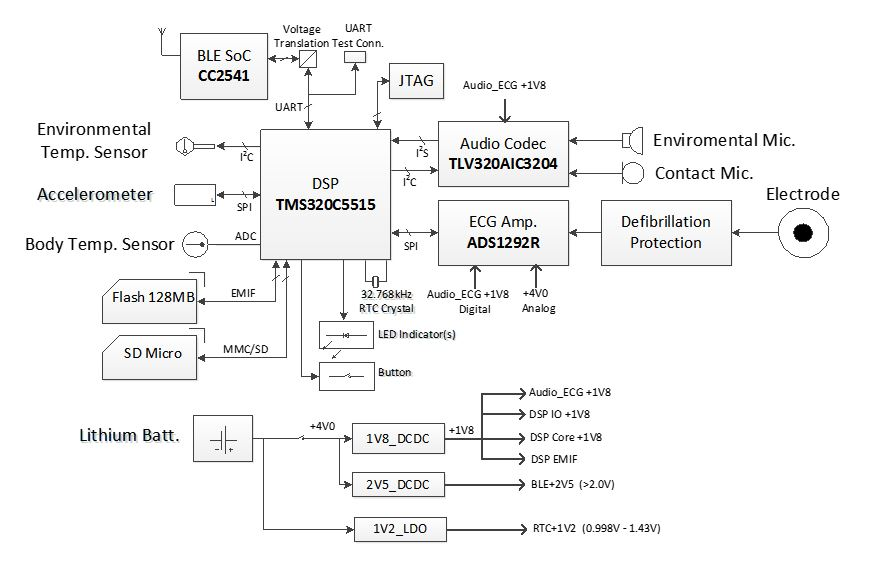
\includegraphics[scale = 0.75 ]{BlueBox_Architecture.JPG}
	\caption{BlueBox Hardware System Architecture\label{BlueBox_Architecture}}
\end{figure} 


\begin{figure}[h]
	\centering
	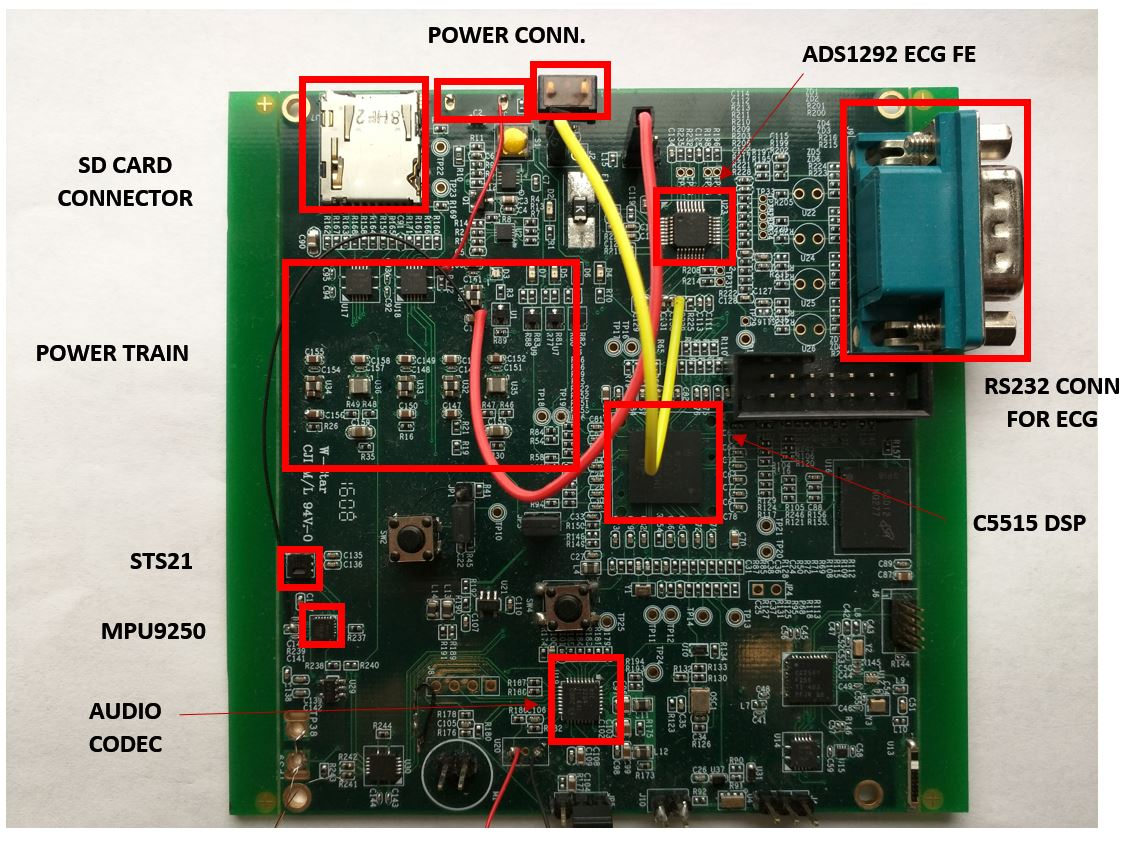
\includegraphics[scale = 0.5]{BlueBox_Hardware.jpg}
	\caption{BlueBox Prototype Hardware \label{BlueBox_Hardware}}
\end{figure} 
\section{Digital Signal Processor}
TMS320C5515 is a fixed-point DSP based on the TMS320C55x™ CPU processor core. The C55x\textsuperscript{TM} DSP architecture achieves high performance and low power through increased parallelism and total focus on power savings. Figure \ref{C5515 Architecture} shows the DSP architecture.

\begin{figure}[h]
	\centering
	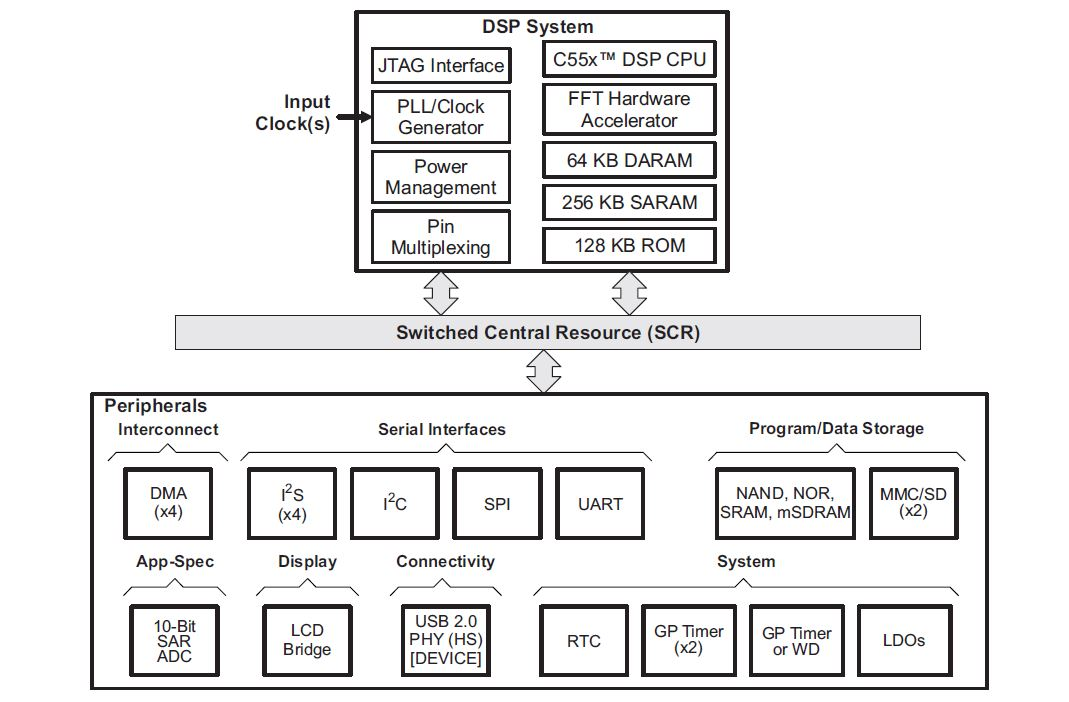
\includegraphics[scale = 0.75 ]{C5515_arch.JPG}
	\caption{DSP Architecture. \cite{tms320c5515}\label{C5515 Architecture}}
\end{figure} 
\subsection{Clock Frequency}The DSP has a low power software programmable Phase Locked Loop (PLL) clock generator that supports 60-, 75-, 100-, 120-MHz clock rate.
\subsection{On-Chip Memory}The DSP has 320K Bytes Zero-Wait state On-Chip RAM and 128K of On-Chip ROM. 

\subsection{Peripherals} The DSP has general-purpose input and output functions along with the 10-bit Successive approximation register (SAR) Analog to Digital converter ( ADC) provide sufficient pins for status, interrupts, and bit I/O for LCD displays, keyboards, and media interfaces. Serial media is supported through two Multimedia Card/Secure Digital (MMC/SD) peripherals, four Inter-IC Sound (I2S Bus™) modules, one Serial-Port Interface (SPI) with up to 4 chip selects, one I2C multi-master and slave interface, and a Universal Asynchronous Receiver/Transmitter (UART) interface. 

\subsection{DMA} The device includes four Direct Memory Access (DMA) controllers, each with 4 channels, providing data movement for 16-independent channel contexts without CPU intervention. Each DMA controller can perform one 32-bit data transfer per cycle, in parallel and independent of the CPU activity.


\subsection{Power} Furthermore, the device includes three integrated low-dropout (LDO) regulators (DSP LDO, ANA LDO, and USB LDO) to power different sections of the device. The DSP LDO can provide 1.3 V or 1.05 V to the DSP core (CVDD), selectable on-the-fly by software as long as operating frequency ranges are observed. 


\section{AIC3204 : Audio Codec}
TLV320AIC3204 is an analog interface chip (AIC) of Texas Instruments which is a flexible, low-power, low-voltage stereo audio codec with programmable inputs and outputs, PowerTune capabilities, fixed predefined and parameterizable signal-processing blocks, integrated PLL, integrated LDOs and flexible digital interfaces. It has both recording and playback capabilities. The record part of the TLV320AIC3204 covers operations from 8kHz mono to 192kHz stereo recording, and contains programmable input channel configurations covering single-ended and differential setups, as well as floating or mixing input signals. It also includes a digitally-controlled stereo microphone preamplifier and integrated microphone bias. It integrates A / D and D / A conversion functions, it achieved high-precision A / D and D / A converter in the low-cost using $\Sigma$-$\Delta$ technology. The size of the chip is very small and compact and its is available in 5 mm × 5 mm 32-pin QFN Package. 

\begin{figure}[h]
	\centering
	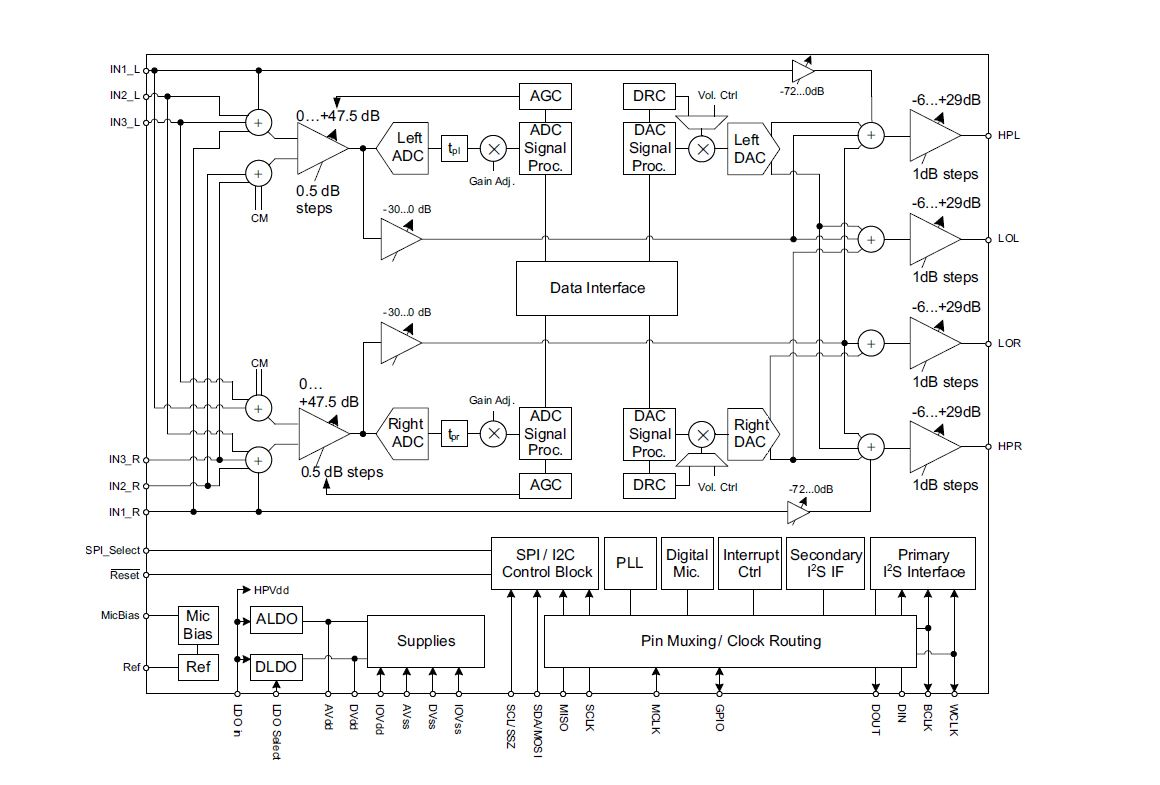
\includegraphics[scale = 0.7 ]{AIC3204.JPG}
	\caption{AIC3204 Block Diagram. \cite{audiocodec}\label{aic3204}}
\end{figure}

Figure \ref{aic3204} displays the audio codec's architecture. It has capabilities of recording stereo audio signals. It has two channels that it can record. One channel is used for respiration recording and the other for paramedic's log recording. Each channel of the stereo audio ADC consists of a signal-processing engine with fixed processing blocks. The signal processing blocks available are: First-order Infinite Impulse Response (IIR), Scalable number of biquad filters, Variable-tap Finite Impulse Response (FIR) filter and Automatic Gain Control (AGC). The choice between these processing blocks is part of the PowerTune strategy to balance power conservation and signal-processing flexibility. Less signal-processing capability reduces the power
consumed by the device.
\section{ADS1292R : ECG Frontend}
ADS1292R is the ECG analog front end chip to which the electrode output is connected to. ADS1292R is a two channel, simultaneous sampling, 24-bit, delta-sigma ($\Delta$$\Sigma$) analog-to-digital converters (ADCs) with a built-in programmable gain amplifier (PGA), internal reference, and an on-board oscillator. ADS1292R incorporate all features commonly required in portable, low-power medical electrocardiogram (ECG), sports, and fitness applications. With high levels of integration and exceptional performance, the ADS1292R enable the creation of scalable medical instrumentation systems at significantly reduced size, power, and overall cost. ADS1292R have a flexible input multiplexer per channel that can be independently connected to the internally-generated signals for test, temperature, and lead-off detection. Additionally, any configuration of input channels can be selected for derivation of the right leg drive (RLD) output signal. The ADS1292R operate at data rates from 500SPS up to 8 kSPS. The devices are packaged in a 5-mm × 5-mm, 32-pin thin quad flat pack (TQFP). Operating temperature is specified from –40°C to +85°C. ADS1292R is interfaced with the DSP through SPI.
 \begin{figure}[h]
 	\centering
 	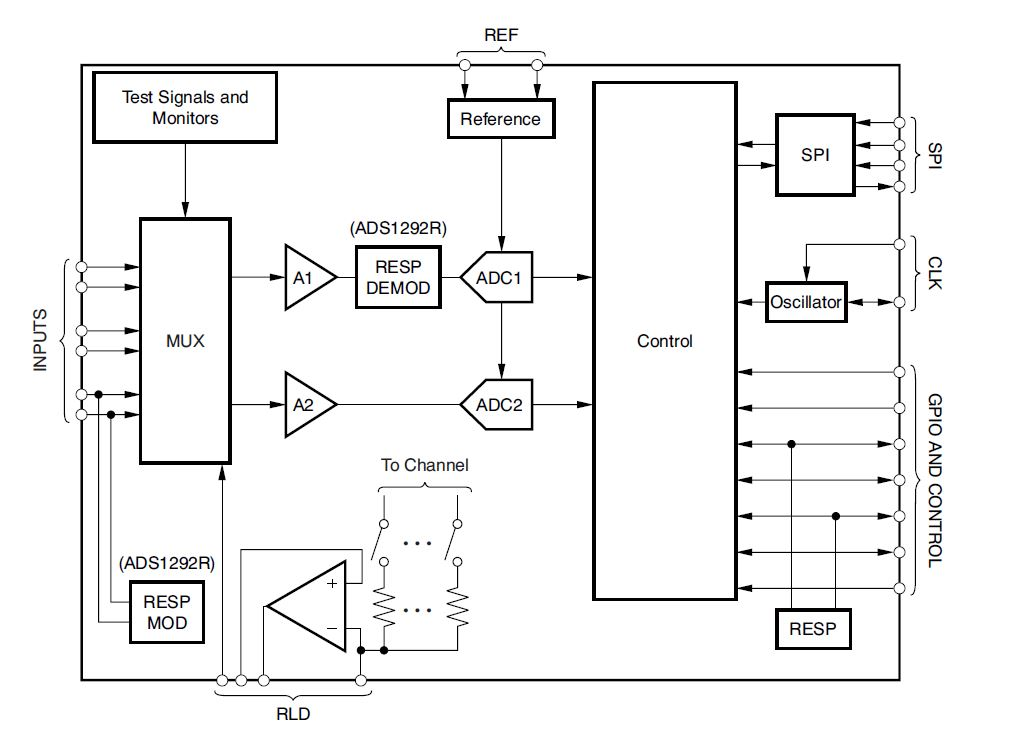
\includegraphics[scale = 0.7 ]{ADS1292R.JPG}
 	\caption{ADS1292R Functional Block Diagram. \cite{ads}\label{ADS1292R}}
 \end{figure}
 
\section{MPU9250 : Accelerometer sensor}\label{mpu9250_def}
MPU-9250 is a 9-axis MotionTracking device that combines a 3-axis gyroscope, 3-axis accelerometer, 3-axis magnetometer and a Digital Motion Processor\textsuperscript{TM} (DMP). With its dedicated I2C sensor bus, the MPU-9250 directly provides complete 9-axis MotionFusion\textsuperscript{TM} output. MPU-9250 features three dedicated 16-bit analog-to-digital converters (ADCs) for digitizing each of the gyroscope outputs, accelerometer outputs, and magnetometer outputs. For precision tracking of both fast and slow motions MPU-9250 provides a user-programmable accelerometer full-scale range of ±2g, ±4g, ±8g, and ±16g. The package size down to a footprint and thickness of 3x3x1mm, to provide a very small yet high performance low cost package. The following figure shows the architecture of MPU9250.A valid accelerometer datat is available 30 ms(typical) after wakeup from sleep.
\begin{figure}[h]
	\centering
	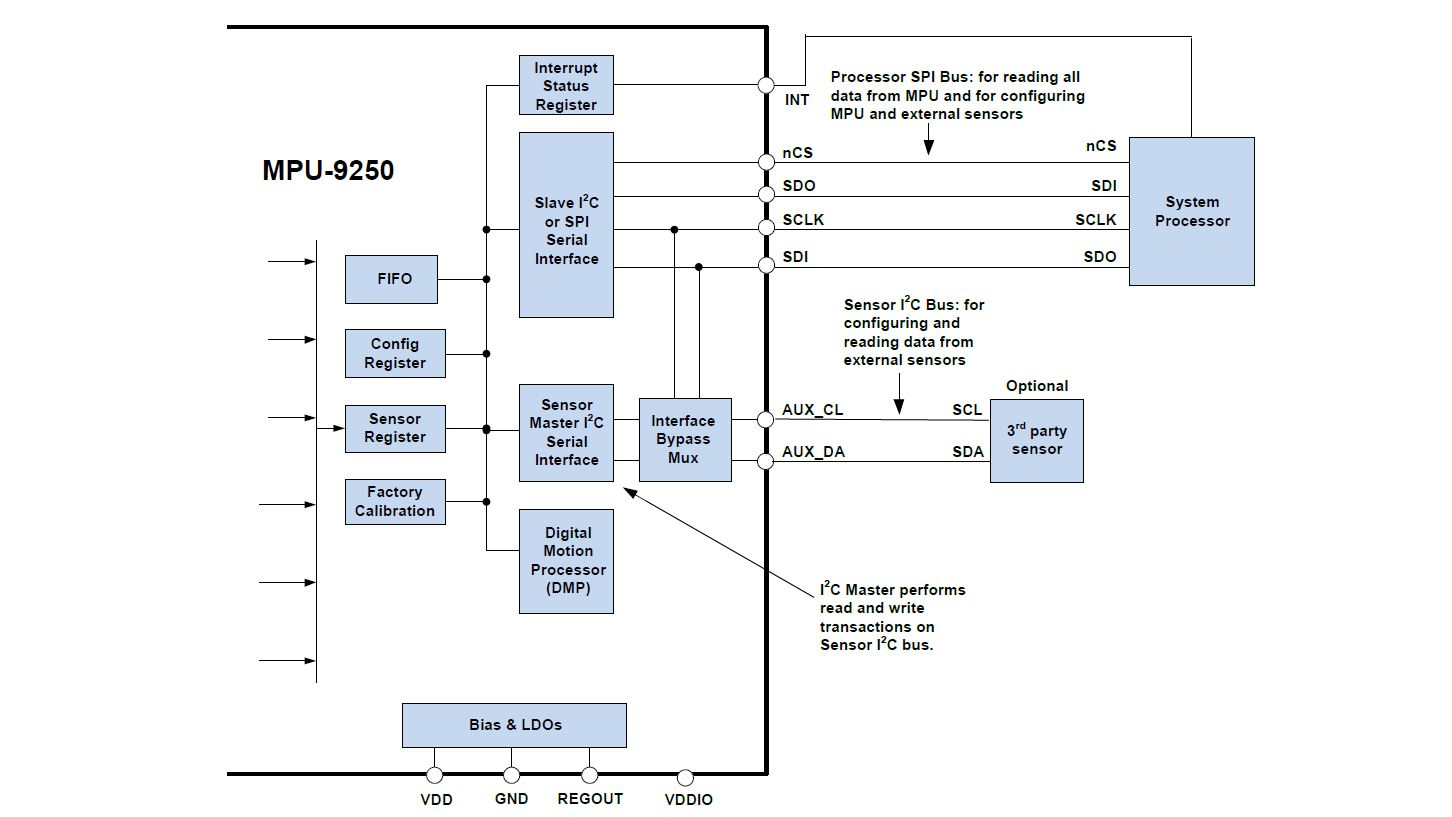
\includegraphics[scale = 0.6]{MPU9250.JPG}
	\caption{MPU9250 Architecture. \cite{mpu}\label{mpu9250}}
\end{figure}

The MPU-9250 contains a 512-byte FIFO register that is accessible via the Serial Interface. The FIFO configuration register determines which data is written into the FIFO. Possible choices include gyro data, accelerometer data, temperature readings, auxiliary sensor readings, and FSYNC input. A FIFO counter keeps track of how many bytes of valid data are contained in the FIFO. The FIFO register supports burst reads. The interrupt function may be used to determine when new data is available. 

The MPU9250 has multiple user-configurable power modes. The mode which we are interested is Sleep mode (consumes 8 $\mu$A)and Low-Power Accelerometer Mode which consumes 450 $\mu$A. 
 
\section{Temperature sensor}
\subsection{ STS21 : Environment temperature sensor}
STS21 is a low power, fully self calibrated digital temperature sensor well suited for applications with high demand on temperature accuracy. With dedicated I2C bus it directly provides the temperature output. The sensor comes in a package sized 3 x 3mm footprint and 1.1 mm height. The sensor is powered up to the chosen supply voltage VDD (between 2.1V and 3.6V). After power-up, the sensor needs at most 15ms for reaching idle state, i.e. to be ready accepting commands from the DSP. Current consumption during start up is 350$\mu$A maximum. Whenever the sensor is powered up, but not performing a measurement or communicating, it is automatically in sleep mode (idle state). STS21 measures temperature with different resolution ranging from 14 bits to 11 bits, where the 14 bit resolution takes 85ms for conversion whereas a 11 bit resolution takes somewhere between 9 and 11 ms.

\subsection{MA100: Body temperature sensor} 
MA100 is a Biomedical Chip Thermistor assemblies that are designed for use in applications involving both intermittent and continuous patient temperature monitoring. Although low in cost and small in size, these are highly stable, precision thermochips provide reliability, tight interchangeable tolerances, geometries, and fast response time that are often required.
 
\section{Memory}\label{memory}
The BlueBox system has on-chip memory and the persistent micro SDHC(secure digital high capacity) card storage. Because a micro SD card is power intensive and takes hundreds of milliseconds to write to, the on-chip memory is used as buffer. Once there is enough data in the buffer it is written to the SD card and can be accessed by a computer. All the heavy lifting data transfer are done with the help of Direct Memory access(DMA) peripheral interconnect to take off load from DSP. SD card is interfaced to DSP using MMC/SD interface. The SD card used for the application is a high capacity card that can support a maximum clock frequency of 50 MHz. These high capacity cards are not byte addressable. They are organized in 512 Byte sector or block and thus are block addressable. BlueBox uses kingston 8 GB micro SDHC card. the SDHC card is very power hungry. It consumes 150 mA when operated at 50 MHz during active read/write operation and consumes 30 mA during inactive periods.

\section{Battery and Power management circuitry}
 A GMB 302547 Lithium ion polymer rechargable battery, shown in figure \ref{fig:battery} is used to power the system. It has a capacity of 300 mAH at 3.7 V. It is 4 cm long, 2cm wide and 0.2 mm thick. And it weighs 8 grams. The battery is place on top of the central board housing. The central board has a battery charging circuitry that can charge the battery completely in 2 hours. The power management circuitry provides a power-train that feeds the different power domain of the DSP as shown figure \ref{BlueBox_Architecture}.
 \begin{figure}[h]
 	\centering
 	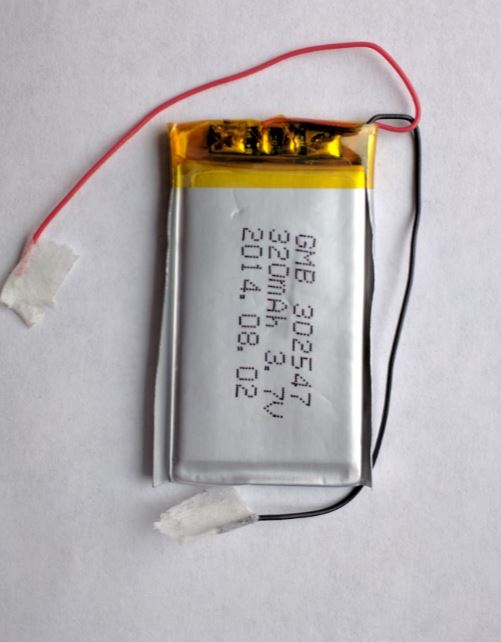
\includegraphics[scale = 0.25 ]{battery.JPG}
 	\caption{Lithium Polymer battery}\label{fig:battery}
 \end{figure}      

\nomenclature{PLL}{ Phase Locked Loop }
\nomenclature{SAR}{ Successive Approximation Register }
\nomenclature{ADC}{ Analog to Digital Converter } 
\nomenclature{I2C}{ Inter Integrated Circuit } 
\nomenclature{I2S}{ Inter-IC Sound } 
\nomenclature{SPI}{ Serial Peripheral Interface }
\nomenclature{UART}{ (Universal Asynchronous Receiver/Transmitter }
\nomenclature{MMC}{ Multi Media Card }
\nomenclature{DMA}{ Direct Memory Access }
\nomenclature{LDO}{ Low DropOut }
\nomenclature{USB}{ Universal Serial Bus }
\nomenclature{RTC}{ Real-Time Clock }
\nomenclature{AIC}{ Analog Interface Chip }
\nomenclature{AGC}{ Automatic Gain Control }
\nomenclature{FIR}{ Finite Impulse  Response }
\nomenclature{IIR}{ Infinite Impulse  Response }

%%% Local Variables: ***
%%% mode: latex ***
%%% TeX-master: "thesis.tex" ***
%%% End: ***

\chapter{Firmware Architecture}

Chapter 4 explains the firmware architecture of the BlueBox system and describes its core functionalities. This chapter also talks about procedure for importing and visualizing the acquired data.

\section{Overview}
The firmware for the system is implemented on Texas Instrument's TMS320C5515 DSP in C and assembly using Code Composer Studio IDE. TI provides DSP/BIOS (in later versions called SYS/BIOS)  a real time operating system for their DSPs. These operating systems provides a wide range of system services to an embedded application such as preemptive multitasking, memory management and real-time analysis. The RTOS is feature rich and helps in quicker development and testing of firmware. But the very important of drawback of using the RTOS is the trade off of performance and controllability of the DSP for quicker development. For a resource and power constrained application, it is required to squeeze out the performance from the system which requires the firmware to have complete control over the underlying hardware. Thus firmware for the system is implemented on baremetal using  C and using the chip support library (CSL) for C5515 provided by TI. 


\vfill

The functions of Software could be categorized as the following:
 \begin{description}
 	\item[$\bullet$]
Initializing System and Sensors 
 	\item[$\bullet$]
Data collection and storage
 	\item[$\bullet$]  
Power management 
 \end{description}

 \begin{figure}[h]
	\centering
	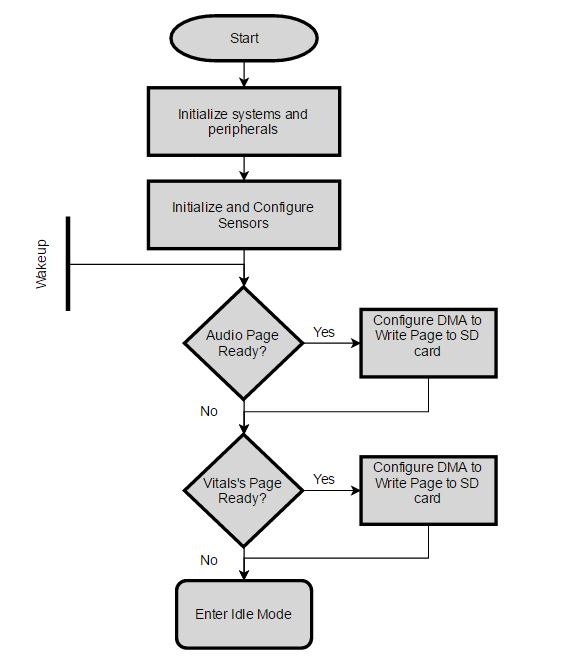
\includegraphics[scale = 1 ]{main.JPG}
	\caption{Main thread\label{main}}
\end{figure}

 \begin{figure}[h]
	\centering
	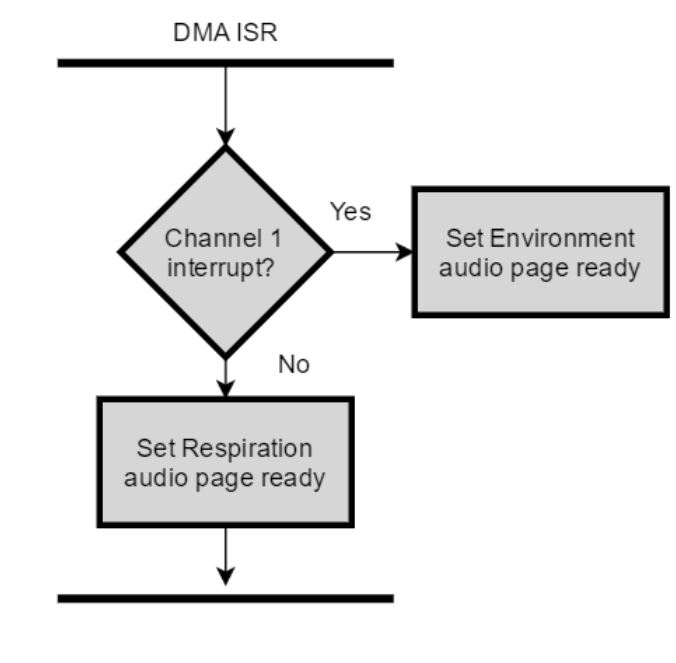
\includegraphics[scale = 0.5 ]{dma_interrupt.JPG}
	\caption{DMA Interrupt Service Routine\label{dma_isr}}
\end{figure}

 \begin{figure}[h]
	\centering
	\includegraphics[scale = 1 ]{ECG_interrupt.JPG}
	\caption{Hardware Interrupt Service Routine\label{ecg_isr}}
\end{figure}

\section{Initializing System}
First thing the firmware does after boot-up is to initialize the clock by configuring the PLL registers. PLL is configured to generate a 100 MHz clock to tick the system. After the clocks have been set up, the multiplexed I/O pins are configured to function as a specific peripheral or a input/output pins. Then the clock and power to those I/O pins and peripherals are enabled. After the I/O pins are configured, the communication peripherals such as SPI,I2C and I2S are configured. Their mode of operation(master or slave) , frequency of operation etc are initialized and configured. DSP's I2S module is configured as the I2S master(who supply bit clock and word clock) and the Audio codec AIC3204 is configured as the I2S slave. 

\section{Initializing sensor}
Audio Codec AIC3204 is configured, through the I2C interface , to sample the audio signal at 12Khz on each of the two channels and configured to amplify the signal with automatic gain correction feature enabled. The codec is also configured to filter the audio signal using first order IIR filter and 5 BiQuad filters to improve the audio quality. 

The ECG analog front end ADS1292R is configured to sample ECG signal at 500 samples per second. ADS1292R is configured to generate a hardware interrupt to inform the DSP when the sample is ready so that DSP can read the data using SPI interface. The ECG data is again stored in a ping-pong buffer and the data is stored in the permanent storage with the same mechanism as mentioned earlier. 
The environment temperature sensor STS21 is configured to sample the temperature with a 11bit precision. This data is acquired by polling. For every 500 ECG interrupt the STS21 is polled once to collect the temperature data.  
The Analog to Digital converters on board are configured to  sample the body temperature once for every 500 interrupt of ECG.

\section{Data Collection and storage}
The firmware is designed for concurrent data acquisition using dedicated hardware resources for the signals of interest. These hardware resources can perform certain required but  very defined functionalities like data buffering, filtering and data moving  without the intervention of the DSP. These hardware accelerators requires the DSP to configure for them to operate. The designed firmware is primarily preemption based where the DSP configures, assigns work, to the peripherals and hardware accelerators to concurrently acquire the signals.Upon completion of the assigned work , I.e data acquisition, these accelerators interrupt the DSP and the DSP configures DMA to write the collected data into the SD card. These sequence of interrupts and services happens periodically to acquire and store the signals.


\hspace{10mm} There are two non-mask able interrupts that preempts the DSP. One is the DMA interrupt, generated upon acquisition of audio signal of preconfigured size  and other one is the hardware interrupt generated by the ECG frontend signaling that the ECG data is ready. The following flow chard gives the functionality of DMA ISR and the hardware interrupt ISR.The ECG ISR is responsible of acquiring the available ECG data from the front end and also for acquiring the body and the environment temperature and accelerometer data.
 
 The following would provide insight and explain in detail the above mentioned mechanism with the context of audio signal acquisition .There are primarily two audio channels that are sampled at a very high frequency of 12 KHz. The audio signal acquisition and storage is the most intensive task of the entire system and also very power hungry task. Involving DSP to do the complete task would completely utilize the DSP's computational bandwidth allowing no space for DSP to do other useful work and also the overhead of doing this operation through DSP is very high.  TMS320C5515 includes 4 DMA controllers with four DMA channels each. It can move data among internal memory, external memory, and peripherals without intervention from the DSP and in the background of DSP operation. So DMA data transfer is used in audio signal collection and storing.  The following diagram shows the DMA in the DSP 
 \begin{figure}[h]
 	\centering
 	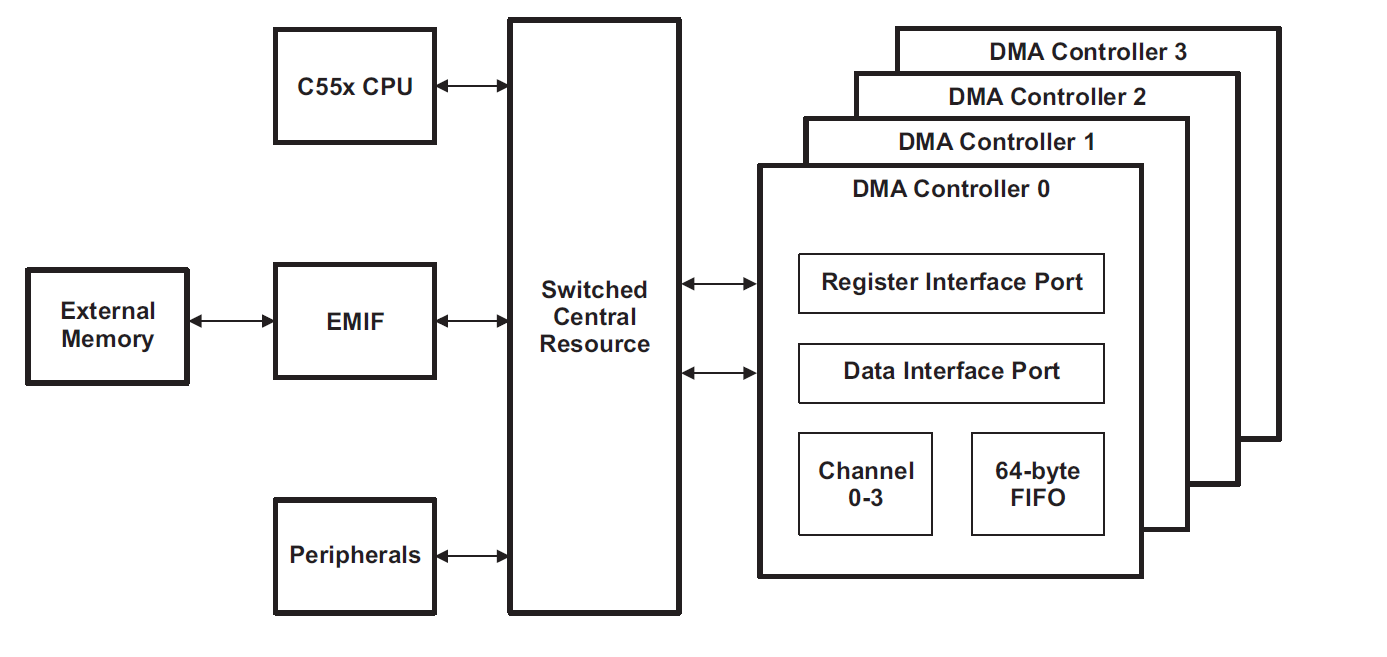
\includegraphics[scale = 0.5 ]{DMA_overview.PNG}
 	\caption{Conceptual Block Diagram of DMA controller\label{DMA_Architecture}}
 \end{figure} 
 The DMA is configured to collect the audio signal from the I2S peripheral and move it to SD card.The I2S receive event triggers the DMA to collect the audio signal. When the DMA fills up the allocated buffer it interrupts the CPU and the DSP initiates the SD card write using  other DMA channels and DMA takes care of the further action. The system continues acquiring audio signals even while writing data into the SD card . This is done through using DMA in ping-pong mode. The following diagram shows the ping pong operation mode.
  \begin{figure}[h]
 	\centering
 	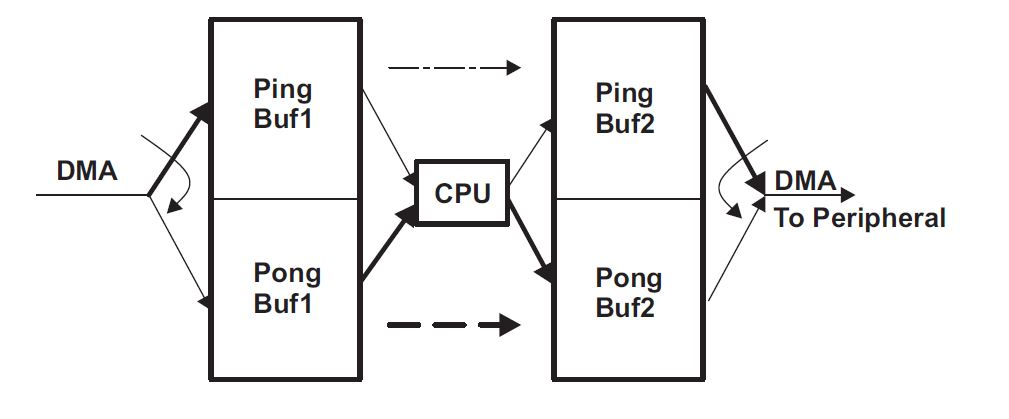
\includegraphics[scale = 0.5 ]{ping_pong.JPG}
 	\caption{Ping-Pong Mode for DMA Data Transfer\label{ping_pong}}
 \end{figure}
 When the ping buffer data is being copied to the SD card , the DMA acquires the incoming data and fills it in the pong buffer. So DMA used in ping-pong mode enables the system to collect the audio signals and store the previously cached signal simultaneously. 
 
 As mentioned earlier the measurement of temperature signal is triggered for every 500 interrupts of ECG. This adds a overhead of checking if the interrupt count every time ECG interrupt is serviced. The measurement of temperature from the context of ECG interrupt increases the worst case execution time of the ISR which is not preferred in general for typical application. One could argue that the system could have used a timer and generate a timer interrupt every one second and trigger the temperature measurement instead of tightly coupling it with the ECG ISR. The reason for not going with this approach is the cost in terms of power for running a dedicated timer for the temperature measurement. Power is the most scarce resource in the system and that is the important reason why the former method is chosen than the latter one. As long as the tasks could be finished on available clock cycles without disturbing other functionality of the system, it is fine even if the worst case execution time of the ISR increases.
 \begin{figure}[h]
 	\centering
 	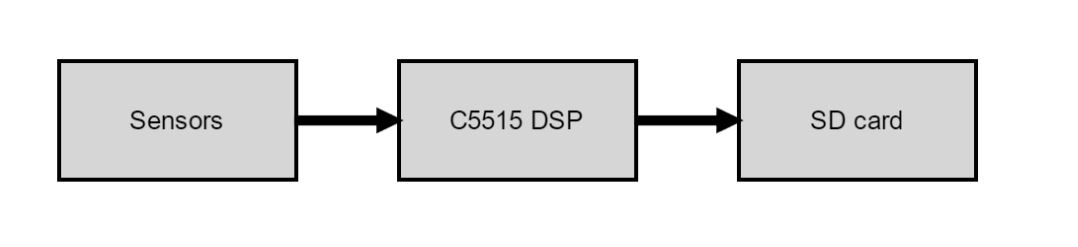
\includegraphics[scale = 0.5 ]{record_dataflow.JPG}
 	\caption{Flow of data in during record\label{record_datalow}}
 \end{figure}

\subsection{Importing the Data}
Once the data has been saved to the micro SD card and testing is complete, it can be read directly by a computer. A custom file system is used to store the data, so it can not be directly recognized on a computer. A filesystem driver for the custom filesystem is developed in python, which could parse the data in the SD card and create files of each of the signals. These files are read by a MATLAB script that does post processing and generates data vectors corresponding to each signal. For example in case of body temperature sensor, the data in the file is the raw ADC values, the calibration details of the body temperature is embedded into MATLAB code , so it does convert raw ADC temperature  data into a meaningful value through the calibration information.  
MATLAB plots the data and visualizes it in such a way that the user can relate and see all the signals together and it allows user to jump into the time of interest. 
 \begin{figure}[h]
	\centering
	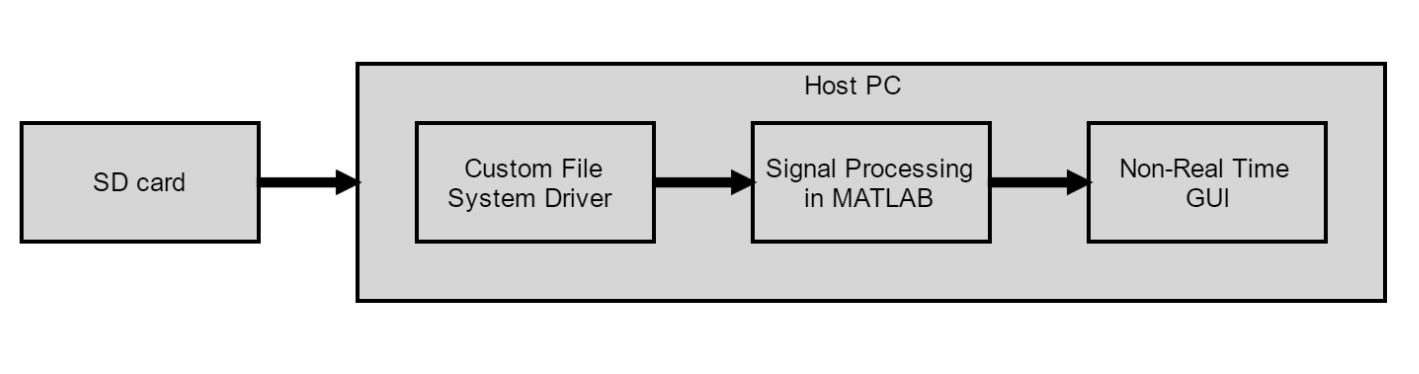
\includegraphics[scale = 0.5 ]{play_dataflow.JPG}
	\caption{Flow of data in import record\label{play_dataflow}}
\end{figure}

\\TODO MATLAB GUI screenshot

\chapter{Low-Power Firmware Design Techniques}

Chapter 5 gives a background on general sources of power consumption in a digital system and describes some of the primitive techniques used for power management. Section 5.4 describes the design flow of power management techniques for BlueBox system. Section 5.5 to 5.7 explains the details of those techniques.  
\section{Background} In order to design successfully for low power consumption, it is important to have a through understanding of the sources  of power dissipation, the factors that affect them and the methodologies and techniques that are available to achieve optimal results.  
Throughout this chapter, we discuss power consumption and methods for reducing it. Energy is the time integral of power; if power consumption is a constant, energy 
consumption is simply power multiplied by the time during which it is consumed. 
Reducing power consumption only saves energy if the time required to accomplish the 
task does not increase too much.The chapter presents the sources of power dissipation and describes the important low-power methodologies and power optimization techniques available. Low-power design can be applied on various abstracted levels, such as system level, architectural level and technological level. This chapter could as well be utilized as a quick review on low power design. 

\section{Sources of power consumption}\label{src_pwr}
Most components are currently fabricated using CMOS technology\cite{cypress,silicon}. Main reason for this bias is that CMOS technology is cost efficient and inherently lower power than other technologies. So the sources of power consumption talked in this chapter is based on CMOS component model. There are a number of sources of power consumption in CMOS, which can be subdivided into \textit{static} and \textit{dynamic} power dissipation. The main difference between them is that dynamic power is frequency dependent, while static is not. Dynamic power dissipation is primarily caused by the switching of the CMOS devices (MOSFETs) when logic values are changed (known as \textit{capacitive power} or \textit{switching power}). The amount of power that is dissipated is directly related to the switching activity (which is the number of logic transitions per clock cycle in the entire circuit), the clock frequency, the supply voltage, and the capacitive load the circuit drives \cite{PowerAwareDesign}. Another source of dynamic power dissipation is \textit{short-circuit power}. CMOS is comprised of both PMOS and NMOS devices. During a logic transition, the PMOS and NMOS devices are simultaneously turned on for a very short period of time, allowing a short-circuit current to run from V\textsubscript{dd} to ground\cite{Low-powercmos,LowPowerDesign}. This behavior is inherent to CMOS switching.The more dominant component of dynamic power is capacitive power. This component is the result of charging and discharging parasitic capacitances in the circuit. Every time a capacitive node switches from ground to V\textsubscript{dd} an vice-versa energy is consumed. 

Static power, which is a constant factor and has nothing to do with the switching activity, is caused by \textit{leakage power}. In an ideal situation, a static CMOS circuit (i.e. one that does not switch) does not consume any power because there is no direct path from V\textsubscript{dd} to 
ground. In real life there will always be leakage currents, since CMOS devices are not 
perfect switches. The total power dissipation can be described by the following formula:
\[P_{total} = \alpha(C_L . V_{DD}^2.f_{clk}) + I_{sc}. V_{DD} + I_{leak} . V_{DD}    \hspace{10mm} (1) \]

The Greek letter $\alpha$ represents the \textit{switching activity} in the circuit, expressed in a value between 0 (no switching activity at all) to 1(maximum switching activity). C\textsubscript{L} is the capacitive load, driven by the circuit. As can been seen in the formula, the dynamic
power consumption depends on V\textsubscript{dd} square, which makes the supply voltage a very
important factor in low-power design, as will be explained later. I\textsubscript{SC} and I\textsubscript{leak} represent
the total short circuit and leakage current, respectively.It is important to realize that
that I\textsubscript{SC} is a variable, while I\textsubscript{leak} is not. I\textsubscript{SC} depends on the charge carried by the
short-circuit per transition, the cycle time, and the total number of transitions
\[I_{SC} = Q_{SC}  \cdot  f \cdot \alpha    \hspace{10mm} (2) \] 

A better way to represent the formula would be like this:

\[P_{total} = \alpha(C_L \cdot V_{DD}^2 \cdot f_{clk}) +  Q_{SC}  \cdot  f_{clk} \cdot V_{DD} + I_{leak} \cdot V_{DD}    \hspace{10mm} (3) \]
It is a misunderstanding that reducing power consumption will always lead to a
reduction in energy as well. When we refer to power, we refer to the momentary
electric energy that is dissipated, measured in Watts. Energy is measured in Joules, or Watts per second. Thus, the energy consumption depends on the power consumption and the time it takes to perform a task. For example, if we have two circuits A and B, and P\textsubscript{A} = 2P\textsubscript{B}, and 2D\textsubscript{A} = D\textsubscript{B} (where ’D’ refers to the delay of the circuits), then EA = EB. Thus, even though the power consumption of circuit B is twice as low as circuit A’s, no energy is saved. When we take another look at formula (3) , reducing $\alpha$ , V\textsubscript{DD}, and C\textsubscript{L} will always reduce power and energy consumption. Lowering f\textsubscript{clk} reduces
only power, not energy \cite{PowerAwareArchitecting}.

\section{Basic Low-Power Design Methodologies}
 The following methodologies are most powerful ones and are the most basic ones for any system. They include voltage scaling, frequency scaling , clock gating and power gating. All these methodologies helps to reduce the power consumption but comes at a cost. For example frequency scaling could affect the execution time of the application , power gating causes a boot up latency whenever the system or peripheral needs to be powered on. It purely depends on the application requirement to decide on the tradeoff. If the application can tolerate the cost of a methodology , then it can be used to reduce the power consumption. So , the BlueBox system adopts a few of these basic methodologies but not all of those. It is still important to have a basic idea of these basic methodologies and the insight they provide on power consumption. 
 
 \subsection{Static voltage scaling}
 One way to decrease the power consumption significantly, is to decrease the supply 
 Voltage. As mentioned in the previous section \ref{src_pwr},  dynamic power consumption depends quadratically 
 on V\textsubscript{DD}. Voltage scaling is therefore the most effective method to limit the power 
 consumption. However, when V\textsubscript{DD} is lowered, it comes at a price: the delay of the logic 
 increases. In systems where we desire a high throughput, and ask for the maximum 
 performance of the technology being utilized, voltage scaling is not an option. If V\textsubscript{DD} 
 would be lowered, we would not be able to meet the performance requirements. In many 
 situations however, we do not ask for the maximum performance and we can safely lower 
V\textsubscript{DD} in order to save power. Even though delay is increasing, the power-delay product 
 is improving when V\textsubscript{DD} is decreased, since power decreases quadratically while delay 
 increases less fast. Delay scales with:
 \[ \frac{V_{DD}}{
 	(V_{DD} - V_{TH})^2
 	} \hspace{20mm}(4)\]     
 
 \subsection{Dynamic voltage scaling}
 Instead of a fixed supply voltage during circuit operation it is also possible to dynamically 
 adjust the supply voltage based on the current required performance of the circuit. The 
 required performance is often not always the same. When the required performance 
 of the circuit is momentarily reduced, we can afford lower supply voltages. This is 
 called dynamic voltage scaling (DVS). Apart from lowering the supply 
 voltage, it is also possible to lower the clock frequency. A reduction in V\textsubscript{DD} will always 
 increase the delay to some extent, but if the cycle time is still much higher than the delay 
 of the circuit, energy is wasted. Therefore dynamic voltage and frequency scaling 
 (DVFS) can be employed to save energy to the maximum.
 
 \subsection{Frequency Scaling}
 Apart from V\textsubscript{DD}, there is another variable in the equation of section \ref{src_pwr} that intuitively 
 suggests possibilities for reducing power: frequency. Of course, the clock frequency is 
 bound by the desired throughput of the system. However, a system does rarely operate at 
 its maximum throughput all the time. Often, the desired throughput is much lower than 
 its maximum performance. Then, it is possible to lower the operating frequency in order 
 to save power (and thus also energy), which is called frequency scaling. Sometimes 
 voltage scaling and frequency scaling are employed simultaneously, such as in cell phones, 
 when they are in stand-by mode.
 
 \subsection{Clock gating}
 In the previous sections we have referred to (sub)systems that do not always operate 
 at their maximum performance. It is also possible that parts of a system are idle for a 
 period of time: then no useful computational work is performed. Still, there is power 
 consumed. A subsystem being idle does not necessarily mean that the subsystem is not 
 performing any computations. It only means that the results are not being utilized. This 
 is possible when the subsystem is still fed with data, but the result is discarded, because 
 it is not needed at that moment. But even when the subsystem is not performing 
 any computational work, there is still the static power dissipation (leakage power) of 
 the subsystem. What is more, flip-flops dissipate some dynamic power every single clock 
 cycle, even when the in- and outputs remain the same. If there are large registers present 
 in these subsystems, this power dissipation can become quite significant. And, finally, 
 there is the power dissipation of the clock network in the subsystem. Clock networks 
 are very expensive in terms of power. A major portion of the total power consumption 
 of the system is dissipated in the clock network (mainly in the clock buffers/drivers) \cite{LowPowerMethod}. 
 Considering the above, there is a lot of power that can be saved when a subsystem 
 is idle. One way to achieve this goal is to apply clock gating. This essentially means 
 that the clock signal of the subsystem is cut off. This will save the power dissipated in 
 flip-flops and the clock network. If the combinational logic in the subsystem is fed by 
 registers at the inputs, the logic will stop switching \cite{DesignLowPower}. It will, however, not save the 
 leakage power.
 
 \subsection{Power Gating}
 Power gating provides basically a solution to the same problem mentioned in clock gating section.Power gating has however an important advantage over clock gating: it is capable 
 to save static power of idle blocks as well, since it cuts of the power supply instead of 
 the clock signal. In order to do that, blocks need to be placed onto separate ”power 
 domains”, which can be powered on and off. 
 When a block is asleep it costs some time to wake it up again, the same as it costs 
 some time to put a block to sleep. This introduces additional delays. Also during 
 wake-up and going to sleep, still some leakage power is dissipated which makes power 
 gating not perfect. There is always a cost associated with the state transition.The essential criteria for implementing power gating is the total leakage power component and how many and how often blocks are idle. The leakage power highly depends on the technology being utilized and the impact of the leakage 
 power highly depends on the system frequency being utilized. If the leakage component 
 is significant and many blocks are idle for longer periods of time, power gating may 
 be efficient. One should however be aware of the fact that power gating is much more 
 difficult to implement than clock gating and leads to significantly higher costs (mainly 
 because of all the switches that are required). It is also important to realize that power 
 gating is much more invasive than clock gating. While clock gating does not affect the 
 functionality of the system, power gating does. It affects inter-block communication and, 
 as mentioned before, adds time delays to safely enter and exit power gated modes \cite{LowPowerMethod}. 
 
 \section{Design flow}
 
 Design flow of any system constitutes of various level of abstraction. Abstraction reduces complexity  and allow efficient design and implementation of complex systems.The aspect of the system that needs to be optimized helps in designing the various levels of abstraction. When a system is designed with the emphasis on power optimization , then the design must embody optimization at all levels of the design flow. In general the support for energy management needs to be incorporated at the system level and the architectural level. An important aspect of the design flow is the relation and feedback between the levels. Paul J.M Havinga et. al, 
 have come up with three layers of abstraction: system, architecture and technology \cite{havinga,havinga2,havinga3}. Figure \ref{fig:quote} describes the abstraction level and related examples for energy reduction.
 \begin{table}
 	\centering
 	\begin{tabular}{|l|l|}
 		\hline
 		$Abstraction level$ & $Examples$  \\
 		\hline
 		  & processing method \\
 		  & energy manager \\
 		  system & scheduling \\
 		  & light weight filesystem \\
 		  & system partitioning \\
 		  & parallel hardware \\
 		  architecture & Direct Memory Access \\
 		  & FFT hardware \\
 		  & compiler \\
 		  & clock gating \\
 		  technological & clock frequency control \\
 		  & voltage control \\
 		\hline
 	\end{tabular}
 	\caption{Abstraction level and related example for energy reduction.}
 	\label{table:abstraction}
 \end{table}


 At the highest level the design decisions have the most influence. 
 Therefore, the most effective design decisions derive from choosing and optimizing 
 architectures and algorithms at the highest levels. It has been demonstrated by several 
 researchers [63] that system and architecture level design decisions can have dramatic 
 impact on power consumption. However, when designing a system it is a problem to 
 predict the consequences and effectiveness of high level design decisions because implementation details can only be accurately modelled or estimated at the technological 
 level and not at the higher levels of abstraction. Furthermore, the specific energy 
 reduction techniques that are offered by the lower layers can be most effective only 
 when the higher levels are aware of these techniques, know how to use them, and apply 
 them.
 
 
 The above mentioned layers can be considered as vertical layers of any digital system. The BlueBox system could be broken down into three main subsystem as shown in figure \ref{table:sub-system} based on its application semantics: sensor, processor and storage subsystem.These sub-systems work together and are interdependent on each other for their functionalities. Each of these subsystem contains  all three abstraction layers mentioned above. Our low-power design flow targets each of these three horizontal layers of subsystem individually and the interdependent  vertical layers within them. It is interesting that effect on a single subsystem creates space for further power savings for its dependent subsystem. 
 
  \begin{table}
 	\centering
 	\begin{tabular}{|l|l|}
 		\hline
 		$Sub$-$System$ & $Sub$-$System  components$  \\
 		\hline
 		& Accelerometer \\
 		& Environment Temperature sensor \\
 		Sensors & Audio Codec \\
 		& Ecg Analog Front end \\
 		& Body temperature sensor\\
 		\hline
 		& DSP core \\
 		Processor & GPIO \\
 		& Peripherals \\
 		& DMA \\
 		& Memory \\
 		\hline
 		Storage & SD card \\
 		& EMIF \\
 		\hline
 	\end{tabular}
 	\caption{Sub-Systems of BlueBox}
 	\label{table:sub-system}
 \end{table}
 
 
 Our approach with this multi-dimensional design space offers us a large range of possible trade-offs. And our modelling of the system with horizontal and vertical layers made it fairly easy to think and work on power management.
 The following sections discusses our approach on minimizing power consumption in sensor, processor and storage subsystem.
 
 \section{Power Management of Sensor sub-system}
 
 A sensor is a device that converts real world physical parameters into electrical signals that a computer can understand.  They are the most important part of the BlueBox system. As shown in table \ref{table:sub-system} BlueBox employs five different sensors. Most of which are performing active real time sensing. They also do have a processing capabilities embodied with them. They contribute to the significant amount of power consumed by the system.  
 The first, and perhaps most direct, approach of our low power consumption design targets the sensor itself. The following section describes the three simple techniques that were employed in BlueBox that enabled low power sensing.
 \subsection{Sensor power mode management}
   Most of the sensors designed for low power consumption have one or more lower power states such as a shutdown mode or an extremely low-power operating mode \cite{lowpwrsensing}. In many instances, this types of sensor's operation is directly controlled by  the firmware designer in the end application. It is also important to note that there is always a cost associated with the low power modes. The cost could be reduced performance, increased latency, delayed boot-up etc. And transition of modes consumes power too. So it is the application semantics that decides the best modes of operation and how often transition needs to be triggered. 
 
 
 The body temperature sensor (MA100) is eventually a thermistor. The voltage drop across the thermistor is a value proportional to the body temperature. The simplified circuitry of MA100 can be seen in figure \ref{body_temp}.
 \begin{figure}[h]
 	\centering
 	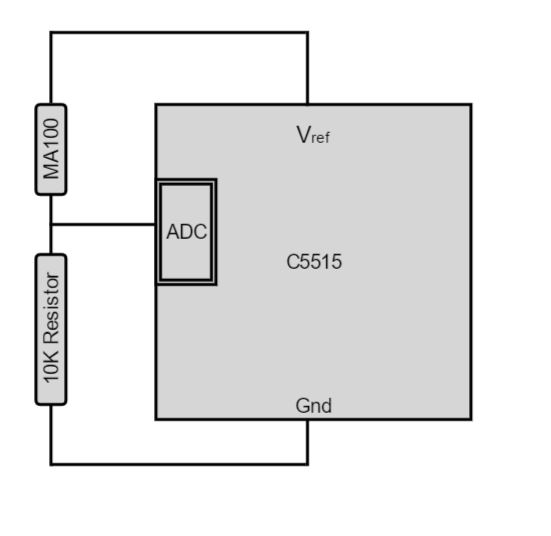
\includegraphics[scale = 0.5 ]{body_temp.JPG}
 	\caption{Simplified version Body Temperature measurement circuitry\label{body_temp}}
 \end{figure}
 
 The C5515 DSP supplies the reference voltage to the thermistor MA100. As body temperature is measured only once in a second, the reference voltage could be supplied only during the measurement and can be turned off the rest of the time to save the power dissipated by the measurement circuit during the unused time.
 
 From \ref{mpu9250_def} it can be noticed that the Accelerometer sensor(MPU9250) takes 30ms to wakeup from sleep and generate a valid accelerometer  value. BlueBox cannot afford to spend this time inside the ISR. So it is a good idea to keep the MPU9250 under low-power accelerometer mode, which consumes 19.8 $\mu$A providing the required response time.
 
 \subsection{Smart Sensing}
 Smart sensing is a method for achieving low power that uses integrated 'smart' digital logic in the sensor. "Smart Sensing" is the added digital capability which can be used to enable the sensor to perform its own internal power management or help reduce the power consumption of the system. This approach has been used in BlueBox through the smart capabilities of accelerometer.
 
The sensor's embedded logic detects events and notifies the DSP over interrupt. Unlike the previous low-power method that has no power consumption at its lowest level, this one has a baseline power consumption, so it can automatically power itself on. With a higher frequency of use, a device with more internal intelligence eventually becomes more efficient. 
 
 An example of such technique in the BlueBox, for reducing power consumption is the use of
 accelerometer’s smart first in, first out (FIFO) buffer. An 8-bit or 12-bit configurable 32-sample 
 FIFO allows buffering of the data so a host system can power on the sensor and read the 
 data at a slower rate. As a result, the DSP can be kept in a lower power state more of 
 the time, achieving lower power consumption for itself and lower duty cycle operation for 
 the DSP whose power consumption can be hundreds or even a thousand times 
 higher than the accelerometer’s power consumption. By reducing the DSP’s power 
 on time by a mere 0.5 \%, the system consumes less power even though the accelerometer 
 consumes more power. The system-level advantages more than compensate for the slightly 
 higher power consumption in the sensor. 
 
 \subsection{Computational offloading}
 In this third approach for low power sensing, the DSP utilizes the local computing capability of the sensor. Termed "local compute capability", this system level methodology can offload the computation from system application DSP . For example, a DSP that uses 100 to 1000 times as much power, a local sensor with the compute capability can perform the required computations and allow the DSP to go into lower power modes delivers a significant power savings at the system level, resulting in savings.  
 
  \begin{figure}[h]
 	\centering
 	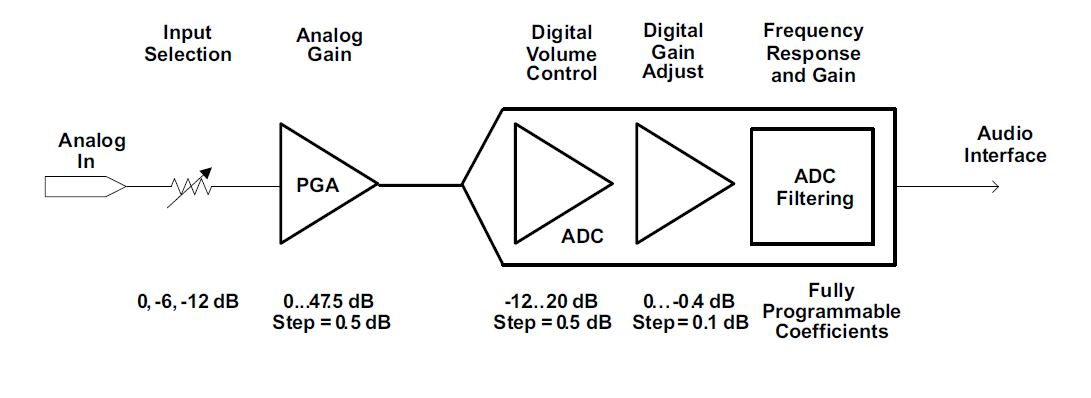
\includegraphics[scale = 0.5 ]{AIC_processingBlock.JPG}
 	\caption{Signal Processing blocks of Audio Codec. Source \cite{audiocodec} \label{AIC_processingBlock}}
 \end{figure}
 
 This design methodology is used in BlueBox to reduce the power consumption of audio data acquisition through the use of local compute capability of the Audio Codec. Audio signal captured through the electret microphones contains some noise with it. And is required to filter the signal to improve the audio quality and attenuate high frequency noises. The process of digital filtering at the DSP could be a good solution as the filter can be designed specific for the application and the signal of interest. But it consumes lots of computational bandwidth and power which is not very desirable for the BlueBox application. So BlueBox uses the signal processing support extended by the audio codec AIC3204 as shown in figure \ref{AIC_processingBlock}. The codec has a fixed number of filters with configurable coefficients. Offloading the digital filtering computation to the codec saves a significant amount of computational bandwidth and power.
 
\section{Power Management of DSP subsystem }

Selecting a processor is one of the most critical decisions when we are designing an embedded 
system. This selection is based on the features required to satisfy the control functionality of the final product and the raw computing power needed to fulfill those system requirements. There are several points to be aware of when selecting a processor. The overall power consumption of a MCU is defined by its power consumption in different modes, typically active and standby (including sleep, idle,standby, etc.),  and taking into account the power consumed to transition from one mode to another. 

Active power consumption by a processor is the power consumed when the processor is running. As almost all controllers are based upon CMOS logic, power is consumed primarily during the switching of transistors. The other major factor which determines the run time of the system is the standby power consumption. Most applications can spend significant amount of time in standby mode. Standby current is the sum of leakage current, current consumed by power management circuits, clocking systems, power regulators, RTC, IOs, interrupt controllers, and so on. It varies from controller to controller, based upon the particular features and peripherals supported in standby mode.  
The power consumed in standby mode is significantly very less than in active mode. So the basic idea is to put the processor into standby mode when ever it is possible and try to keep the processor idle as long as possible to reduce the power consumed by the processor. The following section discusses the techniques used in the BlueBox system to reduce the processor power consumption. 
Timing analysis is the first step towards the understanding of the processor functionality in terms of processor utilization \cite{sastra}. The processor utilization 'U' is defined as the total amount of time spent idle by the processor. 
\[ U = 100\% - (\% T_{idle}) \hspace{20mm} (1)\]

Idle time is the time during which processor does not do any useful work. Normally this is an infinite loop that spins the processor waiting for an event. The code composer studio IDE ,which is used for firmware development,  provides the timing analysis of the code execution in DSP. Once the average idle time is known, we can measure the active utilization when the system is under various states of loads using the equation 1. BlueBox employs Intelligent waiting, even reduction and intelligent peripheral shutdown techniques to reduce the power consumption of the DSP. The following sections explains each of the technique in detail. 

\subsection{Intelligent Waiting}
The TMS320C5515 DSP includes various run-time power modes that can be used to scale down power consumption. The most common of important is idle mode of operation, in which the instruction-executing portion of the processor core shuts down while all peripherals and interrupts remain powered and active.Idle mode consumes substantially less power than the 
processor is actively executing instructions. A key aspect of idle mode is that it requires little overhead to enter and exit, usually allowing it to be applied many times every millisecond. Anytime the DSP is spinning in a loop or blocked waiting for an event it should be placed into idle mode to conserve power. Since any interrupt can wake the DSP from idle mode, use of this mode enables the DSP to intelligently wait for events in the system.  
The BlueBox system is dependent on external interrupts generated by the ECG analog frontend and the audio codec through the I2S bus.From figure \ref{main} it can be seen that the main thread of the BlueBox goes to idle mode after writing the pages to SD card , if they are available. When an interrupt occurs, the DSP wakes up and interrupt is serviced. Then the DSP checks if any page is available to write and then goes back into the idle mode to save power. 


\subsection{Event reduction}
Another important technique employed is the event reduction. Intelligent waiting enables the processor to enter its idle mode as often as possible, event reduction attempts to keep the processor in idle mode as long as possible. It is implemented by analyzing the application firmware code and system requirements to determine the effect of alteration of processing the 
interrupts. 
The interrupts associated with the BlueBox are periodic external interrupts that informs the processor to read an collect the data. There are totally 24000 audio interrupts generated every second by the audio codec. If the processor handles all the interrupts, it will not have suffient time to go to idle mode and have to be active all the time. This is where Direct Memory Access(DMA) comes into play to help the processor. Direct memory access (DMA) allows the processor to remain in idle mode for significant periods even while data is being sent to 
or received from peripherals. DMA should be used in peripheral drivers whenever possible. The savings are quite impressive. The DMA employed with the audio codec reduces 24000 interrupts per second to 24 interrupt per second. Figure \ref{event_reduction} explains how the reduction is achieved.
 \begin{figure}[h]
	\centering
	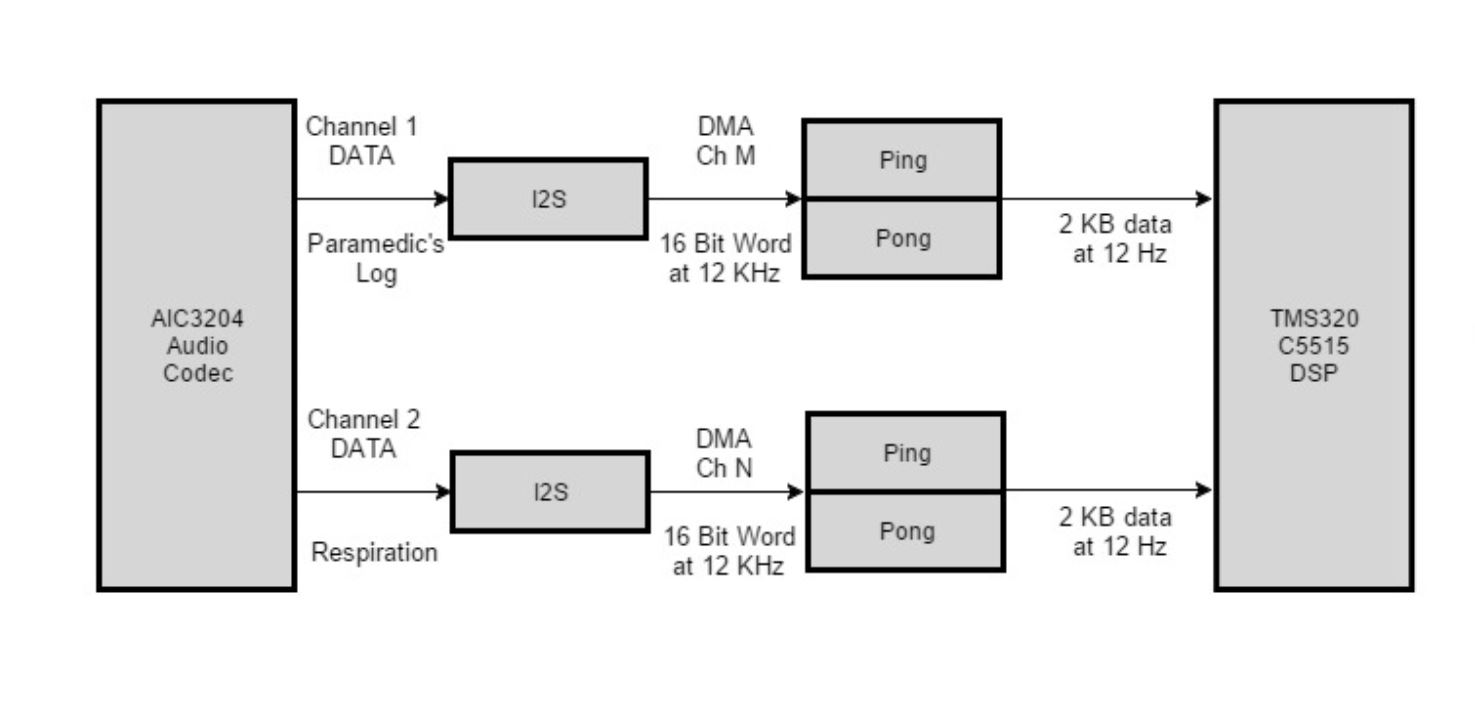
\includegraphics[scale = 0.5 ]{Event_Reduction.JPG}
	\caption{Event Reduction through DMA for Audio acquisition\label{event_reduction}}
\end{figure}


The receiver DMA ping-pong buffer is of 2KB size and it takes 1000 interrupts and move the data into the buffer. When the buffer is full, the DMA interrupts the processor to take further actions. In the mean time the DMA starts servicing the interrupts filling up the pong buffer. Therefore during the situations where the processor is more prone to face the external interrupts, the event reduction approach using the DMA will be the solution.

\subsection{Intelligent peripheral shutdown}
All the above three methods are for the power consumption when the device is running. This method of intelligent shutdown is useful when the peripheral is clock or power gated when it is not in use. The C5515 processor continues to power the general purpose input output pins and peripherals during idle mode. As inputs, these I/O pins can be used as interrupts to wake 
up the device; as outputs, they can be used to configure to external peripherals. Careful configuration of how these pins are configured can have large effect on sleep mode power consumption. 
The DSP has separate power domains which provide power to different portions of the device. The separate power domains allows the firmware to select the optimal voltage to achieve the lowest power consumption at the best possible performance. There are 13 different power domains each of which powers a specific domain. The following table gives the brief gist of the power domains.
\begin{figure}
	\centering
	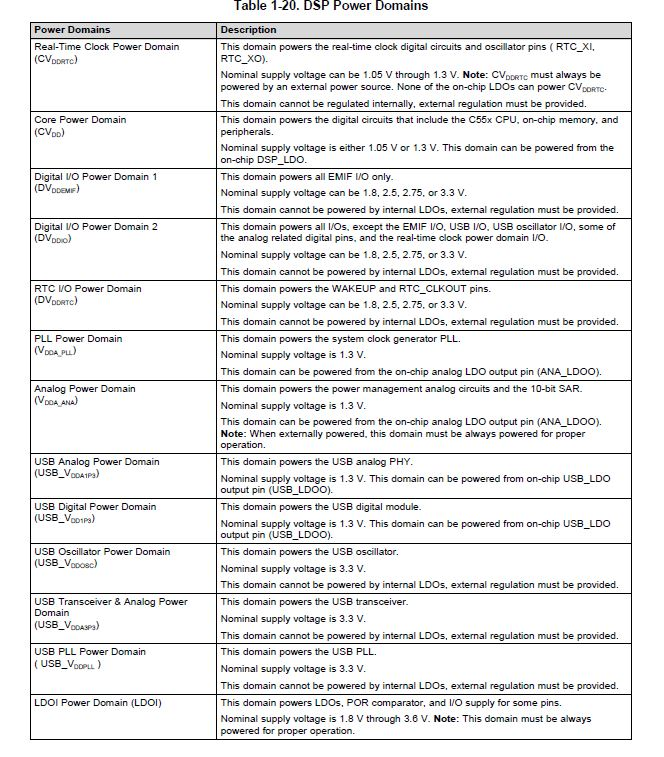
\includegraphics[scale = 1 ]{power_domain.JPG}
	\caption{C5515 DSP power domains. Source\cite{appref}\label{power_domain}}
\end{figure}
Body temperature is measured once in a second. From figure \ref{body_temp} shows the simplified body temperature measurement circuitry. It can be understood that the ADC peripheral of the DSP will be used only once every second. So BlueBox firmware enables the Analog power domain that powers the ADC only during the measurement. The figure \ref{power_domain} shows the active power domains during the different phases of the firmware operation .

\section{Power management of Storage Subsystem}
Storage contributes to a significant fraction of power consumption of embedded system. With respect todata acquisition and logging system the fraction is somewhere between 30 to 50 \% . From the table \ref{table:power_rating} we can notice that power consumption of SDHC card is approximately equal to 50\% of the entire system when a read or write action is performed. It is thus required to manage the storage sub-sytem with atmost care. So the basic idea is to write or read as minimum as possible and only when it is required.
Storage subsystem involves the SDHC card and MMCSD interface from the DSP. As mentioned in section \ref{memory} SDHC card is block addressable. Blocks of size 512 bytes can be written or read from the SD card. So the processor has to buffer blocks of data and write them into the SD card.  

The five different signals have to be stored in the SD card. BlueBox system groups these signals into two category. One just has the audio signal and other has ECG, accelerometer and temperature data. There are buffers associated with each of these categories and the respective data is written into them and eventually flushed to the SD card. The reason for such categorization is because of the amount of data produced by these signals. Audio data is produces at a rate of 48 kilobyte every second, so they need dedicated buffer for themselves to be stored. The other signals are sampled comparitvely very less, so they could be grouped together to share buffers and are written into the SD card. 

The ECG analog front end interrupts the DSP at a frequency of 500Hz. Each sample collected during the interrupt is appended to the buffer. Because accelerometer only needs to be sampled at 12Hz, a counter within the interrupt ensures that accelerometer is sampled only once every 40 interrupts. Similarly the temperature is to be sampled at 2 Hz, a counter within the interrupt service routine is used to make sure samples are taken every 250 interrupts. Each time the signals are sampled , values from each of the sensors are stored in the respective position in the buffer. 
\subsection{Saving data to micro SD card}

Because the BlueBox must be able to continuously and without interruption, the timer interrupt services must continue to operate even when data is being written to SD card. So DMA's are used to write the data into the SD card as it can do the task without the interference of the DSP.When possible, sampled data is saved directly to a primary data buffer. When the primary data buffer is full DMA is instructed to initiate the transfer of the data from primary buffer into the SD card persistent storage. In the meantime data collected is stored in the secondary buffer and the cycle goes on. 

There are lot of different ways of writing and organizing the data in the SD card. One way is to use existing filesystem that is recognizable by the general operating system, other way is to write the raw data and to design a own file system. There are pro's and con's associated with designing a new file system. Using a existing standard filesystem like FAT 16, FAT 32, NTFS etc are really simple to implement as standard libraries are present but they were all designed for user comfortability and are designed for higher end computational devices. There is a huge overhead associated with storing and reading of data . For example inorder to write a block of data into a file, it takes multiple reads to figure out to which block address it should go and write into that address. This process keeps the SD card busy for longer duration, which is very undesirable for our application. It is required to come up with a simple custom filesystem that could suffice the necessity of application. The problems of custom file system is incompatibility with standard operating system. To read data from the SD card , it is required to develop a file system driver which is capable of reading this SD card and also it requires some time to implement and test the custom file system. The important thing here to notice is that the custom filesystem could potentially save time and power it consumes to write data to the SD card. The following section gives a brief description of the filesystem used in BlueBox. 

\subsection{File System}\label{filesystem}
A Secure Digital High Capacity(SD) card basically has a SD controller module and a memory core. Memory core is where the data is stored in. The memory core of a SDHC card is divided into blocks of 512 bytes and they are block addressable.  BlueBox caches the data in a local buffer, which  are, in general multiples of block size of the SD card. For convenience of understanding, the buffer that caches the data is referred as pages. The custom filesystem developed for bluebox has three categories of pages. They are audio page(same page layout used for both the channels of audio), vitals page(includes ECG, temperature and accelerometer data) and index page. The page size used for audio is 2Kb and for ECG its 512 bytes.
 Figure \ref{audio_page} shows the layout of audio page. Size of an audio page is 2 kilobytes, which is four blocks.It just contains the actual data and does not encode any meta-data with it. The pointers to the audio pages are present in the Index page. Each audio page accounts for four blocks, so when ever an audio page is written to the SD card, the corresponding four block address are stored in the index page. 
\begin{figure}[h]
	\centering
	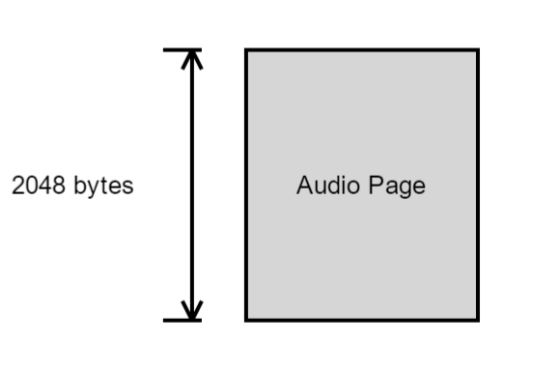
\includegraphics[scale = 0.5 ]{audio_page.JPG}
	\caption{Audio Page\label{audio_page}}
\end{figure}


 Figure \ref{vital_page} depicts the Vitals page. Its 512 bytes in size and contains actual data along with meta data. The first two bytes of the vitals page is an identifier , which uniquely identifies it. It includes ECG, accelerometer , temperature and time data. 

\begin{figure}[h]
	\centering
	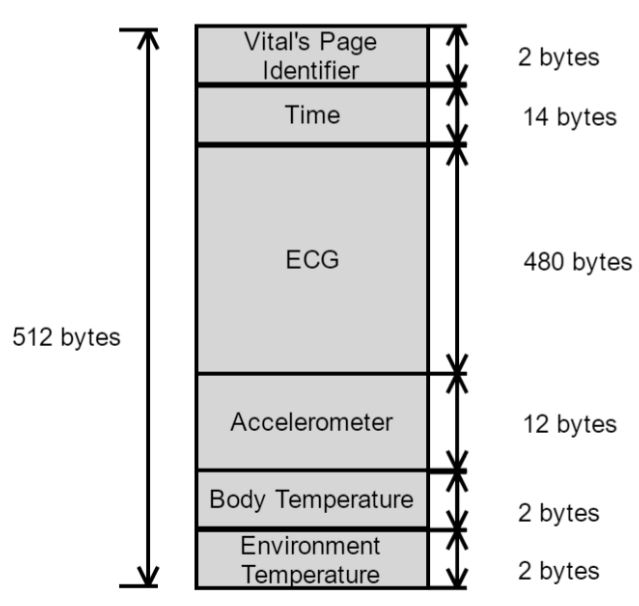
\includegraphics[scale = 0.5 ]{vital_page.JPG}
	\caption{Vitals Page\label{vital_page}}
\end{figure}

The index page comprises of a 2 byte page identifier, 2 byte Audio channel identifier and 127 32bit block address as shown in figure \ref{index_page}.There is a separate index pages for left and right channel audio.The block addresses in the index pages are the pointers to next pieces of the audio data.The audio data is reconstructed into a file using these index pages.

Index page description: 
\begin{figure}[h]
	\centering
	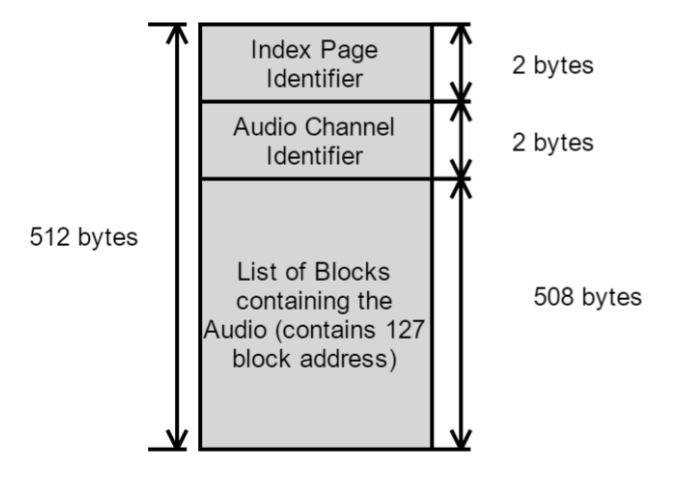
\includegraphics[scale = 0.5 ]{index_page.JPG}
	\caption{Index Page\label{index_page}}
\end{figure}

The firmware filesystem driver keeps track of the next available free block and decides to which block does the page of data go into. All the pages are written to the SD card sequentially. After the page has been successfully written by the DMA, the block address pointer is updated to point to the next free block.  24 pages of audio sample is written per second and 4 pages of ECG and other aggregated data is written per second.  
Also the filesystem keeps track of which block of the storage has which type of page through page identifiers and the pointers in the index page. The index page is also stored in an in memory buffer and when it fills up it is written into the SD card. So that while reading back the data from the SD card we could organize the blocks and reconstruct the data stream.  

This simple custom filesystem  helped in reducing the overhead of writing data to SD card , which in general is very high with a standard file system that adds up bunch of meta data. The following graph \ref{fig:fs_time} shows the time taken to write the data to sd card and compares the two file system. The x axis marks the amount of data( includes only the meaningful sensor data)  and the y axis marks time in millisecond.

\begin{tikzpicture}
\begin{axis}[
title={SDHC card data write time},
xmode=log,
ymode=log,
height =100mm,
width = 100mm,
xlabel={ Data size [KB]},
ylabel={Time [ms] },
xmin=0, xmax=1000,
ymin=0, ymax=20000,
xtick={0.1,1,10,100,1000},
ytick={0.1,1,10,1000,10000,100000},
legend pos=north west,
ymajorgrids=true,
grid style=dashed,
]

\addplot[
color=blue,
mark=square,
]
coordinates {
	(0.5,0.21)(1,0.52)(10,3.02)(100,30.28)(1000,333.09)

};
\addlegendentry{Custom FileSystem}

\addplot[
color=black,
mark=*,
]
coordinates {
	(0.5,20.644)(1,77.15)(10,133.70)(100,1517.986)(1000,16552.70)
	
};
\addlegendentry{FAT FileSystem}

\end{axis}
\end{tikzpicture}\label{fig:fs_time}
From the figure \ref{fig:fs_time} it is evident that for the same amount of actual data the custom filesystem takes, on an average, 50x less time to write than the FAT filesystem. The custom filesystem essentially spends less energy and consumes less power to save the data by reducing the active utilization time by 50x. 


From the experiment with SDHC card,running at 20MHz clock at 3.3 V,  the write/read operation consumes 35mA (considering only DSP and SD card active) and in standby it consumes 22mA. BlueBox system requries to write 50 KB of data every second. With FAT file system, the system consumes average current of 30.5mA when writing 50KB of data in one second whereas the custom file system's average current consumption is 17.27 mA. Thus The designed file system reduces the system power consumption by 50\% within the application semantics of BlueBox. 
\chapter{Experiments and Clinical Test}
This Chapter explains the setup for testing the basic device functionalities and its performance. The Chapter also discusses the clinical test conducted at LA BioMed at Torrance using Mannequin-based Patient Simulation. The study protocol, analysis and preliminary results will be discussed.

\section{Motivation}
The motivation for the study can be broken down into the following:
\begin{itemize}
	\item To perform preliminary testing of device functionalities and to test if the system runtime requirement is fulfilled
	
	\item To perform a clinical test to evaluate the signal quality and to test the usability
	
	\item To obtain suite of signals in a data set for future algorithm optimization
	 
\end{itemize}

\section{Preliminary Experiments and 
	System Characterization}\label{utilization_result}
The basic device functionality of the device is tested by simulating the required signals locally in our lab \ref{fig:sim_test}. The ECG signal is simulated using Precise Life SKX 2000 ECG simulator. The ECG is interfaced in 4 lead configuration using right arm(RA), left arm(LA), left leg(LL) and right leg(RL) drive leads. The body temperature is simulated using sodium acetate based reusable head pods. The acceleration of chest, paramedic log and breathing sound are manually simulated.
\begin{figure}[h]
	\centering
	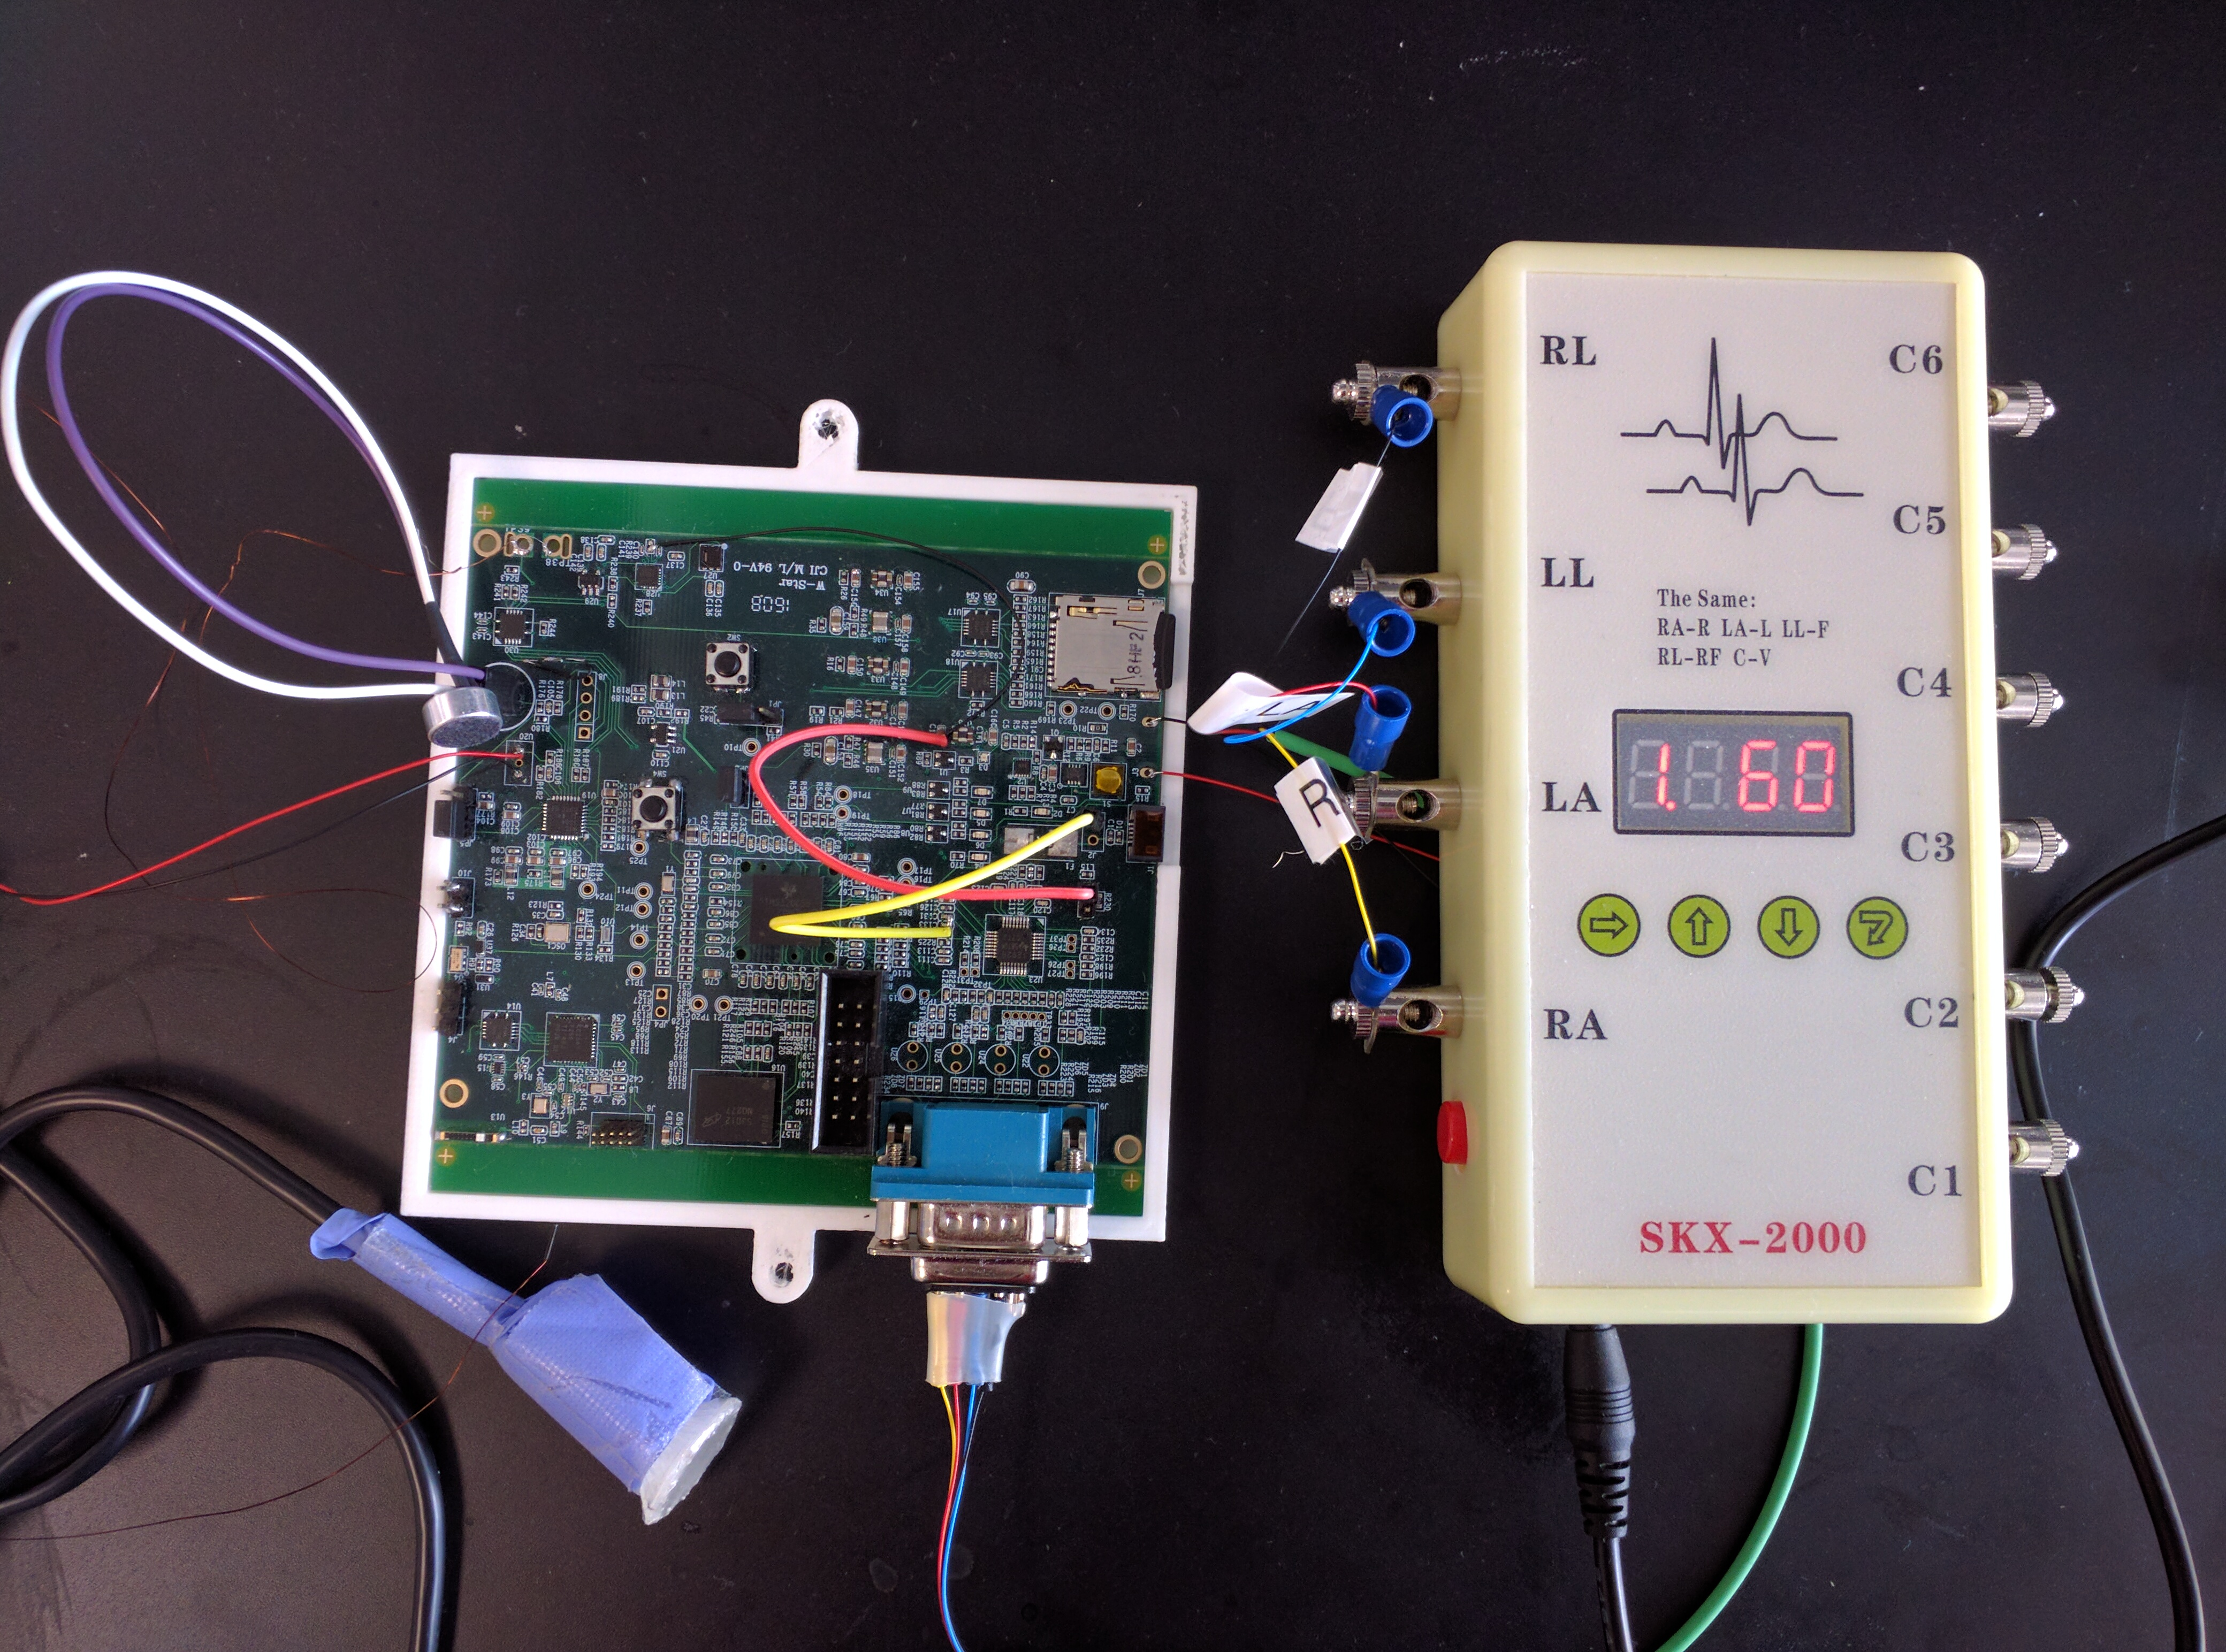
\includegraphics[scale = 0.08 ]{sim_test.JPG}
	\caption{Prototype Test Environment\label{fig:sim_test}}
\end{figure}

The system is tested with the firmware that incorporated the techniques mentioned in the previous chapter. In order to determine the power dissipation, the relative contribution of the different parts of the system needs to be considered. First, the idle mode current of the system was measured to be 22 mA. The environment temperature sensor, ECG front end chip and the accelerometer are powered directly from the battery. They are not controlled by the DSP, so the state of the DSP does not affect their power consumption. These components always contribute towards the current drawn by the system irrespective of the state of DSP. The average current drawn by the system under different modes of operation are shown in table\ref{table:current_drawn}. The average current drawn by the system with all the sensors and DSP (running at 100MHz) being active was measured to be 38.64 mA. The average current drawn when writing to the SD card while all the components of the system are active was measured to be 48 mA. The current drawn by the system was measured using INA231 evaluation module \cite{INA231}, which samples the current drawn by the system every 140 $\mu$S and logs the data.
\begin{table}[h]
	\centering
	\begin{tabular}{|l|l|}
		\hline
		Operation & Current\\
		\hline
		Idle & 22 mA\\
		Data Acquisition & 38.64 mA\\
		Micro SD write & 48 mA \\
		\hline
	\end{tabular}
	\caption{Current drawn for different operation mode.}
	\label{table:current_drawn}
\end{table}

We also measured the DSP utilization to have more insight into how long the system is in different operation mode mentioned above. We used the Code Composer studio's sophisticated profile clock to count the utilization of DSP \cite{clock_profile}. As mentioned in section \ref{firmware_arch} there are three main routines that run: main, DMA ISR and ECG ISR.
The worst case execution time of DMA ISR (WCET\textsubscript{DMA}) routine is 3000 cycles to service the interrupt and it is executed for 24 times in a second. The DMA ISR utilization (U\textsubscript{DMA}) can be calculated as follows:

\vspace*{-2mm}

\[U_{DMA} = \frac{WCET_{DMA} * Number of Interrupts/Second}{
	F_{DSP}
} * 100 \%\]


\vspace*{-2mm}
 \[U_{DMA} = \frac{3000 * 24}{
	100,000,000
} * 100 \% = 0.72\% \]


Where F\textsubscript{DSP} is the frequency at which the DSP is running, which is 100 MHz in our case. Similarly the main routine and the ECG ISR is profiled. The summary of the worst case utilization of these routines are presented in table \ref{table:WCET}. The total utilization of the DSP in active mode is roughly 20.92\%.
\begin{table}[h]
	\centering
	\begin{tabular}{|l|l|}
		\hline
		Routinue & Utilization\\
		\hline
		Main & 18\%\\
		DMA ISR & 0.72\%\\
		ECG ISR & 2.204\% \\
		\hline
	\end{tabular}
	\caption{Current drawn for different operation mode.}
	\label{table:WCET}
\end{table}
 
 The Storage utilization with the custom filesystem is computed to be 1.5\%. The worst case contribution of storage towards the average current drawn by the system is 
 \[ 48 mA* \frac{1.5}{100} = 0.72 mA \]
 
 The average current drawn by the system considering during the idle and active mode:
 
 \[ 38.64 mA* \frac{20.924}{100} + 22 mA * \frac{79.076}{100}  = 25.481 mA\] 
 
The average current drawn by the system sums up to approximately 26.201 mA. With this rate the system should be able to run for 9 - 10 hours before recharging the battery. The acquired data was verfied by primarily reconstructing the signal and confirm if the amount of samples of each signal is equivalent to the test duration. This ensures the correctness of the process of data recording. The validity of the data was verified manually from playing back the signals and validating if the reflected the conditions during the test.
\section{Clinical Test, Setup and Protocol}

\subsection{Mannequin-based Patient Simulation}
BlueBox initial clinical test is done with a Mannequin-based patient simulation environment.
Taking the underlying concepts described for the desktop simulation one step further is the recreation of the real physical patient in a realistic physical clinical environment \cite{man}. Thus, computerized mannequin stands in for the patient, and a variety of equipment can be used (either real clinical equipment or computer-driven replicas) to monitor and treat the patient.
Among the functions that these mannequin-based simulators can replicate are:
\begin{itemize}
	\item Spontaneous breathing (and the ability to breathe for the patient with a bag or ventilator)
	\item Pulses, heart sounds, breath sounds, pupil size, pupil response to light
	
	\item Real-time display of electronically monitored information (e.g. ECG, oxygen saturation, etc.)	
\end{itemize}

Not only are these created in their “normal” manifestation, but all the elements of a large variety of abnormal conditions can be created such as (the list is almost endless) heart attack, severe allergic reaction, breathing difficulties, sepsis (“blood poisoning”), severe abnormalities of sugar metabolism etc.

\subsection{Test Protocol}
The test was done with the BlueBox device placed on the Mannequin's chest. The Mannequin wore the four electrode model in a lead II configuration. The body temperature sensor is worn near the mannequin's neck. The contact mirophone to record the respiration sound is placed on the mannequin's abdomen. The environment microphone to record paramedic's comments is on the top of the device. As the accelerometer is on board, it can measure the chest rise of the mannequin. The on-board temperature sensor can measure environment temperature. The preliminary tests were conducted for different time duration ranging from 15 minutes to 2 hours. The tests were conducted under normal conditions and variety of abnormal conditions like heart attack, severe allergic reaction, breathing difficulties etc. The device is switched on using a button during the beginning of th experiment and after the test duration is completed, the data is imported into the computer to verify if the signal reflected the test conditions. The lab researchers and doctors on the IRB are required to be present for the duration of the test. 

\section{Analysis and Result}
The important objective of the test is to evaluate the signal quality and performance of the BlueBox device. This is achieved by comparing the acquired signal with the originally simulated signals. The computerized mannequin has a record of all physically simulated signals (including ECG, breathing pattern and body temperature). All the vitals are compared with the original signal for evaluation. The two ECG signals are aligned in time to make a simple analysis. By analyzing these two signals physicians concluded that the acquired signal is reliable. Body temperature and chest movements were also analyzed with the same manner and are reliable. The following figures shows the samples of results of signals measured during the Clinical tests.


\begin{tikzpicture}
\begin{axis}[
title={ECG Signal},
height =60mm,
width = 160mm,
xlabel={ Time [Seconds]},
ylabel={Voltage [mV]},
xmin=0, xmax=10,
ymin=4, ymax=10.5,
xtick={0,1,2,3,4,5,6,7,8,9,10},
ytick={4,5,6,7,8,9,10},
legend pos=north west,
ymajorgrids=true,
grid style=dashed,
]

\addplot[
color=blue,
mark=.,
]
coordinates {
	(0.000000,6.729260)
	(0.002000,6.722963)
	(0.004000,6.717216)
	(0.006000,6.712029)
	(0.008000,6.707477)
	(0.010000,6.703690)
	(0.012000,6.700802)
	(0.014000,6.698903)
	(0.016000,6.698000)
	(0.018000,6.698016)
	(0.020000,6.698823)
	(0.022000,6.700307)
	(0.024000,6.702413)
	(0.026000,6.705151)
	(0.028000,6.708559)
	(0.030000,6.712656)
	(0.032000,6.717393)
	(0.034000,6.722645)
	(0.036000,6.728231)
	(0.038000,6.733976)
	(0.040000,6.739759)
	(0.042000,6.745540)
	(0.044000,6.751335)
	(0.046000,6.757169)
	(0.048000,6.763028)
	(0.050000,6.768831)
	(0.052000,6.774445)
	(0.054000,6.779733)
	(0.056000,6.784616)
	(0.058000,6.789103)
	(0.060000,6.793280)
	(0.062000,6.797256)
	(0.064000,6.801113)
	(0.066000,6.804863)
	(0.068000,6.808447)
	(0.070000,6.811769)
	(0.072000,6.814760)
	(0.074000,6.817417)
	(0.076000,6.819807)
	(0.078000,6.822028)
	(0.080000,6.824156)
	(0.082000,6.826202)
	(0.084000,6.828098)
	(0.086000,6.829724)
	(0.088000,6.830964)
	(0.090000,6.831764)
	(0.092000,6.832146)
	(0.094000,6.832187)
	(0.096000,6.831963)
	(0.098000,6.831507)
	(0.100000,6.830783)
	(0.102000,6.829698)
	(0.104000,6.828158)
	(0.106000,6.826123)
	(0.108000,6.823643)
	(0.110000,6.820841)
	(0.112000,6.817860)
	(0.114000,6.814809)
	(0.116000,6.811729)
	(0.118000,6.808578)
	(0.120000,6.805278)
	(0.122000,6.801771)
	(0.124000,6.798066)
	(0.126000,6.794236)
	(0.128000,6.790388)
	(0.130000,6.786601)
	(0.132000,6.782893)
	(0.134000,6.779206)
	(0.136000,6.775433)
	(0.138000,6.771479)
	(0.140000,6.767315)
	(0.142000,6.762994)
	(0.144000,6.758620)
	(0.146000,6.754298)
	(0.148000,6.750086)
	(0.150000,6.745974)
	(0.152000,6.741894)
	(0.154000,6.737772)
	(0.156000,6.733588)
	(0.158000,6.729402)
	(0.160000,6.725337)
	(0.162000,6.721531)
	(0.164000,6.718085)
	(0.166000,6.715026)
	(0.168000,6.712312)
	(0.170000,6.709862)
	(0.172000,6.707627)
	(0.174000,6.705620)
	(0.176000,6.703925)
	(0.178000,6.702653)
	(0.180000,6.701894)
	(0.182000,6.701675)
	(0.184000,6.701948)
	(0.186000,6.702617)
	(0.188000,6.703600)
	(0.190000,6.704884)
	(0.192000,6.706533)
	(0.194000,6.708658)
	(0.196000,6.711363)
	(0.198000,6.714693)
	(0.200000,6.718611)
	(0.202000,6.723013)
	(0.204000,6.727780)
	(0.206000,6.732836)
	(0.208000,6.738178)
	(0.210000,6.743855)
	(0.212000,6.749923)
	(0.214000,6.756389)
	(0.216000,6.763184)
	(0.218000,6.770164)
	(0.220000,6.777151)
	(0.222000,6.784002)
	(0.224000,6.790646)
	(0.226000,6.797086)
	(0.228000,6.803357)
	(0.230000,6.809471)
	(0.232000,6.815384)
	(0.234000,6.820979)
	(0.236000,6.826104)
	(0.238000,6.830621)
	(0.240000,6.834463)
	(0.242000,6.837644)
	(0.244000,6.840225)
	(0.246000,6.842265)
	(0.248000,6.843781)
	(0.250000,6.844721)
	(0.252000,6.844986)
	(0.254000,6.844483)
	(0.256000,6.843186)
	(0.258000,6.841165)
	(0.260000,6.838566)
	(0.262000,6.835554)
	(0.264000,6.832261)
	(0.266000,6.828752)
	(0.268000,6.825025)
	(0.270000,6.821051)
	(0.272000,6.816836)
	(0.274000,6.812459)
	(0.276000,6.808062)
	(0.278000,6.803808)
	(0.280000,6.799825)
	(0.282000,6.796172)
	(0.284000,6.792823)
	(0.286000,6.789705)
	(0.288000,6.786753)
	(0.290000,6.783967)
	(0.292000,6.781414)
	(0.294000,6.779201)
	(0.296000,6.777419)
	(0.298000,6.776096)
	(0.300000,6.775179)
	(0.302000,6.774548)
	(0.304000,6.774075)
	(0.306000,6.773685)
	(0.308000,6.773385)
	(0.310000,6.773245)
	(0.312000,6.773348)
	(0.314000,6.773749)
	(0.316000,6.774442)
	(0.318000,6.775370)
	(0.320000,6.776475)
	(0.322000,6.777763)
	(0.324000,6.779338)
	(0.326000,6.781394)
	(0.328000,6.784155)
	(0.330000,6.787822)
	(0.332000,6.792522)
	(0.334000,6.798298)
	(0.336000,6.805143)
	(0.338000,6.813053)
	(0.340000,6.822084)
	(0.342000,6.832346)
	(0.344000,6.843976)
	(0.346000,6.857073)
	(0.348000,6.871656)
	(0.350000,6.887646)
	(0.352000,6.904888)
	(0.354000,6.923212)
	(0.356000,6.942495)
	(0.358000,6.962690)
	(0.360000,6.983800)
	(0.362000,7.005826)
	(0.364000,7.028716)
	(0.366000,7.052341)
	(0.368000,7.076495)
	(0.370000,7.100954)
	(0.372000,7.125534)
	(0.374000,7.150128)
	(0.376000,7.174700)
	(0.378000,7.199236)
	(0.380000,7.223688)
	(0.382000,7.247939)
	(0.384000,7.271796)
	(0.386000,7.295031)
	(0.388000,7.317440)
	(0.390000,7.338895)
	(0.392000,7.359350)
	(0.394000,7.378798)
	(0.396000,7.397218)
	(0.398000,7.414530)
	(0.400000,7.430575)
	(0.402000,7.445136)
	(0.404000,7.457993)
	(0.406000,7.468988)
	(0.408000,7.478043)
	(0.410000,7.485138)
	(0.412000,7.490270)
	(0.414000,7.493397)
	(0.416000,7.494418)
	(0.418000,7.493179)
	(0.420000,7.489525)
	(0.422000,7.483358)
	(0.424000,7.474683)
	(0.426000,7.463591)
	(0.428000,7.450216)
	(0.430000,7.434686)
	(0.432000,7.417087)
	(0.434000,7.397450)
	(0.436000,7.375794)
	(0.438000,7.352180)
	(0.440000,7.326758)
	(0.442000,7.299768)
	(0.444000,7.271503)
	(0.446000,7.242253)
	(0.448000,7.212256)
	(0.450000,7.181678)
	(0.452000,7.150635)
	(0.454000,7.119246)
	(0.456000,7.087688)
	(0.458000,7.056216)
	(0.460000,7.025128)
	(0.462000,6.994719)
	(0.464000,6.965225)
	(0.466000,6.936809)
	(0.468000,6.909566)
	(0.470000,6.883596)
	(0.472000,6.859072)
	(0.474000,6.836285)
	(0.476000,6.815633)
	(0.478000,6.797564)
	(0.480000,6.782518)
	(0.482000,6.770907)
	(0.484000,6.763134)
	(0.486000,6.759658)
	(0.488000,6.761077)
	(0.490000,6.768171)
	(0.492000,6.781886)
	(0.494000,6.803238)
	(0.496000,6.833199)
	(0.498000,6.872620)
	(0.500000,6.922189)
	(0.502000,6.982437)
	(0.504000,7.053779)
	(0.506000,7.136532)
	(0.508000,7.230907)
	(0.510000,7.336948)
	(0.512000,7.454457)
	(0.514000,7.582925)
	(0.516000,7.721491)
	(0.518000,7.868942)
	(0.520000,8.023761)
	(0.522000,8.184209)
	(0.524000,8.348383)
	(0.526000,8.514252)
	(0.528000,8.679675)
	(0.530000,8.842405)
	(0.532000,9.000112)
	(0.534000,9.150415)
	(0.536000,9.290966)
	(0.538000,9.419552)
	(0.540000,9.534176)
	(0.542000,9.633104)
	(0.544000,9.714856)
	(0.546000,9.778185)
	(0.548000,9.822056)
	(0.550000,9.845638)
	(0.552000,9.848341)
	(0.554000,9.829871)
	(0.556000,9.790282)
	(0.558000,9.729981)
	(0.560000,9.649684)
	(0.562000,9.550350)
	(0.564000,9.433107)
	(0.566000,9.299209)
	(0.568000,9.150017)
	(0.570000,8.987027)
	(0.572000,8.811901)
	(0.574000,8.626473)
	(0.576000,8.432702)
	(0.578000,8.232606)
	(0.580000,8.028179)
	(0.582000,7.821337)
	(0.584000,7.613892)
	(0.586000,7.407577)
	(0.588000,7.204083)
	(0.590000,7.005096)
	(0.592000,6.812277)
	(0.594000,6.627212)
	(0.596000,6.451343)
	(0.598000,6.285918)
	(0.600000,6.131970)
	(0.602000,5.990338)
	(0.604000,5.861727)
	(0.606000,5.746755)
	(0.608000,5.645972)
	(0.610000,5.559826)
	(0.612000,5.488611)
	(0.614000,5.432424)
	(0.616000,5.391147)
	(0.618000,5.364469)
	(0.620000,5.351949)
	(0.622000,5.353085)
	(0.624000,5.367353)
	(0.626000,5.394195)
	(0.628000,5.432983)
	(0.630000,5.482971)
	(0.632000,5.543281)
	(0.634000,5.612911)
	(0.636000,5.690791)
	(0.638000,5.775861)
	(0.640000,5.867118)
	(0.642000,5.963626)
	(0.644000,6.064477)
	(0.646000,6.168748)
	(0.648000,6.275467)
	(0.650000,6.383612)
	(0.652000,6.492151)
	(0.654000,6.600110)
	(0.656000,6.706633)
	(0.658000,6.811005)
	(0.660000,6.912618)
	(0.662000,7.010920)
	(0.664000,7.105376)
	(0.666000,7.195443)
	(0.668000,7.280596)
	(0.670000,7.360384)
	(0.672000,7.434488)
	(0.674000,7.502748)
	(0.676000,7.565138)
	(0.678000,7.621707)
	(0.680000,7.672523)
	(0.682000,7.717635)
	(0.684000,7.757074)
	(0.686000,7.790895)
	(0.688000,7.819239)
	(0.690000,7.842368)
	(0.692000,7.860652)
	(0.694000,7.874515)
	(0.696000,7.884375)
	(0.698000,7.890601)
	(0.700000,7.893504)
	(0.702000,7.893371)
	(0.704000,7.890524)
	(0.706000,7.885377)
	(0.708000,7.878433)
	(0.710000,7.870243)
	(0.712000,7.861338)
	(0.714000,7.852171)
	(0.716000,7.843100)
	(0.718000,7.834400)
	(0.720000,7.826320)
	(0.722000,7.819143)
	(0.724000,7.813206)
	(0.726000,7.808877)
	(0.728000,7.806491)
	(0.730000,7.806302)
	(0.732000,7.808445)
	(0.734000,7.812949)
	(0.736000,7.819782)
	(0.738000,7.828916)
	(0.740000,7.840370)
	(0.742000,7.854196)
	(0.744000,7.870436)
	(0.746000,7.889059)
	(0.748000,7.909927)
	(0.750000,7.932791)
	(0.752000,7.957327)
	(0.754000,7.983210)
	(0.756000,8.010167)
	(0.758000,8.037988)
	(0.760000,8.066496)
	(0.762000,8.095485)
	(0.764000,8.124682)
	(0.766000,8.153725)
	(0.768000,8.182191)
	(0.770000,8.209655)
	(0.772000,8.235751)
	(0.774000,8.260204)
	(0.776000,8.282807)
	(0.778000,8.303370)
	(0.780000,8.321672)
	(0.782000,8.337433)
	(0.784000,8.350316)
	(0.786000,8.359975)
	(0.788000,8.366123)
	(0.790000,8.368567)
	(0.792000,8.367205)
	(0.794000,8.361984)
	(0.796000,8.352856)
	(0.798000,8.339737)
	(0.800000,8.322508)
	(0.802000,8.301048)
	(0.804000,8.275295)
	(0.806000,8.245302)
	(0.808000,8.211237)
	(0.810000,8.173349)
	(0.812000,8.131912)
	(0.814000,8.087175)
	(0.816000,8.039341)
	(0.818000,7.988584)
	(0.820000,7.935097)
	(0.822000,7.879151)
	(0.824000,7.821111)
	(0.826000,7.761406)
	(0.828000,7.700481)
	(0.830000,7.638740)
	(0.832000,7.576516)
	(0.834000,7.514071)
	(0.836000,7.451639)
	(0.838000,7.389486)
	(0.840000,7.327946)
	(0.842000,7.267403)
	(0.844000,7.208250)
	(0.846000,7.150833)
	(0.848000,7.095413)
	(0.850000,7.042157)
	(0.852000,6.991173)
	(0.854000,6.942571)
	(0.856000,6.896506)
	(0.858000,6.853186)
	(0.860000,6.812835)
	(0.862000,6.775640)
	(0.864000,6.741704)
	(0.866000,6.711035)
	(0.868000,6.683561)
	(0.870000,6.659196)
	(0.872000,6.637891)
	(0.874000,6.619657)
	(0.876000,6.604542)
	(0.878000,6.592576)
	(0.880000,6.583721)
	(0.882000,6.577845)
	(0.884000,6.574726)
	(0.886000,6.574105)
	(0.888000,6.575743)
	(0.890000,6.579465)
	(0.892000,6.585146)
	(0.894000,6.592674)
	(0.896000,6.601900)
	(0.898000,6.612606)
	(0.900000,6.624505)
	(0.902000,6.637280)
	(0.904000,6.650648)
	(0.906000,6.664403)
	(0.908000,6.678427)
	(0.910000,6.692647)
	(0.912000,6.706984)
	(0.914000,6.721313)
	(0.916000,6.735446)
	(0.918000,6.749152)
	(0.920000,6.762221)
	(0.922000,6.774514)
	(0.924000,6.785985)
	(0.926000,6.796657)
	(0.928000,6.806565)
	(0.930000,6.815711)
	(0.932000,6.824034)
	(0.934000,6.831419)
	(0.936000,6.837745)
	(0.938000,6.842940)
	(0.940000,6.847019)
	(0.942000,6.850064)
	(0.944000,6.852190)
	(0.946000,6.853486)
	(0.948000,6.853987)
	(0.950000,6.853665)
	(0.952000,6.852472)
	(0.954000,6.850398)
	(0.956000,6.847513)
	(0.958000,6.843969)
	(0.960000,6.839960)
	(0.962000,6.835664)
	(0.964000,6.831199)
	(0.966000,6.826609)
	(0.968000,6.821883)
	(0.970000,6.817018)
	(0.972000,6.812066)
	(0.974000,6.807154)
	(0.976000,6.802451)
	(0.978000,6.798116)
	(0.980000,6.794249)
	(0.982000,6.790863)
	(0.984000,6.787898)
	(0.986000,6.785267)
	(0.988000,6.782918)
	(0.990000,6.780872)
	(0.992000,6.779202)
	(0.994000,6.777996)
	(0.996000,6.777298)
	(0.998000,6.777081)
	(1.000000,6.777243)
	(1.002000,6.777648)
	(1.004000,6.778186)
	(1.006000,6.778815)
	(1.008000,6.779567)
	(1.010000,6.780507)
	(1.012000,6.781684)
	(1.014000,6.783092)
	(1.016000,6.784651)
	(1.018000,6.786242)
	(1.020000,6.787760)
	(1.022000,6.789177)
	(1.024000,6.790551)
	(1.026000,6.791997)
	(1.028000,6.793635)
	(1.030000,6.795535)
	(1.032000,6.797693)
	(1.034000,6.800039)
	(1.036000,6.802492)
	(1.038000,6.805012)
	(1.040000,6.807636)
	(1.042000,6.810454)
	(1.044000,6.813561)
	(1.046000,6.817009)
	(1.048000,6.820769)
	(1.050000,6.824729)
	(1.052000,6.828738)
	(1.054000,6.832668)
	(1.056000,6.836457)
	(1.058000,6.840114)
	(1.060000,6.843676)
	(1.062000,6.847160)
	(1.064000,6.850522)
	(1.066000,6.853643)
	(1.068000,6.856365)
	(1.070000,6.858541)
	(1.072000,6.860099)
	(1.074000,6.861050)
	(1.076000,6.861464)
	(1.078000,6.861415)
	(1.080000,6.860941)
	(1.082000,6.860011)
	(1.084000,6.858544)
	(1.086000,6.856458)
	(1.088000,6.853735)
	(1.090000,6.850448)
	(1.092000,6.846741)
	(1.094000,6.842780)
	(1.096000,6.838697)
	(1.098000,6.834555)
	(1.100000,6.830346)
	(1.102000,6.826026)
	(1.104000,6.821583)
	(1.106000,6.817068)
	(1.108000,6.812601)
	(1.110000,6.808321)
	(1.112000,6.804339)
	(1.114000,6.800697)
	(1.116000,6.797354)
	(1.118000,6.794219)
	(1.120000,6.791211)
	(1.122000,6.788310)
	(1.124000,6.785566)
	(1.126000,6.783075)
	(1.128000,6.780920)
	(1.130000,6.779128)
	(1.132000,6.777652)
	(1.134000,6.776382)
	(1.136000,6.775201)
	(1.138000,6.774042)
	(1.140000,6.772913)
	(1.142000,6.771878)
	(1.144000,6.771010)
	(1.146000,6.770344)
	(1.148000,6.769844)
	(1.150000,6.769408)
	(1.152000,6.768912)
	(1.154000,6.768277)
	(1.156000,6.767510)
	(1.158000,6.766698)
	(1.160000,6.765968)
	(1.162000,6.765426)
	(1.164000,6.765118)
	(1.166000,6.765014)
	(1.168000,6.765041)
	(1.170000,6.765141)
	(1.172000,6.765318)
	(1.174000,6.765648)
	(1.176000,6.766246)
	(1.178000,6.767212)
	(1.180000,6.768585)
	(1.182000,6.770319)
	(1.184000,6.772307)
	(1.186000,6.774429)
	(1.188000,6.776616)
	(1.190000,6.778874)
	(1.192000,6.781268)
	(1.194000,6.783868)
	(1.196000,6.786702)
	(1.198000,6.789725)
	(1.200000,6.792825)
	(1.202000,6.795867)
	(1.204000,6.798752)
	(1.206000,6.801460)
	(1.208000,6.804035)
	(1.210000,6.806557)
	(1.212000,6.809077)
	(1.214000,6.811591)
	(1.216000,6.814024)
	(1.218000,6.816269)
	(1.220000,6.818250)
	(1.222000,6.819966)
	(1.224000,6.821510)
	(1.226000,6.823019)
	(1.228000,6.824627)
	(1.230000,6.826410)
	(1.232000,6.828365)
	(1.234000,6.830427)
	(1.236000,6.832521)
	(1.238000,6.834617)
	(1.240000,6.836759)
	(1.242000,6.839037)
	(1.244000,6.841539)
	(1.246000,6.844304)
	(1.248000,6.847289)
	(1.250000,6.850373)
	(1.252000,6.853408)
	(1.254000,6.856281)
	(1.256000,6.858949)
	(1.258000,6.861436)
	(1.260000,6.863793)
	(1.262000,6.866040)
	(1.264000,6.868133)
	(1.266000,6.869957)
	(1.268000,6.871357)
	(1.270000,6.872203)
	(1.272000,6.872435)
	(1.274000,6.872073)
	(1.276000,6.871181)
	(1.278000,6.869817)
	(1.280000,6.867992)
	(1.282000,6.865653)
	(1.284000,6.862707)
	(1.286000,6.859076)
	(1.288000,6.854754)
	(1.290000,6.849835)
	(1.292000,6.844478)
	(1.294000,6.838859)
	(1.296000,6.833115)
	(1.298000,6.827314)
	(1.300000,6.821464)
	(1.302000,6.815562)
	(1.304000,6.809655)
	(1.306000,6.803879)
	(1.308000,6.798441)
	(1.310000,6.793572)
	(1.312000,6.789466)
	(1.314000,6.786245)
	(1.316000,6.783950)
	(1.318000,6.782575)
	(1.320000,6.782131)
	(1.322000,6.782692)
	(1.324000,6.784398)
	(1.326000,6.787414)
	(1.328000,6.791868)
	(1.330000,6.797815)
	(1.332000,6.805215)
	(1.334000,6.813957)
	(1.336000,6.823923)
	(1.338000,6.835045)
	(1.340000,6.847321)
	(1.342000,6.860792)
	(1.344000,6.875490)
	(1.346000,6.891387)
	(1.348000,6.908376)
	(1.350000,6.926284)
	(1.352000,6.944927)
	(1.354000,6.964183)
	(1.356000,6.984027)
	(1.358000,7.004519)
	(1.360000,7.025751)
	(1.362000,7.047782)
	(1.364000,7.070597)
	(1.366000,7.094099)
	(1.368000,7.118141)
	(1.370000,7.142589)
	(1.372000,7.167368)
	(1.374000,7.192461)
	(1.376000,7.217876)
	(1.378000,7.243585)
	(1.380000,7.269485)
	(1.382000,7.295385)
	(1.384000,7.321032)
	(1.386000,7.346171)
	(1.388000,7.370596)
	(1.390000,7.394176)
	(1.392000,7.416822)
	(1.394000,7.438444)
	(1.396000,7.458901)
	(1.398000,7.477977)
	(1.400000,7.495402)
	(1.402000,7.510893)
	(1.404000,7.524229)
	(1.406000,7.535277)
	(1.408000,7.543987)
	(1.410000,7.550342)
	(1.412000,7.554312)
	(1.414000,7.555819)
	(1.416000,7.554736)
	(1.418000,7.550926)
	(1.420000,7.544306)
	(1.422000,7.534892)
	(1.424000,7.522800)
	(1.426000,7.508205)
	(1.428000,7.491284)
	(1.430000,7.472172)
	(1.432000,7.450948)
	(1.434000,7.427647)
	(1.436000,7.402328)
	(1.438000,7.375116)
	(1.440000,7.346223)
	(1.442000,7.315921)
	(1.444000,7.284482)
	(1.446000,7.252137)
	(1.448000,7.219045)
	(1.450000,7.185304)
	(1.452000,7.151001)
	(1.454000,7.116274)
	(1.456000,7.081348)
	(1.458000,7.046519)
	(1.460000,7.012105)
	(1.462000,6.978399)
	(1.464000,6.945650)
	(1.466000,6.914070)
	(1.468000,6.883902)
	(1.470000,6.855491)
	(1.472000,6.829339)
	(1.474000,6.806093)
	(1.476000,6.786484)
	(1.478000,6.771252)
	(1.480000,6.761099)
	(1.482000,6.756696)
	(1.484000,6.758733)
	(1.486000,6.767987)
	(1.488000,6.785376)
	(1.490000,6.811935)
	(1.492000,6.848731)
	(1.494000,6.896738)
	(1.496000,6.956737)
	(1.498000,7.029243)
	(1.500000,7.114499)
	(1.502000,7.212490)
	(1.504000,7.322985)
	(1.506000,7.445548)
	(1.508000,7.579521)
	(1.510000,7.723984)
	(1.512000,7.877719)
	(1.514000,8.039183)
	(1.516000,8.206527)
	(1.518000,8.377645)
	(1.520000,8.550278)
	(1.522000,8.722094)
	(1.524000,8.890748)
	(1.526000,9.053900)
	(1.528000,9.209232)
	(1.530000,9.354454)
	(1.532000,9.487338)
	(1.534000,9.605779)
	(1.536000,9.707893)
	(1.538000,9.792094)
	(1.540000,9.857128)
	(1.542000,9.902067)
	(1.544000,9.926262)
	(1.546000,9.929306)
	(1.548000,9.911011)
	(1.550000,9.871415)
	(1.552000,9.810823)
	(1.554000,9.729849)
	(1.556000,9.629428)
	(1.558000,9.510773)
	(1.560000,9.375305)
	(1.562000,9.224575)
	(1.564000,9.060204)
	(1.566000,8.883859)
	(1.568000,8.697269)
	(1.570000,8.502257)
	(1.572000,8.300755)
	(1.574000,8.094777)
	(1.576000,7.886350)
	(1.578000,7.677440)
	(1.580000,7.469894)
	(1.582000,7.265412)
	(1.584000,7.065563)
	(1.586000,6.871836)
	(1.588000,6.685681)
	(1.590000,6.508510)
	(1.592000,6.341653)
	(1.594000,6.186296)
	(1.596000,6.043430)
	(1.598000,5.913823)
	(1.600000,5.798043)
	(1.602000,5.696505)
	(1.604000,5.609534)
	(1.606000,5.537391)
	(1.608000,5.480257)
	(1.610000,5.438178)
	(1.612000,5.411027)
	(1.614000,5.398473)
	(1.616000,5.400001)
	(1.618000,5.414964)
	(1.620000,5.442658)
	(1.622000,5.482372)
	(1.624000,5.533392)
	(1.626000,5.594961)
	(1.628000,5.666242)
	(1.630000,5.746278)
	(1.632000,5.834003)
	(1.634000,5.928279)
	(1.636000,6.027974)
	(1.638000,6.132018)
	(1.640000,6.239426)
	(1.642000,6.349269)
	(1.644000,6.460633)
	(1.646000,6.572574)
	(1.648000,6.684114)
	(1.650000,6.794266)
	(1.652000,6.902101)
	(1.654000,7.006820)
	(1.656000,7.107780)
	(1.658000,7.204480)
	(1.660000,7.296502)
	(1.662000,7.383462)
	(1.664000,7.464980)
	(1.666000,7.540685)
	(1.668000,7.610265)
	(1.670000,7.673529)
	(1.672000,7.730442)
	(1.674000,7.781112)
	(1.676000,7.825735)
	(1.678000,7.864529)
	(1.680000,7.897696)
	(1.682000,7.925406)
	(1.684000,7.947834)
	(1.686000,7.965220)
	(1.688000,7.977909)
	(1.690000,7.986358)
	(1.692000,7.991085)
	(1.694000,7.992601)
	(1.696000,7.991361)
	(1.698000,7.987744)
	(1.700000,7.982071)
	(1.702000,7.974664)
	(1.704000,7.965904)
	(1.706000,7.956245)
	(1.708000,7.946188)
	(1.710000,7.936211)
	(1.712000,7.926716)
	(1.714000,7.917999)
	(1.716000,7.910258)
	(1.718000,7.903648)
	(1.720000,7.898344)
	(1.722000,7.894575)
	(1.724000,7.892610)
	(1.726000,7.892704)
	(1.728000,7.895037)
	(1.730000,7.899672)
	(1.732000,7.906556)
	(1.734000,7.915555)
	(1.736000,7.926525)
	(1.738000,7.939360)
	(1.740000,7.954004)
	(1.742000,7.970410)
	(1.744000,7.988486)
	(1.746000,8.008056)
	(1.748000,8.028844)
	(1.750000,8.050512)
	(1.752000,8.072711)
	(1.754000,8.095150)
	(1.756000,8.117613)
	(1.758000,8.139938)
	(1.760000,8.161965)
	(1.762000,8.183487)
	(1.764000,8.204231)
	(1.766000,8.223865)
	(1.768000,8.242055)
	(1.770000,8.258530)
	(1.772000,8.273120)
	(1.774000,8.285737)
	(1.776000,8.296331)
	(1.778000,8.304830)
	(1.780000,8.311102)
	(1.782000,8.314944)
	(1.784000,8.316123)
	(1.786000,8.314437)
	(1.788000,8.309761)
	(1.790000,8.302057)
	(1.792000,8.291339)
	(1.794000,8.277621)
	(1.796000,8.260874)
	(1.798000,8.241014)
	(1.800000,8.217922)
	(1.802000,8.191506)
	(1.804000,8.161759)
	(1.806000,8.128777)
	(1.808000,8.092735)
	(1.810000,8.053838)
	(1.812000,8.012269)
	(1.814000,7.968164)
	(1.816000,7.921617)
	(1.818000,7.872728)
	(1.820000,7.821661)
	(1.822000,7.768676)
	(1.824000,7.714114)
	(1.826000,7.658355)
	(1.828000,7.601755)
	(1.830000,7.544616)
	(1.832000,7.487175)
	(1.834000,7.429638)
	(1.836000,7.372244)
	(1.838000,7.315305)
	(1.840000,7.259206)
	(1.842000,7.204362)
	(1.844000,7.151160)
	(1.846000,7.099910)
	(1.848000,7.050828)
	(1.850000,7.004054)
	(1.852000,6.959709)
	(1.854000,6.917947)
	(1.856000,6.878971)
	(1.858000,6.843006)
	(1.860000,6.810242)
	(1.862000,6.780791)
	(1.864000,6.754658)
	(1.866000,6.731757)
	(1.868000,6.711956)
	(1.870000,6.695143)
	(1.872000,6.681259)
	(1.874000,6.670286)
	(1.876000,6.662201)
	(1.878000,6.656930)
	(1.880000,6.654312)
	(1.882000,6.654105)
	(1.884000,6.656016)
	(1.886000,6.659775)
	(1.888000,6.665170)
	(1.890000,6.672059)
	(1.892000,6.680326)
	(1.894000,6.689837)
	(1.896000,6.700402)
	(1.898000,6.711765)
	(1.900000,6.723630)
	(1.902000,6.735729)
	(1.904000,6.747875)
	(1.906000,6.759984)
	(1.908000,6.772040)
	(1.910000,6.784044)
	(1.912000,6.795961)
	(1.914000,6.807690)
	(1.916000,6.819076)
	(1.918000,6.829955)
	(1.920000,6.840216)
	(1.922000,6.849827)
	(1.924000,6.858826)
	(1.926000,6.867264)
	(1.928000,6.875165)
	(1.930000,6.882482)
	(1.932000,6.889102)
	(1.934000,6.894881)
	(1.936000,6.899712)
	(1.938000,6.903563)
	(1.940000,6.906480)
	(1.942000,6.908548)
	(1.944000,6.909836)
	(1.946000,6.910361)
	(1.948000,6.910072)
	(1.950000,6.908880)
	(1.952000,6.906716)
	(1.954000,6.903582)
	(1.956000,6.899566)
	(1.958000,6.894813)
	(1.960000,6.889464)
	(1.962000,6.883618)
	(1.964000,6.877300)
	(1.966000,6.870480)
	(1.968000,6.863119)
	(1.970000,6.855230)
	(1.972000,6.846906)
	(1.974000,6.838301)
	(1.976000,6.829578)
	(1.978000,6.820865)
	(1.980000,6.812213)
	(1.982000,6.803601)
	(1.984000,6.794977)
	(1.986000,6.786316)
	(1.988000,6.777666)
	(1.990000,6.769143)
	(1.992000,6.760890)
	(1.994000,6.753025)
	(1.996000,6.745600)
	(1.998000,6.738591)
	(2.000000,6.731924)
	(2.002000,6.725537)
	(2.004000,6.719431)
	(2.006000,6.713680)
	(2.008000,6.708400)
	(2.010000,6.703700)
	(2.012000,6.699633)
	(2.014000,6.696171)
	(2.016000,6.693225)
	(2.018000,6.690697)
	(2.020000,6.688537)
	(2.022000,6.686770)
	(2.024000,6.685478)
	(2.026000,6.684752)
	(2.028000,6.684641)
	(2.030000,6.685119)
	(2.032000,6.686088)
	(2.034000,6.687421)
	(2.036000,6.689025)
	(2.038000,6.690885)
	(2.040000,6.693058)
	(2.042000,6.695632)
	(2.044000,6.698668)
	(2.046000,6.702164)
	(2.048000,6.706037)
	(2.050000,6.710152)
	(2.052000,6.714384)
	(2.054000,6.718667)
	(2.056000,6.723006)
	(2.058000,6.727449)
	(2.060000,6.732032)
	(2.062000,6.736738)
	(2.064000,6.741476)
	(2.066000,6.746099)
	(2.068000,6.750460)
	(2.070000,6.754470)
	(2.072000,6.758126)
	(2.074000,6.761490)
	(2.076000,6.764640)
	(2.078000,6.767620)
	(2.080000,6.770409)
	(2.082000,6.772926)
	(2.084000,6.775068)
	(2.086000,6.776777)
	(2.088000,6.778074)
	(2.090000,6.779048)
	(2.092000,6.779818)
	(2.094000,6.780474)
	(2.096000,6.781043)
	(2.098000,6.781477)
	(2.100000,6.781688)
	(2.102000,6.781608)
	(2.104000,6.781244)
	(2.106000,6.780685)
	(2.108000,6.780068)
	(2.110000,6.779521)
	(2.112000,6.779115)
	(2.114000,6.778840)
	(2.116000,6.778621)
	(2.118000,6.778373)
	(2.120000,6.778055)
	(2.122000,6.777697)
	(2.124000,6.777382)
	(2.126000,6.777195)
	(2.128000,6.777173)
	(2.130000,6.777281)
	(2.132000,6.777416)
	(2.134000,6.777452)
	(2.136000,6.777303)
	(2.138000,6.776963)
	(2.140000,6.776494)
	(2.142000,6.775989)
	(2.144000,6.775515)
	(2.146000,6.775071)
	(2.148000,6.774587)
	(2.150000,6.773947)
	(2.152000,6.773061)
	(2.154000,6.771905)
	(2.156000,6.770536)
	(2.158000,6.769057)
	(2.160000,6.767559)
	(2.162000,6.766083)
	(2.164000,6.764598)
	(2.166000,6.763021)
	(2.168000,6.761271)
	(2.170000,6.759327)
	(2.172000,6.757245)
	(2.174000,6.755142)
	(2.176000,6.753146)
	(2.178000,6.751342)
	(2.180000,6.749752)
	(2.182000,6.748333)
	(2.184000,6.747028)
	(2.186000,6.745829)
	(2.188000,6.744810)
	(2.190000,6.744114)
	(2.192000,6.743908)
	(2.194000,6.744323)
	(2.196000,6.745417)
	(2.198000,6.747165)
	(2.200000,6.749489)
	(2.202000,6.752321)
	(2.204000,6.755651)
	(2.206000,6.759529)
	(2.208000,6.764030)
	(2.210000,6.769207)
	(2.212000,6.775040)
	(2.214000,6.781426)
	(2.216000,6.788199)
	(2.218000,6.795191)
	(2.220000,6.802286)
	(2.222000,6.809445)
	(2.224000,6.816684)
	(2.226000,6.824023)
	(2.228000,6.831437)
	(2.230000,6.838831)
	(2.232000,6.846052)
	(2.234000,6.852926)
	(2.236000,6.859331)
	(2.238000,6.865221)
	(2.240000,6.870623)
	(2.242000,6.875590)
	(2.244000,6.880152)
	(2.246000,6.884279)
	(2.248000,6.887879)
	(2.250000,6.890834)
	(2.252000,6.893064)
	(2.254000,6.894576)
	(2.256000,6.895465)
	(2.258000,6.895877)
	(2.260000,6.895951)
	(2.262000,6.895766)
	(2.264000,6.895325)
	(2.266000,6.894575)
	(2.268000,6.893461)
	(2.270000,6.891982)
	(2.272000,6.890213)
	(2.274000,6.888275)
	(2.276000,6.886285)
	(2.278000,6.884309)
	(2.280000,6.882336)
	(2.282000,6.880282)
	(2.284000,6.878044)
	(2.286000,6.875558)
	(2.288000,6.872837)
	(2.290000,6.869952)
	(2.292000,6.866993)
	(2.294000,6.864016)
	(2.296000,6.861015)
	(2.298000,6.857923)
	(2.300000,6.854650)
	(2.302000,6.851154)
	(2.304000,6.847481)
	(2.306000,6.843765)
	(2.308000,6.840190)
	(2.310000,6.836928)
	(2.312000,6.834096)
	(2.314000,6.831739)
	(2.316000,6.829852)
	(2.318000,6.828442)
	(2.320000,6.827577)
	(2.322000,6.827405)
	(2.324000,6.828120)
	(2.326000,6.829906)
	(2.328000,6.832883)
	(2.330000,6.837082)
	(2.332000,6.842454)
	(2.334000,6.848925)
	(2.336000,6.856452)
	(2.338000,6.865061)
	(2.340000,6.874828)
	(2.342000,6.885828)
	(2.344000,6.898092)
	(2.346000,6.911570)
	(2.348000,6.926139)
	(2.350000,6.941646)
	(2.352000,6.957971)
	(2.354000,6.975065)
	(2.356000,6.992950)
	(2.358000,7.011674)
	(2.360000,7.031256)
	(2.362000,7.051639)
	(2.364000,7.072686)
	(2.366000,7.094200)
	(2.368000,7.115993)
	(2.370000,7.137936)
	(2.372000,7.159976)
	(2.374000,7.182107)
	(2.376000,7.204313)
	(2.378000,7.226520)
	(2.380000,7.248567)
	(2.382000,7.270218)
	(2.384000,7.291213)
	(2.386000,7.311336)
	(2.388000,7.330440)
	(2.390000,7.348442)
	(2.392000,7.365272)
	(2.394000,7.380827)
	(2.396000,7.394939)
	(2.398000,7.407375)
	(2.400000,7.417881)
	(2.402000,7.426244)
	(2.404000,7.432340)
	(2.406000,7.436136)
	(2.408000,7.437650)
	(2.410000,7.436899)
	(2.412000,7.433860)
	(2.414000,7.428460)
	(2.416000,7.420594)
	(2.418000,7.410196)
	(2.420000,7.397280)
	(2.422000,7.381963)
	(2.424000,7.364430)
	(2.426000,7.344882)
	(2.428000,7.323490)
	(2.430000,7.300369)
	(2.432000,7.275593)
	(2.434000,7.249240)
	(2.436000,7.221455)
	(2.438000,7.192469)
	(2.440000,7.162585)
	(2.442000,7.132120)
	(2.444000,7.101358)
	(2.446000,7.070516)
	(2.448000,7.039742)
	(2.450000,7.009168)
	(2.452000,6.978968)
	(2.454000,6.949407)
	(2.456000,6.920836)
	(2.458000,6.893643)
	(2.460000,6.868201)
	(2.462000,6.844831)
	(2.464000,6.823816)
	(2.466000,6.805449)
	(2.468000,6.790111)
	(2.470000,6.778341)
	(2.472000,6.770836)
	(2.474000,6.768392)
	(2.476000,6.771818)
	(2.478000,6.781867)
	(2.480000,6.799224)
	(2.482000,6.824529)
	(2.484000,6.858433)
	(2.486000,6.901638)
	(2.488000,6.954893)
	(2.490000,7.018928)
	(2.492000,7.094342)
	(2.494000,7.181512)
	(2.496000,7.280516)
	(2.498000,7.391111)
	(2.500000,7.512753)
	(2.502000,7.644639)
	(2.504000,7.785751)
	(2.506000,7.934865)
	(2.508000,8.090543)
	(2.510000,8.251118)
	(2.512000,8.414688)
	(2.514000,8.579134)
	(2.516000,8.742183)
	(2.518000,8.901503)
	(2.520000,9.054802)
	(2.522000,9.199886)
	(2.524000,9.334684)
	(2.526000,9.457239)
	(2.528000,9.565714)
	(2.530000,9.658396)
	(2.532000,9.733740)
	(2.534000,9.790441)
	(2.536000,9.827505)
	(2.538000,9.844292)
	(2.540000,9.840493)
	(2.542000,9.816089)
	(2.544000,9.771294)
	(2.546000,9.706513)
	(2.548000,9.622333)
	(2.550000,9.519550)
	(2.552000,9.399211)
	(2.554000,9.262630)
	(2.556000,9.111354)
	(2.558000,8.947099)
	(2.560000,8.771662)
	(2.562000,8.586865)
	(2.564000,8.394510)
	(2.566000,8.196391)
	(2.568000,7.994329)
	(2.570000,7.790195)
	(2.572000,7.585898)
	(2.574000,7.383330)
	(2.576000,7.184300)
	(2.578000,6.990471)
	(2.580000,6.803327)
	(2.582000,6.624186)
	(2.584000,6.454248)
	(2.586000,6.294642)
	(2.588000,6.146453)
	(2.590000,6.010681)
	(2.592000,5.888192)
	(2.594000,5.779654)
	(2.596000,5.685512)
	(2.598000,5.605990)
	(2.600000,5.541141)
	(2.602000,5.490915)
	(2.604000,5.455203)
	(2.606000,5.433830)
	(2.608000,5.426523)
	(2.610000,5.432861)
	(2.612000,5.452251)
	(2.614000,5.483928)
	(2.616000,5.527009)
	(2.618000,5.580561)
	(2.620000,5.643666)
	(2.622000,5.715435)
	(2.624000,5.794985)
	(2.626000,5.881394)
	(2.628000,5.973663)
	(2.630000,6.070714)
	(2.632000,6.171421)
	(2.634000,6.274677)
	(2.636000,6.379463)
	(2.638000,6.484877)
	(2.640000,6.590117)
	(2.642000,6.694434)
	(2.644000,6.797089)
	(2.646000,6.897335)
	(2.648000,6.994433)
	(2.650000,7.087700)
	(2.652000,7.176582)
	(2.654000,7.260685)
	(2.656000,7.339763)
	(2.658000,7.413674)
	(2.660000,7.482311)
	(2.662000,7.545575)
	(2.664000,7.603360)
	(2.666000,7.655596)
	(2.668000,7.702303)
	(2.670000,7.743637)
	(2.672000,7.779884)
	(2.674000,7.811406)
	(2.676000,7.838580)
	(2.678000,7.861738)
	(2.680000,7.881151)
	(2.682000,7.897042)
	(2.684000,7.909646)
	(2.686000,7.919270)
	(2.688000,7.926305)
	(2.690000,7.931197)
	(2.692000,7.934386)
	(2.694000,7.936248)
	(2.696000,7.937074)
	(2.698000,7.937078)
	(2.700000,7.936452)
	(2.702000,7.935428)
	(2.704000,7.934312)
	(2.706000,7.933465)
	(2.708000,7.933246)
	(2.710000,7.933951)
	(2.712000,7.935779)
	(2.714000,7.938830)
	(2.716000,7.943146)
	(2.718000,7.948774)
	(2.720000,7.955812)
	(2.722000,7.964406)
	(2.724000,7.974706)
	(2.726000,7.986811)
	(2.728000,8.000721)
	(2.730000,8.016325)
	(2.732000,8.033435)
	(2.734000,8.051851)
	(2.736000,8.071417)
	(2.738000,8.092045)
	(2.740000,8.113685)
	(2.742000,8.136266)
	(2.744000,8.159645)
	(2.746000,8.183582)
	(2.748000,8.207755)
	(2.750000,8.231809)
	(2.752000,8.255425)
	(2.754000,8.278353)
	(2.756000,8.300400)
	(2.758000,8.321387)
	(2.760000,8.341101)
	(2.762000,8.359256)
	(2.764000,8.375505)
	(2.766000,8.389476)
	(2.768000,8.400836)
	(2.770000,8.409346)
	(2.772000,8.414851)
	(2.774000,8.417253)
	(2.776000,8.416456)
	(2.778000,8.412322)
	(2.780000,8.404664)
	(2.782000,8.393268)
	(2.784000,8.377955)
	(2.786000,8.358635)
	(2.788000,8.335323)
	(2.790000,8.308115)
	(2.792000,8.277140)
	(2.794000,8.242515)
	(2.796000,8.204317)
	(2.798000,8.162603)
	(2.800000,8.117451)
	(2.802000,8.069031)
	(2.804000,8.017628)
	(2.806000,7.963625)
	(2.808000,7.907449)
	(2.810000,7.849511)
	(2.812000,7.790168)
	(2.814000,7.729715)
	(2.816000,7.668418)
	(2.818000,7.606574)
	(2.820000,7.544545)
	(2.822000,7.482760)
	(2.824000,7.421665)
	(2.826000,7.361670)
	(2.828000,7.303105)
	(2.830000,7.246204)
	(2.832000,7.191130)
	(2.834000,7.138029)
	(2.836000,7.087089)
	(2.838000,7.038547)
	(2.840000,6.992661)
	(2.842000,6.949660)
	(2.844000,6.909692)
	(2.846000,6.872806)
	(2.848000,6.838961)
	(2.850000,6.808079)
	(2.852000,6.780103)
	(2.854000,6.755033)
	(2.856000,6.732903)
	(2.858000,6.713743)
	(2.860000,6.697523)
	(2.862000,6.684128)
	(2.864000,6.673360)
	(2.866000,6.664980)
	(2.868000,6.658780)
	(2.870000,6.654624)
	(2.872000,6.652453)
	(2.874000,6.652240)
	(2.876000,6.653936)
	(2.878000,6.657430)
	(2.880000,6.662530)
	(2.882000,6.668992)
	(2.884000,6.676584)
	(2.886000,6.685136)
	(2.888000,6.694554)
	(2.890000,6.704795)
	(2.892000,6.715809)
	(2.894000,6.727495)
	(2.896000,6.739679)
	(2.898000,6.752129)
	(2.900000,6.764610)
	(2.902000,6.776941)
	(2.904000,6.789026)
	(2.906000,6.800837)
	(2.908000,6.812357)
	(2.910000,6.823542)
	(2.912000,6.834277)
	(2.914000,6.844387)
	(2.916000,6.853676)
	(2.918000,6.861994)
	(2.920000,6.869275)
	(2.922000,6.875535)
	(2.924000,6.880837)
	(2.926000,6.885230)
	(2.928000,6.888717)
	(2.930000,6.891238)
	(2.932000,6.892701)
	(2.934000,6.893045)
	(2.936000,6.892294)
	(2.938000,6.890564)
	(2.940000,6.888036)
	(2.942000,6.884894)
	(2.944000,6.881276)
	(2.946000,6.877252)
	(2.948000,6.872833)
	(2.950000,6.868023)
	(2.952000,6.862880)
	(2.954000,6.857532)
	(2.956000,6.852162)
	(2.958000,6.846954)
	(2.960000,6.842042)
	(2.962000,6.837481)
	(2.964000,6.833243)
	(2.966000,6.829267)
	(2.968000,6.825519)
	(2.970000,6.822030)
	(2.972000,6.818890)
	(2.974000,6.816211)
	(2.976000,6.814070)
	(2.978000,6.812471)
	(2.980000,6.811338)
	(2.982000,6.810548)
	(2.984000,6.809991)
	(2.986000,6.809620)
	(2.988000,6.809466)
	(2.990000,6.809599)
	(2.992000,6.810079)
	(2.994000,6.810909)
	(2.996000,6.812019)
	(2.998000,6.813276)
	(3.000000,6.814546)
	(3.002000,6.815750)
	(3.004000,6.816888)
	(3.006000,6.818023)
	(3.008000,6.819224)
	(3.010000,6.820520)
	(3.012000,6.821867)
	(3.014000,6.823151)
	(3.016000,6.824226)
	(3.018000,6.824987)
	(3.020000,6.825401)
	(3.022000,6.825504)
	(3.024000,6.825361)
	(3.026000,6.825018)
	(3.028000,6.824456)
	(3.030000,6.823592)
	(3.032000,6.822305)
	(3.034000,6.820499)
	(3.036000,6.818155)
	(3.038000,6.815333)
	(3.040000,6.812142)
	(3.042000,6.808688)
	(3.044000,6.805026)
	(3.046000,6.801144)
	(3.048000,6.796981)
	(3.050000,6.792479)
	(3.052000,6.787644)
	(3.054000,6.782565)
	(3.056000,6.777387)
	(3.058000,6.772267)
	(3.060000,6.767314)
	(3.062000,6.762567)
	(3.064000,6.757996)
	(3.066000,6.753550)
	(3.068000,6.749215)
	(3.070000,6.745056)
	(3.072000,6.741199)
	(3.074000,6.737793)
	(3.076000,6.734949)
	(3.078000,6.732702)
	(3.080000,6.731004)
	(3.082000,6.729751)
	(3.084000,6.728850)
	(3.086000,6.728262)
	(3.088000,6.728015)
	(3.090000,6.728171)
	(3.092000,6.728769)
	(3.094000,6.729790)
	(3.096000,6.731136)
	(3.098000,6.732653)
	(3.100000,6.734188)
	(3.102000,6.735649)
	(3.104000,6.737028)
	(3.106000,6.738379)
	(3.108000,6.739766)
	(3.110000,6.741219)
	(3.112000,6.742698)
	(3.114000,6.744109)
	(3.116000,6.745342)
	(3.118000,6.746341)
	(3.120000,6.747129)
	(3.122000,6.747804)
	(3.124000,6.748486)
	(3.126000,6.749268)
	(3.128000,6.750172)
	(3.130000,6.751146)
	(3.132000,6.752098)
	(3.134000,6.752955)
	(3.136000,6.753717)
	(3.138000,6.754462)
	(3.140000,6.755305)
	(3.142000,6.756348)
	(3.144000,6.757632)
	(3.146000,6.759120)
	(3.148000,6.760714)
	(3.150000,6.762314)
	(3.152000,6.763872)
	(3.154000,6.765414)
	(3.156000,6.767015)
	(3.158000,6.768748)
	(3.160000,6.770641)
	(3.162000,6.772646)
	(3.164000,6.774652)
	(3.166000,6.776531)
	(3.168000,6.778202)
	(3.170000,6.779661)
	(3.172000,6.780972)
	(3.174000,6.782221)
	(3.176000,6.783464)
	(3.178000,6.784690)
	(3.180000,6.785822)
	(3.182000,6.786749)
	(3.184000,6.787388)
	(3.186000,6.787734)
	(3.188000,6.787858)
	(3.190000,6.787873)
	(3.192000,6.787876)
	(3.194000,6.787908)
	(3.196000,6.787936)
	(3.198000,6.787877)
	(3.200000,6.787656)
	(3.202000,6.787261)
	(3.204000,6.786764)
	(3.206000,6.786291)
	(3.208000,6.785967)
	(3.210000,6.785869)
	(3.212000,6.785995)
	(3.214000,6.786272)
	(3.216000,6.786605)
	(3.218000,6.786938)
	(3.220000,6.787283)
	(3.222000,6.787713)
	(3.224000,6.788313)
	(3.226000,6.789128)
	(3.228000,6.790136)
	(3.230000,6.791235)
	(3.232000,6.792291)
	(3.234000,6.793196)
	(3.236000,6.793912)
	(3.238000,6.794477)
	(3.240000,6.794963)
	(3.242000,6.795427)
	(3.244000,6.795872)
	(3.246000,6.796228)
	(3.248000,6.796385)
	(3.250000,6.796249)
	(3.252000,6.795794)
	(3.254000,6.795080)
	(3.256000,6.794224)
	(3.258000,6.793343)
	(3.260000,6.792511)
	(3.262000,6.791731)
	(3.264000,6.790941)
	(3.266000,6.790073)
	(3.268000,6.789107)
	(3.270000,6.788107)
	(3.272000,6.787201)
	(3.274000,6.786532)
	(3.276000,6.786204)
	(3.278000,6.786242)
	(3.280000,6.786593)
	(3.282000,6.787157)
	(3.284000,6.787857)
	(3.286000,6.788680)
	(3.288000,6.789684)
	(3.290000,6.790959)
	(3.292000,6.792576)
	(3.294000,6.794549)
	(3.296000,6.796823)
	(3.298000,6.799307)
	(3.300000,6.801934)
	(3.302000,6.804711)
	(3.304000,6.807738)
	(3.306000,6.811167)
	(3.308000,6.815150)
	(3.310000,6.819787)
	(3.312000,6.825105)
	(3.314000,6.831068)
	(3.316000,6.837632)
	(3.318000,6.844805)
	(3.320000,6.852676)
	(3.322000,6.861387)
	(3.324000,6.871090)
	(3.326000,6.881884)
	(3.328000,6.893787)
	(3.330000,6.906735)
	(3.332000,6.920627)
	(3.334000,6.935384)
	(3.336000,6.951003)
	(3.338000,6.967544)
	(3.340000,6.985093)
	(3.342000,7.003701)
	(3.344000,7.023340)
	(3.346000,7.043891)
	(3.348000,7.065175)
	(3.350000,7.087010)
	(3.352000,7.109271)
	(3.354000,7.131902)
	(3.356000,7.154885)
	(3.358000,7.178189)
	(3.360000,7.201721)
	(3.362000,7.225305)
	(3.364000,7.248704)
	(3.366000,7.271673)
	(3.368000,7.294025)
	(3.370000,7.315657)
	(3.372000,7.336533)
	(3.374000,7.356632)
	(3.376000,7.375895)
	(3.378000,7.394194)
	(3.380000,7.411330)
	(3.382000,7.427080)
	(3.384000,7.441258)
	(3.386000,7.453757)
	(3.388000,7.464550)
	(3.390000,7.473645)
	(3.392000,7.481038)
	(3.394000,7.486669)
	(3.396000,7.490418)
	(3.398000,7.492130)
	(3.400000,7.491675)
	(3.402000,7.489002)
	(3.404000,7.484146)
	(3.406000,7.477202)
	(3.408000,7.468277)
	(3.410000,7.457439)
	(3.412000,7.444707)
	(3.414000,7.430062)
	(3.416000,7.413507)
	(3.418000,7.395120)
	(3.420000,7.375084)
	(3.422000,7.353656)
	(3.424000,7.331121)
	(3.426000,7.307731)
	(3.428000,7.283670)
	(3.430000,7.259057)
	(3.432000,7.233983)
	(3.434000,7.208571)
	(3.436000,7.183013)
	(3.438000,7.157562)
	(3.440000,7.132489)
	(3.442000,7.108028)
	(3.444000,7.084341)
	(3.446000,7.061514)
	(3.448000,7.039599)
	(3.450000,7.018686)
	(3.452000,6.998965)
	(3.454000,6.980739)
	(3.456000,6.964386)
	(3.458000,6.950294)
	(3.460000,6.938828)
	(3.462000,6.930330)
	(3.464000,6.925162)
	(3.466000,6.923787)
	(3.468000,6.926840)
	(3.470000,6.935145)
	(3.472000,6.949649)
	(3.474000,6.971328)
	(3.476000,7.001086)
	(3.478000,7.039708)
	(3.480000,7.087849)
	(3.482000,7.146070)
	(3.484000,7.214872)
	(3.486000,7.294702)
	(3.488000,7.385913)
	(3.490000,7.488675)
	(3.492000,7.602895)
	(3.494000,7.728148)
	(3.496000,7.863649)
	(3.498000,8.008270)
	(3.500000,8.160607)
	(3.502000,8.319039)
	(3.504000,8.481774)
	(3.506000,8.646863)
	(3.508000,8.812206)
	(3.510000,8.975565)
	(3.512000,9.134583)
	(3.514000,9.286847)
	(3.516000,9.429985)
	(3.518000,9.561762)
	(3.520000,9.680152)
	(3.522000,9.783357)
	(3.524000,9.869791)
	(3.526000,9.938071)
	(3.528000,9.987002)
	(3.530000,10.015601)
	(3.532000,10.023149)
	(3.534000,10.009259)
	(3.536000,9.973904)
	(3.538000,9.917406)
	(3.540000,9.840378)
	(3.542000,9.743660)
	(3.544000,9.628261)
	(3.546000,9.495337)
	(3.548000,9.346197)
	(3.550000,9.182341)
	(3.552000,9.005480)
	(3.554000,8.817518)
	(3.556000,8.620479)
	(3.558000,8.416429)
	(3.560000,8.207403)
	(3.562000,7.995355)
	(3.564000,7.782158)
	(3.566000,7.569633)
	(3.568000,7.359589)
	(3.570000,7.153822)
	(3.572000,6.954081)
	(3.574000,6.761998)
	(3.576000,6.579032)
	(3.578000,6.406430)
	(3.580000,6.245230)
	(3.582000,6.096309)
	(3.584000,5.960438)
	(3.586000,5.838318)
	(3.588000,5.730565)
	(3.590000,5.637667)
	(3.592000,5.559926)
	(3.594000,5.497430)
	(3.596000,5.450054)
	(3.598000,5.417498)
	(3.600000,5.399366)
	(3.602000,5.395217)
	(3.604000,5.404575)
	(3.606000,5.426907)
	(3.608000,5.461575)
	(3.610000,5.507801)
	(3.612000,5.564670)
	(3.614000,5.631158)
	(3.616000,5.706212)
	(3.618000,5.788814)
	(3.620000,5.878016)
	(3.622000,5.972918)
	(3.624000,6.072622)
	(3.626000,6.176190)
	(3.628000,6.282620)
	(3.630000,6.390863)
	(3.632000,6.499884)
	(3.634000,6.608729)
	(3.636000,6.716567)
	(3.638000,6.822683)
	(3.640000,6.926438)
	(3.642000,7.027217)
	(3.644000,7.124399)
	(3.646000,7.217366)
	(3.648000,7.305541)
	(3.650000,7.388462)
	(3.652000,7.465820)
	(3.654000,7.537462)
	(3.656000,7.603347)
	(3.658000,7.663475)
	(3.660000,7.717850)
	(3.662000,7.766454)
	(3.664000,7.809279)
	(3.666000,7.846378)
	(3.668000,7.877921)
	(3.670000,7.904205)
	(3.672000,7.925616)
	(3.674000,7.942563)
	(3.676000,7.955429)
	(3.678000,7.964534)
	(3.680000,7.970158)
	(3.682000,7.972588)
	(3.684000,7.972182)
	(3.686000,7.969399)
	(3.688000,7.964775)
	(3.690000,7.958856)
	(3.692000,7.952138)
	(3.694000,7.945025)
	(3.696000,7.937825)
	(3.698000,7.930793)
	(3.700000,7.924192)
	(3.702000,7.918336)
	(3.704000,7.913587)
	(3.706000,7.910305)
	(3.708000,7.908785)
	(3.710000,7.909211)
	(3.712000,7.911646)
	(3.714000,7.916060)
	(3.716000,7.922396)
	(3.718000,7.930621)
	(3.720000,7.940751)
	(3.722000,7.952809)
	(3.724000,7.966776)
	(3.726000,7.982543)
	(3.728000,7.999892)
	(3.730000,8.018516)
	(3.732000,8.038079)
	(3.734000,8.058285)
	(3.736000,8.078917)
	(3.738000,8.099816)
	(3.740000,8.120837)
	(3.742000,8.141793)
	(3.744000,8.162420)
	(3.746000,8.182381)
	(3.748000,8.201304)
	(3.750000,8.218853)
	(3.752000,8.234773)
	(3.754000,8.248893)
	(3.756000,8.261090)
	(3.758000,8.271236)
	(3.760000,8.279160)
	(3.762000,8.284640)
	(3.764000,8.287426)
	(3.766000,8.287307)
	(3.768000,8.284160)
	(3.770000,8.277962)
	(3.772000,8.268766)
	(3.774000,8.256639)
	(3.776000,8.241617)
	(3.778000,8.223680)
	(3.780000,8.202763)
	(3.782000,8.178809)
	(3.784000,8.151825)
	(3.786000,8.121918)
	(3.788000,8.089271)
	(3.790000,8.054101)
	(3.792000,8.016601)
	(3.794000,7.976912)
	(3.796000,7.935122)
	(3.798000,7.891306)
	(3.800000,7.845586)
	(3.802000,7.798171)
	(3.804000,7.749357)
	(3.806000,7.699479)
	(3.808000,7.648859)
	(3.810000,7.597760)
	(3.812000,7.546373)
	(3.814000,7.494838)
	(3.816000,7.443303)
	(3.818000,7.391972)
	(3.820000,7.341117)
	(3.822000,7.291050)
	(3.824000,7.242070)
	(3.826000,7.194416)
	(3.828000,7.148245)
	(3.830000,7.103643)
	(3.832000,7.060684)
	(3.834000,7.019483)
	(3.836000,6.980224)
	(3.838000,6.943139)
	(3.840000,6.908454)
	(3.842000,6.876336)
	(3.844000,6.846860)
	(3.846000,6.820007)
	(3.848000,6.795710)
	(3.850000,6.773914)
	(3.852000,6.754619)
	(3.854000,6.737874)
	(3.856000,6.723737)
	(3.858000,6.712219)
	(3.860000,6.703250)
	(3.862000,6.696662)
	(3.864000,6.692227)
	(3.866000,6.689714)
	(3.868000,6.688948)
	(3.870000,6.689819)
	(3.872000,6.692256)
	(3.874000,6.696177)
	(3.876000,6.701445)
	(3.878000,6.707849)
	(3.880000,6.715117)
	(3.882000,6.722977)
	(3.884000,6.731207)
	(3.886000,6.739669)
	(3.888000,6.748290)
	(3.890000,6.757019)
	(3.892000,6.765775)
	(3.894000,6.774425)
	(3.896000,6.782783)
	(3.898000,6.790659)
	(3.900000,6.797923)
	(3.902000,6.804544)
	(3.904000,6.810582)
	(3.906000,6.816140)
	(3.908000,6.821311)
	(3.910000,6.826131)
	(3.912000,6.830569)
	(3.914000,6.834555)
	(3.916000,6.838040)
	(3.918000,6.841044)
	(3.920000,6.843660)
	(3.922000,6.846024)
	(3.924000,6.848254)
	(3.926000,6.850412)
	(3.928000,6.852474)
	(3.930000,6.854355)
	(3.932000,6.855960)
	(3.934000,6.857244)
	(3.936000,6.858236)
	(3.938000,6.859021)
	(3.940000,6.859687)
	(3.942000,6.860277)
	(3.944000,6.860758)
	(3.946000,6.861029)
	(3.948000,6.860960)
	(3.950000,6.860461)
	(3.952000,6.859516)
	(3.954000,6.858180)
	(3.956000,6.856535)
	(3.958000,6.854642)
	(3.960000,6.852502)
	(3.962000,6.850048)
	(3.964000,6.847181)
	(3.966000,6.843828)
	(3.968000,6.840000)
	(3.970000,6.835796)
	(3.972000,6.831367)
	(3.974000,6.826859)
	(3.976000,6.822364)
	(3.978000,6.817898)
	(3.980000,6.813420)
	(3.982000,6.808884)
	(3.984000,6.804296)
	(3.986000,6.799737)
	(3.988000,6.795337)
	(3.990000,6.791225)
	(3.992000,6.787478)
	(3.994000,6.784094)
	(3.996000,6.780991)
	(3.998000,6.778064)
	(4.000000,6.775240)
	(4.002000,6.772521)
	(4.004000,6.769974)
	(4.006000,6.767688)
	(4.008000,6.765724)
	(4.010000,6.764075)
	(4.012000,6.762661)
	(4.014000,6.761367)
	(4.016000,6.760096)
	(4.018000,6.758821)
	(4.020000,6.757592)
	(4.022000,6.756499)
	(4.024000,6.755621)
	(4.026000,6.754987)
	(4.028000,6.754553)
	(4.030000,6.754228)
	(4.032000,6.753931)
	(4.034000,6.753649)
	(4.036000,6.753456)
	(4.038000,6.753489)
	(4.040000,6.753891)
	(4.042000,6.754759)
	(4.044000,6.756117)
	(4.046000,6.757911)
	(4.048000,6.760068)
	(4.050000,6.762542)
	(4.052000,6.765360)
	(4.054000,6.768599)
	(4.056000,6.772351)
	(4.058000,6.776662)
	(4.060000,6.781500)
	(4.062000,6.786747)
	(4.064000,6.792234)
	(4.066000,6.797810)
	(4.068000,6.803384)
	(4.070000,6.808937)
	(4.072000,6.814482)
	(4.074000,6.820022)
	(4.076000,6.825498)
	(4.078000,6.830781)
	(4.080000,6.835693)
	(4.082000,6.840064)
	(4.084000,6.843788)
	(4.086000,6.846841)
	(4.088000,6.849260)
	(4.090000,6.851090)
	(4.092000,6.852342)
	(4.094000,6.852965)
	(4.096000,6.852860)
	(4.098000,6.851930)
	(4.100000,6.850143)
	(4.102000,6.847565)
	(4.104000,6.844348)
	(4.106000,6.840675)
	(4.108000,6.836711)
	(4.110000,6.832552)
	(4.112000,6.828228)
	(4.114000,6.823729)
	(4.116000,6.819068)
	(4.118000,6.814326)
	(4.120000,6.809646)
	(4.122000,6.805201)
	(4.124000,6.801132)
	(4.126000,6.797512)
	(4.128000,6.794324)
	(4.130000,6.791489)
	(4.132000,6.788925)
	(4.134000,6.786602)
	(4.136000,6.784559)
	(4.138000,6.782884)
	(4.140000,6.781656)
	(4.142000,6.780904)
	(4.144000,6.780581)
	(4.146000,6.780575)
	(4.148000,6.780758)
	(4.150000,6.781047)
	(4.152000,6.781435)
	(4.154000,6.781977)
	(4.156000,6.782740)
	(4.158000,6.783758)
	(4.160000,6.784996)
	(4.162000,6.786348)
	(4.164000,6.787677)
	(4.166000,6.788880)
	(4.168000,6.789936)
	(4.170000,6.790907)
	(4.172000,6.791896)
	(4.174000,6.792993)
	(4.176000,6.794231)
	(4.178000,6.795568)
	(4.180000,6.796915)
	(4.182000,6.798192)
	(4.184000,6.799378)
	(4.186000,6.800532)
	(4.188000,6.801761)
	(4.190000,6.803165)
	(4.192000,6.804793)
	(4.194000,6.806611)
	(4.196000,6.808519)
	(4.198000,6.810395)
	(4.200000,6.812164)
	(4.202000,6.813825)
	(4.204000,6.815434)
	(4.206000,6.817062)
	(4.208000,6.818744)
	(4.210000,6.820443)
	(4.212000,6.822054)
	(4.214000,6.823442)
	(4.216000,6.824503)
	(4.218000,6.825214)
	(4.220000,6.825624)
	(4.222000,6.825821)
	(4.224000,6.825875)
	(4.226000,6.825797)
	(4.228000,6.825527)
	(4.230000,6.824964)
	(4.232000,6.824018)
	(4.234000,6.822670)
	(4.236000,6.820985)
	(4.238000,6.819080)
	(4.240000,6.817070)
	(4.242000,6.815021)
	(4.244000,6.812923)
	(4.246000,6.810707)
	(4.248000,6.808290)
	(4.250000,6.805640)
	(4.252000,6.802802)
	(4.254000,6.799880)
	(4.256000,6.796990)
	(4.258000,6.794209)
	(4.260000,6.791542)
	(4.262000,6.788923)
	(4.264000,6.786256)
	(4.266000,6.783478)
	(4.268000,6.780600)
	(4.270000,6.777702)
	(4.272000,6.774896)
	(4.274000,6.772268)
	(4.276000,6.769845)
	(4.278000,6.767582)
	(4.280000,6.765393)
	(4.282000,6.763219)
	(4.284000,6.761077)
	(4.286000,6.759075)
	(4.288000,6.757375)
	(4.290000,6.756140)
	(4.292000,6.755489)
	(4.294000,6.755468)
	(4.296000,6.756073)
	(4.298000,6.757302)
	(4.300000,6.759209)
	(4.302000,6.761934)
	(4.304000,6.765677)
	(4.306000,6.770638)
	(4.308000,6.776966)
	(4.310000,6.784719)
	(4.312000,6.793868)
	(4.314000,6.804336)
	(4.316000,6.816068)
	(4.318000,6.829065)
	(4.320000,6.843385)
	(4.322000,6.859093)
	(4.324000,6.876213)
	(4.326000,6.894682)
	(4.328000,6.914351)
	(4.330000,6.935016)
	(4.332000,6.956488)
	(4.334000,6.978651)
	(4.336000,7.001473)
	(4.338000,7.024971)
	(4.340000,7.049153)
	(4.342000,7.073973)
	(4.344000,7.099301)
	(4.346000,7.124950)
	(4.348000,7.150731)
	(4.350000,7.176507)
	(4.352000,7.202222)
	(4.354000,7.227879)
	(4.356000,7.253483)
	(4.358000,7.278995)
	(4.360000,7.304296)
	(4.362000,7.329193)
	(4.364000,7.353468)
	(4.366000,7.376934)
	(4.368000,7.399477)
	(4.370000,7.421040)
	(4.372000,7.441590)
	(4.374000,7.461055)
	(4.376000,7.479294)
	(4.378000,7.496085)
	(4.380000,7.511160)
	(4.382000,7.524270)
	(4.384000,7.535241)
	(4.386000,7.543982)
	(4.388000,7.550459)
	(4.390000,7.554646)
	(4.392000,7.556479)
	(4.394000,7.555838)
	(4.396000,7.552572)
	(4.398000,7.546548)
	(4.400000,7.537716)
	(4.402000,7.526130)
	(4.404000,7.511927)
	(4.406000,7.495273)
	(4.408000,7.476321)
	(4.410000,7.455170)
	(4.412000,7.431882)
	(4.414000,7.406514)
	(4.416000,7.379189)
	(4.418000,7.350119)
	(4.420000,7.319604)
	(4.422000,7.287975)
	(4.424000,7.255547)
	(4.426000,7.222567)
	(4.428000,7.189213)
	(4.430000,7.155617)
	(4.432000,7.121927)
	(4.434000,7.088356)
	(4.436000,7.055191)
	(4.438000,7.022751)
	(4.440000,6.991338)
	(4.442000,6.961198)
	(4.444000,6.932508)
	(4.446000,6.905419)
	(4.448000,6.880123)
	(4.450000,6.856928)
	(4.452000,6.836284)
	(4.454000,6.818747)
	(4.456000,6.804913)
	(4.458000,6.795353)
	(4.460000,6.790607)
	(4.462000,6.791209)
	(4.464000,6.797763)
	(4.466000,6.811006)
	(4.468000,6.831837)
	(4.470000,6.861258)
	(4.472000,6.900269)
	(4.474000,6.949751)
	(4.476000,7.010387)
	(4.478000,7.082628)
	(4.480000,7.166700)
	(4.482000,7.262641)
	(4.484000,7.370325)
	(4.486000,7.489443)
	(4.488000,7.619467)
	(4.490000,7.759596)
	(4.492000,7.908715)
	(4.494000,8.065383)
	(4.496000,8.227858)
	(4.498000,8.394174)
	(4.500000,8.562228)
	(4.502000,8.729844)
	(4.504000,8.894804)
	(4.506000,9.054863)
	(4.508000,9.207758)
	(4.510000,9.351225)
	(4.512000,9.483044)
	(4.514000,9.601130)
	(4.516000,9.703620)
	(4.518000,9.788944)
	(4.520000,9.855837)
	(4.522000,9.903318)
	(4.524000,9.930649)
	(4.526000,9.937309)
	(4.528000,9.922991)
	(4.530000,9.887632)
	(4.532000,9.831469)
	(4.534000,9.755069)
	(4.536000,9.659315)
	(4.538000,9.545352)
	(4.540000,9.414507)
	(4.542000,9.268220)
	(4.544000,9.108011)
	(4.546000,8.935466)
	(4.548000,8.752274)
	(4.550000,8.560256)
	(4.552000,8.361358)
	(4.554000,8.157599)
	(4.556000,7.950994)
	(4.558000,7.743485)
	(4.560000,7.536891)
	(4.562000,7.332904)
	(4.564000,7.133120)
	(4.566000,6.939091)
	(4.568000,6.752347)
	(4.570000,6.574367)
	(4.572000,6.406523)
	(4.574000,6.250014)
	(4.576000,6.105822)
	(4.578000,5.974706)
	(4.580000,5.857233)
	(4.582000,5.753843)
	(4.584000,5.664895)
	(4.586000,5.590676)
	(4.588000,5.531358)
	(4.590000,5.486955)
	(4.592000,5.457286)
	(4.594000,5.441968)
	(4.596000,5.440451)
	(4.598000,5.452092)
	(4.600000,5.476216)
	(4.602000,5.512147)
	(4.604000,5.559188)
	(4.606000,5.616579)
	(4.608000,5.683455)
	(4.610000,5.758839)
	(4.612000,5.841661)
	(4.614000,5.930824)
	(4.616000,6.025272)
	(4.618000,6.124034)
	(4.620000,6.226212)
	(4.622000,6.330941)
	(4.624000,6.437341)
	(4.626000,6.544492)
	(4.628000,6.651441)
	(4.630000,6.757255)
	(4.632000,6.861093)
	(4.634000,6.962257)
	(4.636000,7.060203)
	(4.638000,7.154489)
	(4.640000,7.244723)
	(4.642000,7.330515)
	(4.644000,7.411461)
	(4.646000,7.487178)
	(4.648000,7.557357)
	(4.650000,7.621820)
	(4.652000,7.680535)
	(4.654000,7.733575)
	(4.656000,7.781064)
	(4.658000,7.823115)
	(4.660000,7.859813)
	(4.662000,7.891219)
	(4.664000,7.917425)
	(4.666000,7.938613)
	(4.668000,7.955080)
	(4.670000,7.967214)
	(4.672000,7.975436)
	(4.674000,7.980144)
	(4.676000,7.981678)
	(4.678000,7.980325)
	(4.680000,7.976362)
	(4.682000,7.970117)
	(4.684000,7.962015)
	(4.686000,7.952560)
	(4.688000,7.942284)
	(4.690000,7.931683)
	(4.692000,7.921165)
	(4.694000,7.911041)
	(4.696000,7.901554)
	(4.698000,7.892942)
	(4.700000,7.885489)
	(4.702000,7.879535)
	(4.704000,7.875438)
	(4.706000,7.873504)
	(4.708000,7.873939)
	(4.710000,7.876819)
	(4.712000,7.882113)
	(4.714000,7.889733)
	(4.716000,7.899605)
	(4.718000,7.911699)
	(4.720000,7.926005)
	(4.722000,7.942488)
	(4.724000,7.961034)
	(4.726000,7.981420)
	(4.728000,8.003327)
	(4.730000,8.026385)
	(4.732000,8.050251)
	(4.734000,8.074645)
	(4.736000,8.099358)
	(4.738000,8.124199)
	(4.740000,8.148948)
	(4.742000,8.173314)
	(4.744000,8.196931)
	(4.746000,8.219394)
	(4.748000,8.240321)
	(4.750000,8.259412)
	(4.752000,8.276465)
	(4.754000,8.291341)
	(4.756000,8.303912)
	(4.758000,8.314018)
	(4.760000,8.321435)
	(4.762000,8.325899)
	(4.764000,8.327156)
	(4.766000,8.325023)
	(4.768000,8.319419)
	(4.770000,8.310340)
	(4.772000,8.297819)
	(4.774000,8.281871)
	(4.776000,8.262467)
	(4.778000,8.239536)
	(4.780000,8.213006)
	(4.782000,8.182871)
	(4.784000,8.149229)
	(4.786000,8.112279)
	(4.788000,8.072277)
	(4.790000,8.029483)
	(4.792000,7.984114)
	(4.794000,7.936338)
	(4.796000,7.886296)
	(4.798000,7.834163)
	(4.800000,7.780197)
	(4.802000,7.724744)
	(4.804000,7.668205)
	(4.806000,7.610983)
	(4.808000,7.553428)
	(4.810000,7.495817)
	(4.812000,7.438369)
	(4.814000,7.381293)
	(4.816000,7.324846)
	(4.818000,7.269355)
	(4.820000,7.215191)
	(4.822000,7.162716)
	(4.824000,7.112234)
	(4.826000,7.063951)
	(4.828000,7.017981)
	(4.830000,6.974392)
	(4.832000,6.933265)
	(4.834000,6.894739)
	(4.836000,6.859002)
	(4.838000,6.826244)
	(4.840000,6.796605)
	(4.842000,6.770133)
	(4.844000,6.746771)
	(4.846000,6.726390)
	(4.848000,6.708853)
	(4.850000,6.694060)
	(4.852000,6.681967)
	(4.854000,6.672552)
	(4.856000,6.665764)
	(4.858000,6.661485)
	(4.860000,6.659511)
	(4.862000,6.659574)
	(4.864000,6.661399)
	(4.866000,6.664763)
	(4.868000,6.669521)
	(4.870000,6.675584)
	(4.872000,6.682873)
	(4.874000,6.691267)
	(4.876000,6.700580)
	(4.878000,6.710567)
	(4.880000,6.720967)
	(4.882000,6.731573)
	(4.884000,6.742261)
	(4.886000,6.752988)
	(4.888000,6.763745)
	(4.890000,6.774505)
	(4.892000,6.785188)
	(4.894000,6.795648)
	(4.896000,6.805710)
	(4.898000,6.815226)
	(4.900000,6.824127)
	(4.902000,6.832425)
	(4.904000,6.840180)
	(4.906000,6.847451)
	(4.908000,6.854250)
	(4.910000,6.860527)
	(4.912000,6.866188)
	(4.914000,6.871157)
	(4.916000,6.875428)
	(4.918000,6.879088)
	(4.920000,6.882288)
	(4.922000,6.885193)
	(4.924000,6.887919)
	(4.926000,6.890512)
	(4.928000,6.892942)
	(4.930000,6.895153)
	(4.932000,6.897121)
	(4.934000,6.898892)
	(4.936000,6.900569)
	(4.938000,6.902268)
	(4.940000,6.904065)
	(4.942000,6.905961)
	(4.944000,6.907880)
	(4.946000,6.909700)
	(4.948000,6.911319)
	(4.950000,6.912705)
	(4.952000,6.913897)
	(4.954000,6.914972)
	(4.956000,6.915991)
	(4.958000,6.916958)
	(4.960000,6.917800)
	(4.962000,6.918392)
	(4.964000,6.918612)
	(4.966000,6.918396)
	(4.968000,6.917762)
	(4.970000,6.916782)
	(4.972000,6.915539)
	(4.974000,6.914078)
	(4.976000,6.912374)
	(4.978000,6.910346)
	(4.980000,6.907902)
	(4.982000,6.905007)
	(4.984000,6.901715)
	(4.986000,6.898157)
	(4.988000,6.894494)
	(4.990000,6.890861)
	(4.992000,6.887324)
	(4.994000,6.883878)
	(4.996000,6.880476)
	(4.998000,6.877094)
	(5.000000,6.873774)
	(5.002000,6.870626)
	(5.004000,6.867789)
	(5.006000,6.865378)
	(5.008000,6.863436)
	(5.010000,6.861920)
	(5.012000,6.860722)
	(5.014000,6.859728)
	(5.016000,6.858878)
	(5.018000,6.858183)
	(5.020000,6.857700)
	(5.022000,6.857486)
	(5.024000,6.857545)
	(5.026000,6.857808)
	(5.028000,6.858137)
	(5.030000,6.858381)
	(5.032000,6.858436)
	(5.034000,6.858275)
	(5.036000,6.857938)
	(5.038000,6.857488)
	(5.040000,6.856962)
	(5.042000,6.856332)
	(5.044000,6.855510)
	(5.046000,6.854380)
	(5.048000,6.852866)
	(5.050000,6.850979)
	(5.052000,6.848813)
	(5.054000,6.846511)
	(5.056000,6.844201)
	(5.058000,6.841950)
	(5.060000,6.839751)
	(5.062000,6.837542)
	(5.064000,6.835262)
	(5.066000,6.832908)
	(5.068000,6.830548)
	(5.070000,6.828298)
	(5.072000,6.826264)
	(5.074000,6.824499)
	(5.076000,6.822972)
	(5.078000,6.821587)
	(5.080000,6.820226)
	(5.082000,6.818815)
	(5.084000,6.817353)
	(5.086000,6.815905)
	(5.088000,6.814548)
	(5.090000,6.813326)
	(5.092000,6.812217)
	(5.094000,6.811130)
	(5.096000,6.809945)
	(5.098000,6.808571)
	(5.100000,6.806993)
	(5.102000,6.805266)
	(5.104000,6.803479)
	(5.106000,6.801708)
	(5.108000,6.799970)
	(5.110000,6.798216)
	(5.112000,6.796357)
	(5.114000,6.794323)
	(5.116000,6.792120)
	(5.118000,6.789842)
	(5.120000,6.787642)
	(5.122000,6.785675)
	(5.124000,6.784044)
	(5.126000,6.782771)
	(5.128000,6.781809)
	(5.130000,6.781090)
	(5.132000,6.780584)
	(5.134000,6.780333)
	(5.136000,6.780427)
	(5.138000,6.780962)
	(5.140000,6.781987)
	(5.142000,6.783471)
	(5.144000,6.785298)
	(5.146000,6.787315)
	(5.148000,6.789396)
	(5.150000,6.791482)
	(5.152000,6.793585)
	(5.154000,6.795751)
	(5.156000,6.798004)
	(5.158000,6.800307)
	(5.160000,6.802550)
	(5.162000,6.804580)
	(5.164000,6.806261)
	(5.166000,6.807523)
	(5.168000,6.808384)
	(5.170000,6.808915)
	(5.172000,6.809189)
	(5.174000,6.809234)
	(5.176000,6.809014)
	(5.178000,6.808434)
	(5.180000,6.807400)
	(5.182000,6.805875)
	(5.184000,6.803907)
	(5.186000,6.801611)
	(5.188000,6.799121)
	(5.190000,6.796532)
	(5.192000,6.793869)
	(5.194000,6.791083)
	(5.196000,6.788094)
	(5.198000,6.784853)
	(5.200000,6.781382)
	(5.202000,6.777776)
	(5.204000,6.774158)
	(5.206000,6.770625)
	(5.208000,6.767215)
	(5.210000,6.763888)
	(5.212000,6.760560)
	(5.214000,6.757162)
	(5.216000,6.753692)
	(5.218000,6.750224)
	(5.220000,6.746881)
	(5.222000,6.743777)
	(5.224000,6.740973)
	(5.226000,6.738457)
	(5.228000,6.736156)
	(5.230000,6.733991)
	(5.232000,6.731934)
	(5.234000,6.730035)
	(5.236000,6.728402)
	(5.238000,6.727150)
	(5.240000,6.726354)
	(5.242000,6.726017)
	(5.244000,6.726071)
	(5.246000,6.726420)
	(5.248000,6.727006)
	(5.250000,6.727843)
	(5.252000,6.729016)
	(5.254000,6.730634)
	(5.256000,6.732778)
	(5.258000,6.735453)
	(5.260000,6.738583)
	(5.262000,6.742036)
	(5.264000,6.745688)
	(5.266000,6.749473)
	(5.268000,6.753397)
	(5.270000,6.757506)
	(5.272000,6.761837)
	(5.274000,6.766373)
	(5.276000,6.771029)
	(5.278000,6.775674)
	(5.280000,6.780186)
	(5.282000,6.784516)
	(5.284000,6.788715)
	(5.286000,6.792902)
	(5.288000,6.797218)
	(5.290000,6.801766)
	(5.292000,6.806587)
	(5.294000,6.811657)
	(5.296000,6.816937)
	(5.298000,6.822434)
	(5.300000,6.828237)
	(5.302000,6.834508)
	(5.304000,6.841428)
	(5.306000,6.849144)
	(5.308000,6.857729)
	(5.310000,6.867165)
	(5.312000,6.877387)
	(5.314000,6.888339)
	(5.316000,6.900026)
	(5.318000,6.912522)
	(5.320000,6.925933)
	(5.322000,6.940341)
	(5.324000,6.955757)
	(5.326000,6.972108)
	(5.328000,6.989261)
	(5.330000,7.007081)
	(5.332000,7.025491)
	(5.334000,7.044491)
	(5.336000,7.064133)
	(5.338000,7.084468)
	(5.340000,7.105488)
	(5.342000,7.127101)
	(5.344000,7.149138)
	(5.346000,7.171400)
	(5.348000,7.193727)
	(5.350000,7.216030)
	(5.352000,7.238286)
	(5.354000,7.260487)
	(5.356000,7.282590)
	(5.358000,7.304477)
	(5.360000,7.325951)
	(5.362000,7.346766)
	(5.364000,7.366694)
	(5.366000,7.385569)
	(5.368000,7.403299)
	(5.370000,7.419831)
	(5.372000,7.435099)
	(5.374000,7.448983)
	(5.376000,7.461289)
	(5.378000,7.471775)
	(5.380000,7.480208)
	(5.382000,7.486426)
	(5.384000,7.490362)
	(5.386000,7.492025)
	(5.388000,7.491445)
	(5.390000,7.488632)
	(5.392000,7.483540)
	(5.394000,7.476080)
	(5.396000,7.466160)
	(5.398000,7.453747)
	(5.400000,7.438906)
	(5.402000,7.421787)
	(5.404000,7.402581)
	(5.406000,7.381467)
	(5.408000,7.358573)
	(5.410000,7.333967)
	(5.412000,7.307696)
	(5.414000,7.279837)
	(5.416000,7.250550)
	(5.418000,7.220079)
	(5.420000,7.188712)
	(5.422000,7.156731)
	(5.424000,7.124363)
	(5.426000,7.091766)
	(5.428000,7.059052)
	(5.430000,7.026347)
	(5.432000,6.993844)
	(5.434000,6.961832)
	(5.436000,6.930662)
	(5.438000,6.900695)
	(5.440000,6.872263)
	(5.442000,6.845652)
	(5.444000,6.821135)
	(5.446000,6.799043)
	(5.448000,6.779841)
	(5.450000,6.764169)
	(5.452000,6.752808)
	(5.454000,6.746598)
	(5.456000,6.746358)
	(5.458000,6.752843)
	(5.460000,6.766757)
	(5.462000,6.788796)
	(5.464000,6.819708)
	(5.466000,6.860315)
	(5.468000,6.911476)
	(5.470000,6.973991)
	(5.472000,7.048489)
	(5.474000,7.135337)
	(5.476000,7.234589)
	(5.478000,7.345982)
	(5.480000,7.468973)
	(5.482000,7.602785)
	(5.484000,7.746423)
	(5.486000,7.898669)
	(5.488000,8.058063)
	(5.490000,8.222889)
	(5.492000,8.391170)
	(5.494000,8.560706)
	(5.496000,8.729157)
	(5.498000,8.894146)
	(5.500000,9.053338)
	(5.502000,9.204486)
	(5.504000,9.345437)
	(5.506000,9.474138)
	(5.508000,9.588636)
	(5.510000,9.687116)
	(5.512000,9.767960)
	(5.514000,9.829833)
	(5.516000,9.871746)
	(5.518000,9.893066)
	(5.520000,9.893481)
	(5.522000,9.872951)
	(5.524000,9.831651)
	(5.526000,9.769948)
	(5.528000,9.688404)
	(5.530000,9.587820)
	(5.532000,9.469266)
	(5.534000,9.334074)
	(5.536000,9.183794)
	(5.538000,9.020107)
	(5.540000,8.844760)
	(5.542000,8.659512)
	(5.544000,8.466117)
	(5.546000,8.266353)
	(5.548000,8.062059)
	(5.550000,7.855145)
	(5.552000,7.647551)
	(5.554000,7.441188)
	(5.556000,7.237861)
	(5.558000,7.039228)
	(5.560000,6.846786)
	(5.562000,6.661898)
	(5.564000,6.485848)
	(5.566000,6.319877)
	(5.568000,6.165169)
	(5.570000,6.022803)
	(5.572000,5.893691)
	(5.574000,5.778530)
	(5.576000,5.677791)
	(5.578000,5.591744)
	(5.580000,5.520524)
	(5.582000,5.464190)
	(5.584000,5.422746)
	(5.586000,5.396117)
	(5.588000,5.384092)
	(5.590000,5.386290)
	(5.592000,5.402137)
	(5.594000,5.430893)
	(5.596000,5.471712)
	(5.598000,5.523717)
	(5.600000,5.586038)
	(5.602000,5.657810)
	(5.604000,5.738132)
	(5.606000,5.826029)
	(5.608000,5.920427)
	(5.610000,6.020172)
	(5.612000,6.124081)
	(5.614000,6.231016)
	(5.616000,6.339940)
	(5.618000,6.449917)
	(5.620000,6.560082)
	(5.622000,6.669595)
	(5.624000,6.777601)
	(5.626000,6.883239)
	(5.628000,6.985671)
	(5.630000,7.084160)
	(5.632000,7.178119)
	(5.634000,7.267130)
	(5.636000,7.350906)
	(5.638000,7.429233)
	(5.640000,7.501917)
	(5.642000,7.568757)
	(5.644000,7.629567)
	(5.646000,7.684225)
	(5.648000,7.732732)
	(5.650000,7.775242)
	(5.652000,7.812023)
	(5.654000,7.843403)
	(5.656000,7.869704)
	(5.658000,7.891201)
	(5.660000,7.908117)
	(5.662000,7.920669)
	(5.664000,7.929122)
	(5.666000,7.933835)
	(5.668000,7.935247)
	(5.670000,7.933831)
	(5.672000,7.930031)
	(5.674000,7.924223)
	(5.676000,7.916704)
	(5.678000,7.907729)
	(5.680000,7.897573)
	(5.682000,7.886585)
	(5.684000,7.875193)
	(5.686000,7.863860)
	(5.688000,7.853022)
	(5.690000,7.843032)
	(5.692000,7.834142)
	(5.694000,7.826525)
	(5.696000,7.820328)
	(5.698000,7.815737)
	(5.700000,7.812996)
	(5.702000,7.812378)
	(5.704000,7.814123)
	(5.706000,7.818383)
	(5.708000,7.825186)
	(5.710000,7.834446)
	(5.712000,7.846010)
	(5.714000,7.859728)
	(5.716000,7.875497)
	(5.718000,7.893258)
	(5.720000,7.912946)
	(5.722000,7.934438)
	(5.724000,7.957511)
	(5.726000,7.981840)
	(5.728000,8.007030)
	(5.730000,8.032688)
	(5.732000,8.058469)
	(5.734000,8.084096)
	(5.736000,8.109328)
	(5.738000,8.133906)
	(5.740000,8.157520)
	(5.742000,8.179790)
	(5.744000,8.200294)
	(5.746000,8.218628)
	(5.748000,8.234467)
	(5.750000,8.247594)
	(5.752000,8.257869)
	(5.754000,8.265189)
	(5.756000,8.269429)
	(5.758000,8.270417)
	(5.760000,8.267936)
	(5.762000,8.261769)
	(5.764000,8.251767)
	(5.766000,8.237886)
	(5.768000,8.220179)
	(5.770000,8.198758)
	(5.772000,8.173738)
	(5.774000,8.145202)
	(5.776000,8.113187)
	(5.778000,8.077716)
	(5.780000,8.038866)
	(5.782000,7.996811)
	(5.784000,7.951833)
	(5.786000,7.904284)
	(5.788000,7.854527)
	(5.790000,7.802885)
	(5.792000,7.749616)
	(5.794000,7.694924)
	(5.796000,7.639013)
	(5.798000,7.582140)
	(5.800000,7.524640)
	(5.802000,7.466896)
	(5.804000,7.409293)
	(5.806000,7.352165)
	(5.808000,7.295764)
	(5.810000,7.240264)
	(5.812000,7.185806)
	(5.814000,7.132559)
	(5.816000,7.080757)
	(5.818000,7.030687)
	(5.820000,6.982643)
	(5.822000,6.936877)
	(5.824000,6.893558)
	(5.826000,6.852764)
	(5.828000,6.814520)
	(5.830000,6.778852)
	(5.832000,6.745840)
	(5.834000,6.715620)
	(5.836000,6.688350)
	(5.838000,6.664151)
	(5.840000,6.643066)
	(5.842000,6.625039)
	(5.844000,6.609937)
	(5.846000,6.597609)
	(5.848000,6.587945)
	(5.850000,6.580904)
	(5.852000,6.576488)
	(5.854000,6.574694)
	(5.856000,6.575455)
	(5.858000,6.578617)
	(5.860000,6.583940)
	(5.862000,6.591151)
	(5.864000,6.600001)
	(5.866000,6.610310)
	(5.868000,6.621956)
	(5.870000,6.634839)
	(5.872000,6.648822)
	(5.874000,6.663705)
	(5.876000,6.679214)
	(5.878000,6.695044)
	(5.880000,6.710918)
	(5.882000,6.726640)
	(5.884000,6.742098)
	(5.886000,6.757233)
	(5.888000,6.771983)
	(5.890000,6.786242)
	(5.892000,6.799843)
	(5.894000,6.812577)
	(5.896000,6.824255)
	(5.898000,6.834760)
	(5.900000,6.844071)
	(5.902000,6.852235)
	(5.904000,6.859317)
	(5.906000,6.865351)
	(5.908000,6.870310)
	(5.910000,6.874115)
	(5.912000,6.876679)
	(5.914000,6.877975)
	(5.916000,6.878066)
	(5.918000,6.877093)
	(5.920000,6.875227)
	(5.922000,6.872616)
	(5.924000,6.869342)
	(5.926000,6.865420)
	(5.928000,6.860828)
	(5.930000,6.855566)
	(5.932000,6.849703)
	(5.934000,6.843378)
	(5.936000,6.836766)
	(5.938000,6.830019)
	(5.940000,6.823227)
	(5.942000,6.816405)
	(5.944000,6.809512)
	(5.946000,6.802512)
	(5.948000,6.795426)
	(5.950000,6.788353)
	(5.952000,6.781437)
	(5.954000,6.774822)
	(5.956000,6.768596)
	(5.958000,6.762770)
	(5.960000,6.757286)
	(5.962000,6.752067)
	(5.964000,6.747079)
	(5.966000,6.742361)
	(5.968000,6.738015)
	(5.970000,6.734154)
	(5.972000,6.730856)
	(5.974000,6.728123)
	(5.976000,6.725881)
	(5.978000,6.724016)
	(5.980000,6.722434)
	(5.982000,6.721106)
	(5.984000,6.720074)
	(5.986000,6.719410)
	(5.988000,6.719171)
	(5.990000,6.719353)
	(5.992000,6.719883)
	(5.994000,6.720642)
	(5.996000,6.721527)
	(5.998000,6.722505)
	(6.000000,6.723627)
	(6.002000,6.724999)
	(6.004000,6.726729)
	(6.006000,6.728868)
	(6.008000,6.731393)
	(6.010000,6.734206)
	(6.012000,6.737193)
	(6.014000,6.740280)
	(6.016000,6.743467)
	(6.018000,6.746811)
	(6.020000,6.750384)
	(6.022000,6.754217)
	(6.024000,6.758268)
	(6.026000,6.762421)
	(6.028000,6.766525)
	(6.030000,6.770459)
	(6.032000,6.774176)
	(6.034000,6.777705)
	(6.036000,6.781111)
	(6.038000,6.784443)
	(6.040000,6.787694)
	(6.042000,6.790786)
	(6.044000,6.793597)
	(6.046000,6.796019)
	(6.048000,6.798008)
	(6.050000,6.799600)
	(6.052000,6.800877)
	(6.054000,6.801924)
	(6.056000,6.802781)
	(6.058000,6.803420)
	(6.060000,6.803762)
	(6.062000,6.803728)
	(6.064000,6.803302)
	(6.066000,6.802558)
	(6.068000,6.801639)
	(6.070000,6.800707)
	(6.072000,6.799891)
	(6.074000,6.799245)
	(6.076000,6.798752)
	(6.078000,6.798362)
	(6.080000,6.798047)
	(6.082000,6.797853)
	(6.084000,6.797886)
	(6.086000,6.798273)
	(6.088000,6.799112)
	(6.090000,6.800424)
	(6.092000,6.802143)
	(6.094000,6.804146)
	(6.096000,6.806313)
	(6.098000,6.808582)
	(6.100000,6.810964)
	(6.102000,6.813513)
	(6.104000,6.816274)
	(6.106000,6.819237)
	(6.108000,6.822314)
	(6.110000,6.825353)
	(6.112000,6.828194)
	(6.114000,6.830724)
	(6.116000,6.832913)
	(6.118000,6.834798)
	(6.120000,6.836435)
	(6.122000,6.837853)
	(6.124000,6.839022)
	(6.126000,6.839855)
	(6.128000,6.840252)
	(6.130000,6.840160)
	(6.132000,6.839621)
	(6.134000,6.838756)
	(6.136000,6.837729)
	(6.138000,6.836683)
	(6.140000,6.835699)
	(6.142000,6.834778)
	(6.144000,6.833872)
	(6.146000,6.832942)
	(6.148000,6.832006)
	(6.150000,6.831155)
	(6.152000,6.830515)
	(6.154000,6.830196)
	(6.156000,6.830249)
	(6.158000,6.830636)
	(6.160000,6.831253)
	(6.162000,6.831983)
	(6.164000,6.832752)
	(6.166000,6.833561)
	(6.168000,6.834465)
	(6.170000,6.835521)
	(6.172000,6.836746)
	(6.174000,6.838082)
	(6.176000,6.839403)
	(6.178000,6.840561)
	(6.180000,6.841446)
	(6.182000,6.842028)
	(6.184000,6.842353)
	(6.186000,6.842497)
	(6.188000,6.842516)
	(6.190000,6.842406)
	(6.192000,6.842093)
	(6.194000,6.841464)
	(6.196000,6.840431)
	(6.198000,6.838984)
	(6.200000,6.837202)
	(6.202000,6.835215)
	(6.204000,6.833152)
	(6.206000,6.831090)
	(6.208000,6.829028)
	(6.210000,6.826910)
	(6.212000,6.824671)
	(6.214000,6.822300)
	(6.216000,6.819862)
	(6.218000,6.817474)
	(6.220000,6.815257)
	(6.222000,6.813283)
	(6.224000,6.811545)
	(6.226000,6.809961)
	(6.228000,6.808422)
	(6.230000,6.806850)
	(6.232000,6.805243)
	(6.234000,6.803665)
	(6.236000,6.802204)
	(6.238000,6.800922)
	(6.240000,6.799811)
	(6.242000,6.798790)
	(6.244000,6.797736)
	(6.246000,6.796548)
	(6.248000,6.795195)
	(6.250000,6.793727)
	(6.252000,6.792238)
	(6.254000,6.790814)
	(6.256000,6.789490)
	(6.258000,6.788224)
	(6.260000,6.786922)
	(6.262000,6.785492)
	(6.264000,6.783904)
	(6.266000,6.782210)
	(6.268000,6.780524)
	(6.270000,6.778968)
	(6.272000,6.777624)
	(6.274000,6.776503)
	(6.276000,6.775557)
	(6.278000,6.774717)
	(6.280000,6.773966)
	(6.282000,6.773371)
	(6.284000,6.773072)
	(6.286000,6.773235)
	(6.288000,6.773997)
	(6.290000,6.775424)
	(6.292000,6.777509)
	(6.294000,6.780204)
	(6.296000,6.783485)
	(6.298000,6.787400)
	(6.300000,6.792073)
	(6.302000,6.797662)
	(6.304000,6.804307)
	(6.306000,6.812078)
	(6.308000,6.820964)
	(6.310000,6.830889)
	(6.312000,6.841777)
	(6.314000,6.853603)
	(6.316000,6.866415)
	(6.318000,6.880310)
	(6.320000,6.895374)
	(6.322000,6.911635)
	(6.324000,6.929034)
	(6.326000,6.947437)
	(6.328000,6.966683)
	(6.330000,6.986656)
	(6.332000,7.007313)
	(6.334000,7.028680)
	(6.336000,7.050795)
	(6.338000,7.073655)
	(6.340000,7.097174)
	(6.342000,7.121178)
	(6.344000,7.145447)
	(6.346000,7.169773)
	(6.348000,7.194016)
	(6.350000,7.218109)
	(6.352000,7.242017)
	(6.354000,7.265682)
	(6.356000,7.288983)
	(6.358000,7.311711)
	(6.360000,7.333597)
	(6.362000,7.354366)
	(6.364000,7.373804)
	(6.366000,7.391770)
	(6.368000,7.408184)
	(6.370000,7.422968)
	(6.372000,7.436010)
	(6.374000,7.447132)
	(6.376000,7.456106)
	(6.378000,7.462707)
	(6.380000,7.466773)
	(6.382000,7.468245)
	(6.384000,7.467152)
	(6.386000,7.463571)
	(6.388000,7.457570)
	(6.390000,7.449173)
	(6.392000,7.438359)
	(6.394000,7.425090)
	(6.396000,7.409377)
	(6.398000,7.391320)
	(6.400000,7.371112)
	(6.402000,7.348997)
	(6.404000,7.325222)
	(6.406000,7.299992)
	(6.408000,7.273454)
	(6.410000,7.245717)
	(6.412000,7.216916)
	(6.414000,7.187257)
	(6.416000,7.157033)
	(6.418000,7.126595)
	(6.420000,7.096290)
	(6.422000,7.066415)
	(6.424000,7.037189)
	(6.426000,7.008768)
	(6.428000,6.981300)
	(6.430000,6.954994)
	(6.432000,6.930160)
	(6.434000,6.907188)
	(6.436000,6.886502)
	(6.438000,6.868499)
	(6.440000,6.853532)
	(6.442000,6.841935)
	(6.444000,6.834085)
	(6.446000,6.830488)
	(6.448000,6.831827)
	(6.450000,6.838948)
	(6.452000,6.852769)
	(6.454000,6.874185)
	(6.456000,6.903995)
	(6.458000,6.942879)
	(6.460000,6.991418)
	(6.462000,7.050139)
	(6.464000,7.119541)
	(6.466000,7.200077)
	(6.468000,7.292092)
	(6.470000,7.395727)
	(6.472000,7.510844)
	(6.474000,7.636969)
	(6.476000,7.773285)
	(6.478000,7.918678)
	(6.480000,8.071796)
	(6.482000,8.231100)
	(6.484000,8.394883)
	(6.486000,8.561274)
	(6.488000,8.728231)
	(6.490000,8.893557)
	(6.492000,9.054929)
	(6.494000,9.209984)
	(6.496000,9.356414)
	(6.498000,9.492062)
	(6.500000,9.614957)
	(6.502000,9.723325)
	(6.504000,9.815568)
	(6.506000,9.890259)
	(6.508000,9.946143)
	(6.510000,9.982187)
	(6.512000,9.997644)
	(6.514000,9.992116)
	(6.516000,9.965569)
	(6.518000,9.918289)
	(6.520000,9.850828)
	(6.522000,9.763932)
	(6.524000,9.658504)
	(6.526000,9.535592)
	(6.528000,9.396415)
	(6.530000,9.242400)
	(6.532000,9.075178)
	(6.534000,8.896549)
	(6.536000,8.708406)
	(6.538000,8.512661)
	(6.540000,8.311194)
	(6.542000,8.105826)
	(6.544000,7.898343)
	(6.546000,7.690538)
	(6.548000,7.484231)
	(6.550000,7.281246)
	(6.552000,7.083352)
	(6.554000,6.892194)
	(6.556000,6.709238)
	(6.558000,6.535754)
	(6.560000,6.372837)
	(6.562000,6.221461)
	(6.564000,6.082525)
	(6.566000,5.956864)
	(6.568000,5.845208)
	(6.570000,5.748123)
	(6.572000,5.665973)
	(6.574000,5.598890)
	(6.576000,5.546805)
	(6.578000,5.509503)
	(6.580000,5.486695)
	(6.582000,5.478050)
	(6.584000,5.483184)
	(6.586000,5.501616)
	(6.588000,5.532725)
	(6.590000,5.575729)
	(6.592000,5.629697)
	(6.594000,5.693609)
	(6.596000,5.766428)
	(6.598000,5.847154)
	(6.600000,5.934830)
	(6.602000,6.028507)
	(6.604000,6.127205)
	(6.606000,6.229880)
	(6.608000,6.335432)
	(6.610000,6.442749)
	(6.612000,6.550774)
	(6.614000,6.658577)
	(6.616000,6.765363)
	(6.618000,6.870446)
	(6.620000,6.973190)
	(6.622000,7.072969)
	(6.624000,7.169148)
	(6.626000,7.261109)
	(6.628000,7.348306)
	(6.630000,7.430332)
	(6.632000,7.506942)
	(6.634000,7.578025)
	(6.636000,7.643545)
	(6.638000,7.703486)
	(6.640000,7.757812)
	(6.642000,7.806473)
	(6.644000,7.849451)
	(6.646000,7.886817)
	(6.648000,7.918768)
	(6.650000,7.945614)
	(6.652000,7.967724)
	(6.654000,7.985459)
	(6.656000,7.999134)
	(6.658000,8.009005)
	(6.660000,8.015307)
	(6.662000,8.018320)
	(6.664000,8.018416)
	(6.666000,8.016062)
	(6.668000,8.011777)
	(6.670000,8.006062)
	(6.672000,7.999350)
	(6.674000,7.991983)
	(6.676000,7.984234)
	(6.678000,7.976366)
	(6.680000,7.968689)
	(6.682000,7.961585)
	(6.684000,7.955469)
	(6.686000,7.950734)
	(6.688000,7.947686)
	(6.690000,7.946513)
	(6.692000,7.947295)
	(6.694000,7.950047)
	(6.696000,7.954787)
	(6.698000,7.961568)
	(6.700000,7.970471)
	(6.702000,7.981552)
	(6.704000,7.994790)
	(6.706000,8.010048)
	(6.708000,8.027077)
	(6.710000,8.045553)
	(6.712000,8.065156)
	(6.714000,8.085616)
	(6.716000,8.106733)
	(6.718000,8.128336)
	(6.720000,8.150231)
	(6.722000,8.172153)
	(6.724000,8.193756)
	(6.726000,8.214634)
	(6.728000,8.234385)
	(6.730000,8.252676)
	(6.732000,8.269267)
	(6.734000,8.283991)
	(6.736000,8.296704)
	(6.738000,8.307237)
	(6.740000,8.315374)
	(6.742000,8.320855)
	(6.744000,8.323426)
	(6.746000,8.322898)
	(6.748000,8.319188)
	(6.750000,8.312303)
	(6.752000,8.302295)
	(6.754000,8.289206)
	(6.756000,8.273027)
	(6.758000,8.253690)
	(6.760000,8.231105)
	(6.762000,8.205219)
	(6.764000,8.176068)
	(6.766000,8.143780)
	(6.768000,8.108547)
	(6.770000,8.070564)
	(6.772000,8.029993)
	(6.774000,7.986938)
	(6.776000,7.941469)
	(6.778000,7.893675)
	(6.780000,7.843722)
	(6.782000,7.791869)
	(6.784000,7.738443)
	(6.786000,7.683788)
	(6.788000,7.628210)
	(6.790000,7.571951)
	(6.792000,7.515193)
	(6.794000,7.458103)
	(6.796000,7.400893)
	(6.798000,7.343853)
	(6.800000,7.287333)
	(6.802000,7.231700)
	(6.804000,7.177281)
	(6.806000,7.124324)
	(6.808000,7.072994)
	(6.810000,7.023406)
	(6.812000,6.975686)
	(6.814000,6.930017)
	(6.816000,6.886642)
	(6.818000,6.845825)
	(6.820000,6.807790)
	(6.822000,6.772679)
	(6.824000,6.740532)
	(6.826000,6.711306)
	(6.828000,6.684933)
	(6.830000,6.661378)
	(6.832000,6.640658)
	(6.834000,6.622814)
	(6.836000,6.607869)
	(6.838000,6.595773)
	(6.840000,6.586384)
	(6.842000,6.579479)
	(6.844000,6.574807)
	(6.846000,6.572156)
	(6.848000,6.571383)
	(6.850000,6.572409)
	(6.852000,6.575169)
	(6.854000,6.579564)
	(6.856000,6.585425)
	(6.858000,6.592513)
	(6.860000,6.600552)
	(6.862000,6.609299)
	(6.864000,6.618588)
	(6.866000,6.628335)
	(6.868000,6.638498)
	(6.870000,6.649028)
	(6.872000,6.659823)
	(6.874000,6.670715)
	(6.876000,6.681495)
	(6.878000,6.691972)
	(6.880000,6.702027)
	(6.882000,6.711633)
	(6.884000,6.720823)
	(6.886000,6.729642)
	(6.888000,6.738092)
	(6.890000,6.746111)
	(6.892000,6.753581)
	(6.894000,6.760374)
	(6.896000,6.766417)
	(6.898000,6.771722)
	(6.900000,6.776370)
	(6.902000,6.780462)
	(6.904000,6.784071)
	(6.906000,6.787206)
	(6.908000,6.789812)
	(6.910000,6.791807)
	(6.912000,6.793145)
	(6.914000,6.793861)
	(6.916000,6.794067)
	(6.918000,6.793913)
	(6.920000,6.793531)
	(6.922000,6.792991)
	(6.924000,6.792288)
	(6.926000,6.791366)
	(6.928000,6.790179)
	(6.930000,6.788741)
	(6.932000,6.787145)
	(6.934000,6.785531)
	(6.936000,6.784037)
	(6.938000,6.782743)
	(6.940000,6.781654)
	(6.942000,6.780705)
	(6.944000,6.779820)
	(6.946000,6.778966)
	(6.948000,6.778188)
	(6.950000,6.777588)
	(6.952000,6.777280)
	(6.954000,6.777337)
	(6.956000,6.777755)
	(6.958000,6.778450)
	(6.960000,6.779304)
	(6.962000,6.780220)
	(6.964000,6.781173)
	(6.966000,6.782207)
	(6.968000,6.783394)
	(6.970000,6.784782)
	(6.972000,6.786355)
	(6.974000,6.788020)
	(6.976000,6.789636)
	(6.978000,6.791075)
	(6.980000,6.792279)
	(6.982000,6.793271)
	(6.984000,6.794127)
	(6.986000,6.794923)
	(6.988000,6.795688)
	(6.990000,6.796379)
	(6.992000,6.796895)
	(6.994000,6.797131)
	(6.996000,6.797030)
	(6.998000,6.796616)
	(7.000000,6.795972)
	(7.002000,6.795195)
	(7.004000,6.794345)
	(7.006000,6.793412)
	(7.008000,6.792325)
	(7.010000,6.790988)
	(7.012000,6.789350)
	(7.014000,6.787444)
	(7.016000,6.785385)
	(7.018000,6.783325)
	(7.020000,6.781395)
	(7.022000,6.779663)
	(7.024000,6.778121)
	(7.026000,6.776711)
	(7.028000,6.775384)
	(7.030000,6.774156)
	(7.032000,6.773115)
	(7.034000,6.772385)
	(7.036000,6.772080)
	(7.038000,6.772248)
	(7.040000,6.772856)
	(7.042000,6.773803)
	(7.044000,6.774973)
	(7.046000,6.776301)
	(7.048000,6.777793)
	(7.050000,6.779514)
	(7.052000,6.781536)
	(7.054000,6.783887)
	(7.056000,6.786526)
	(7.058000,6.789336)
	(7.060000,6.792179)
	(7.062000,6.794947)
	(7.064000,6.797608)
	(7.066000,6.800199)
	(7.068000,6.802782)
	(7.070000,6.805396)
	(7.072000,6.808014)
	(7.074000,6.810540)
	(7.076000,6.812835)
	(7.078000,6.814787)
	(7.080000,6.816362)
	(7.082000,6.817622)
	(7.084000,6.818682)
	(7.086000,6.819660)
	(7.088000,6.820626)
	(7.090000,6.821576)
	(7.092000,6.822446)
	(7.094000,6.823163)
	(7.096000,6.823708)
	(7.098000,6.824134)
	(7.100000,6.824550)
	(7.102000,6.825067)
	(7.104000,6.825750)
	(7.106000,6.826585)
	(7.108000,6.827483)
	(7.110000,6.828324)
	(7.112000,6.829024)
	(7.114000,6.829574)
	(7.116000,6.830033)
	(7.118000,6.830488)
	(7.120000,6.830996)
	(7.122000,6.831552)
	(7.124000,6.832075)
	(7.126000,6.832441)
	(7.128000,6.832546)
	(7.130000,6.832354)
	(7.132000,6.831906)
	(7.134000,6.831286)
	(7.136000,6.830570)
	(7.138000,6.829780)
	(7.140000,6.828865)
	(7.142000,6.827724)
	(7.144000,6.826259)
	(7.146000,6.824444)
	(7.148000,6.822344)
	(7.150000,6.820095)
	(7.152000,6.817850)
	(7.154000,6.815722)
	(7.156000,6.813753)
	(7.158000,6.811916)
	(7.160000,6.810160)
	(7.162000,6.808468)
	(7.164000,6.806896)
	(7.166000,6.805563)
	(7.168000,6.804600)
	(7.170000,6.804106)
	(7.172000,6.804101)
	(7.174000,6.804525)
	(7.176000,6.805267)
	(7.178000,6.806235)
	(7.180000,6.807399)
	(7.182000,6.808800)
	(7.184000,6.810515)
	(7.186000,6.812603)
	(7.188000,6.815061)
	(7.190000,6.817804)
	(7.192000,6.820687)
	(7.194000,6.823561)
	(7.196000,6.826334)
	(7.198000,6.828992)
	(7.200000,6.831577)
	(7.202000,6.834136)
	(7.204000,6.836675)
	(7.206000,6.839125)
	(7.208000,6.841357)
	(7.210000,6.843222)
	(7.212000,6.844621)
	(7.214000,6.845533)
	(7.216000,6.846009)
	(7.218000,6.846128)
	(7.220000,6.845941)
	(7.222000,6.845435)
	(7.224000,6.844526)
	(7.226000,6.843095)
	(7.228000,6.841047)
	(7.230000,6.838362)
	(7.232000,6.835103)
	(7.234000,6.831378)
	(7.236000,6.827288)
	(7.238000,6.822879)
	(7.240000,6.818130)
	(7.242000,6.812967)
	(7.244000,6.807327)
	(7.246000,6.801209)
	(7.248000,6.794700)
	(7.250000,6.787946)
	(7.252000,6.781102)
	(7.254000,6.774280)
	(7.256000,6.767525)
	(7.258000,6.760820)
	(7.260000,6.754142)
	(7.262000,6.747521)
	(7.264000,6.741077)
	(7.266000,6.735004)
	(7.268000,6.729523)
	(7.270000,6.724822)
	(7.272000,6.721021)
	(7.274000,6.718165)
	(7.276000,6.716262)
	(7.278000,6.715347)
	(7.280000,6.715520)
	(7.282000,6.716953)
	(7.284000,6.719844)
	(7.286000,6.724353)
	(7.288000,6.730565)
	(7.290000,6.738468)
	(7.292000,6.747979)
	(7.294000,6.759006)
	(7.296000,6.771502)
	(7.298000,6.785488)
	(7.300000,6.801021)
	(7.302000,6.818140)
	(7.304000,6.836818)
	(7.306000,6.856939)
	(7.308000,6.878313)
	(7.310000,6.900731)
	(7.312000,6.924033)
	(7.314000,6.948143)
	(7.316000,6.973061)
	(7.318000,6.998804)
	(7.320000,7.025355)
	(7.322000,7.052622)
	(7.324000,7.080435)
	(7.326000,7.108587)
	(7.328000,7.136895)
	(7.330000,7.165245)
	(7.332000,7.193598)
	(7.334000,7.221942)
	(7.336000,7.250240)
	(7.338000,7.278388)
	(7.340000,7.306200)
	(7.342000,7.333439)
	(7.344000,7.359873)
	(7.346000,7.385338)
	(7.348000,7.409745)
	(7.350000,7.433060)
	(7.352000,7.455239)
	(7.354000,7.476189)
	(7.356000,7.495736)
	(7.358000,7.513635)
	(7.360000,7.529630)
	(7.362000,7.543511)
	(7.364000,7.555155)
	(7.366000,7.564511)
	(7.368000,7.571557)
	(7.370000,7.576252)
	(7.372000,7.578499)
	(7.374000,7.578152)
	(7.376000,7.575051)
	(7.378000,7.569089)
	(7.380000,7.560258)
	(7.382000,7.548647)
	(7.384000,7.534407)
	(7.386000,7.517690)
	(7.388000,7.498614)
	(7.390000,7.477241)
	(7.392000,7.453610)
	(7.394000,7.427788)
	(7.396000,7.399928)
	(7.398000,7.370277)
	(7.400000,7.339147)
	(7.402000,7.306857)
	(7.404000,7.273682)
	(7.406000,7.239832)
	(7.408000,7.205455)
	(7.410000,7.170693)
	(7.412000,7.135741)
	(7.414000,7.100880)
	(7.416000,7.066451)
	(7.418000,7.032807)
	(7.420000,7.000263)
	(7.422000,6.969061)
	(7.424000,6.939384)
	(7.426000,6.911416)
	(7.428000,6.885422)
	(7.430000,6.861800)
	(7.432000,6.841077)
	(7.434000,6.823845)
	(7.436000,6.810698)
	(7.438000,6.802189)
	(7.440000,6.798849)
	(7.442000,6.801239)
	(7.444000,6.810032)
	(7.446000,6.826064)
	(7.448000,6.850316)
	(7.450000,6.883827)
	(7.452000,6.927574)
	(7.454000,6.982376)
	(7.456000,7.048839)
	(7.458000,7.127350)
	(7.460000,7.218112)
	(7.462000,7.321169)
	(7.464000,7.436412)
	(7.466000,7.563536)
	(7.468000,7.701985)
	(7.470000,7.850891)
	(7.472000,8.009042)
	(7.474000,8.174878)
	(7.476000,8.346553)
	(7.478000,8.522010)
	(7.480000,8.699068)
	(7.482000,8.875463)
	(7.484000,9.048869)
	(7.486000,9.216911)
	(7.488000,9.377168)
	(7.490000,9.527216)
	(7.492000,9.664687)
	(7.494000,9.787381)
	(7.496000,9.893346)
	(7.498000,9.980933)
	(7.500000,10.048794)
	(7.502000,10.095852)
	(7.504000,10.121274)
	(7.506000,10.124452)
	(7.508000,10.105029)
	(7.510000,10.062942)
	(7.512000,9.998475)
	(7.514000,9.912270)
	(7.516000,9.805285)
	(7.518000,9.678728)
	(7.520000,9.533976)
	(7.522000,9.372521)
	(7.524000,9.195948)
	(7.526000,9.005945)
	(7.528000,8.804345)
	(7.530000,8.593131)
	(7.532000,8.374405)
	(7.534000,8.150312)
	(7.536000,7.922970)
	(7.538000,7.694399)
	(7.540000,7.466494)
	(7.542000,7.241042)
	(7.544000,7.019766)
	(7.546000,6.804364)
	(7.548000,6.596508)
	(7.550000,6.397794)
	(7.552000,6.209672)
	(7.554000,6.033397)
	(7.556000,5.869996)
	(7.558000,5.720283)
	(7.560000,5.584913)
	(7.562000,5.464437)
	(7.564000,5.359327)
	(7.566000,5.269955)
	(7.568000,5.196542)
	(7.570000,5.139110)
	(7.572000,5.097464)
	(7.574000,5.071202)
	(7.576000,5.059779)
	(7.578000,5.062577)
	(7.580000,5.078956)
	(7.582000,5.108252)
	(7.584000,5.149742)
	(7.586000,5.202599)
	(7.588000,5.265865)
	(7.590000,5.338459)
	(7.592000,5.419219)
	(7.594000,5.506985)
	(7.596000,5.600656)
	(7.598000,5.699211)
	(7.600000,5.801676)
	(7.602000,5.907084)
	(7.604000,6.014431)
	(7.606000,6.122671)
	(7.608000,6.230743)
	(7.610000,6.337638)
	(7.612000,6.442467)
	(7.614000,6.544485)
	(7.616000,6.643073)
	(7.618000,6.737694)
	(7.620000,6.827841)
	(7.622000,6.913016)
	(7.624000,6.992744)
	(7.626000,7.066627)
	(7.628000,7.134407)
	(7.630000,7.195999)
	(7.632000,7.251472)
	(7.634000,7.300990)
	(7.636000,7.344746)
	(7.638000,7.382914)
	(7.640000,7.415639)
	(7.642000,7.443073)
	(7.644000,7.465427)
	(7.646000,7.483025)
	(7.648000,7.496290)
	(7.650000,7.505702)
	(7.652000,7.511731)
	(7.654000,7.514789)
	(7.656000,7.515212)
	(7.658000,7.513288)
	(7.660000,7.509314)
	(7.662000,7.503653)
	(7.664000,7.496743)
	(7.666000,7.489064)
	(7.668000,7.481069)
	(7.670000,7.473128)
	(7.672000,7.465496)
	(7.674000,7.458321)
	(7.676000,7.451695)
	(7.678000,7.445717)
	(7.680000,7.440535)
	(7.682000,7.436329)
	(7.684000,7.433269)
	(7.686000,7.431459)
	(7.688000,7.430905)
	(7.690000,7.431512)
	(7.692000,7.433130)
	(7.694000,7.435621)
	(7.696000,7.438917)
	(7.698000,7.443017)
	(7.700000,7.447956)
	(7.702000,7.453741)
	(7.704000,7.460312)
	(7.706000,7.467519)
	(7.708000,7.475159)
	(7.710000,7.483027)
	(7.712000,7.490987)
	(7.714000,7.498987)
	(7.716000,7.507030)
	(7.718000,7.515122)
	(7.720000,7.523214)
	(7.722000,7.531179)
	(7.724000,7.538818)
	(7.726000,7.545913)
	(7.728000,7.552295)
	(7.730000,7.557875)
	(7.732000,7.562637)
	(7.734000,7.566587)
	(7.736000,7.569702)
	(7.738000,7.571888)
	(7.740000,7.572980)
	(7.742000,7.572773)
	(7.744000,7.571086)
	(7.746000,7.567810)
	(7.748000,7.562907)
	(7.750000,7.556383)
	(7.752000,7.548232)
	(7.754000,7.538405)
	(7.756000,7.526791)
	(7.758000,7.513251)
	(7.760000,7.497676)
	(7.762000,7.480050)
	(7.764000,7.460467)
	(7.766000,7.439104)
	(7.768000,7.416162)
	(7.770000,7.391817)
	(7.772000,7.366185)
	(7.774000,7.339328)
	(7.776000,7.311301)
	(7.778000,7.282212)
	(7.780000,7.252252)
	(7.782000,7.221675)
	(7.784000,7.190752)
	(7.786000,7.159716)
	(7.788000,7.128726)
	(7.790000,7.097865)
	(7.792000,7.067175)
	(7.794000,7.036723)
	(7.796000,7.006640)
	(7.798000,6.977124)
	(7.800000,6.948397)
	(7.802000,6.920654)
	(7.804000,6.894020)
	(7.806000,6.868538)
	(7.808000,6.844194)
	(7.810000,6.820976)
	(7.812000,6.798926)
	(7.814000,6.778157)
	(7.816000,6.758821)
	(7.818000,6.741057)
	(7.820000,6.724942)
	(7.822000,6.710471)
	(7.824000,6.697560)
	(7.826000,6.686112)
	(7.828000,6.676068)
	(7.830000,6.667451)
	(7.832000,6.660343)
	(7.834000,6.654840)
	(7.836000,6.651008)
	(7.838000,6.648845)
	(7.840000,6.648286)
	(7.842000,6.649244)
	(7.844000,6.651669)
	(7.846000,6.655592)
	(7.848000,6.661117)
	(7.850000,6.668375)
	(7.852000,6.677472)
	(7.854000,6.688449)
	(7.856000,6.701264)
	(7.858000,6.715830)
	(7.860000,6.732065)
	(7.862000,6.749951)
	(7.864000,6.769538)
	(7.866000,6.790913)
	(7.868000,6.814144)
	(7.870000,6.839231)
	(7.872000,6.866088)
	(7.874000,6.894553)
	(7.876000,6.924447)
	(7.878000,6.955630)
	(7.880000,6.988030)
	(7.882000,7.021619)
	(7.884000,7.056363)
	(7.886000,7.092173)
	(7.888000,7.128870)
	(7.890000,7.166193)
	(7.892000,7.203844)
	(7.894000,7.241553)
	(7.896000,7.279119)
	(7.898000,7.316414)
	(7.900000,7.353333)
	(7.902000,7.389746)
	(7.904000,7.425459)
	(7.906000,7.460204)
	(7.908000,7.493671)
	(7.910000,7.525575)
	(7.912000,7.555706)
	(7.914000,7.583945)
	(7.916000,7.610226)
	(7.918000,7.634492)
	(7.920000,7.656642)
	(7.922000,7.676514)
	(7.924000,7.693906)
	(7.926000,7.708626)
	(7.928000,7.720558)
	(7.930000,7.729687)
	(7.932000,7.736075)
	(7.934000,7.739817)
	(7.936000,7.740985)
	(7.938000,7.739597)
	(7.940000,7.735618)
	(7.942000,7.729006)
	(7.944000,7.719763)
	(7.946000,7.707984)
	(7.948000,7.693837)
	(7.950000,7.677527)
	(7.952000,7.659236)
	(7.954000,7.639081)
	(7.956000,7.617105)
	(7.958000,7.593303)
	(7.960000,7.567688)
	(7.962000,7.540338)
	(7.964000,7.511414)
	(7.966000,7.481119)
	(7.968000,7.449649)
	(7.970000,7.417143)
	(7.972000,7.383656)
	(7.974000,7.349172)
	(7.976000,7.313663)
	(7.978000,7.277143)
	(7.980000,7.239702)
	(7.982000,7.201487)
	(7.984000,7.162654)
	(7.986000,7.123323)
	(7.988000,7.083545)
	(7.990000,7.043308)
	(7.992000,7.002579)
	(7.994000,6.961371)
	(7.996000,6.919777)
	(7.998000,6.877970)
	(8.000000,6.836154)
	(8.002000,6.794519)
	(8.004000,6.753191)
	(8.006000,6.712231)
	(8.008000,6.671661)
	(8.010000,6.631523)
	(8.012000,6.591930)
	(8.014000,6.553074)
	(8.016000,6.515187)
	(8.018000,6.478494)
	(8.020000,6.443159)
	(8.022000,6.409268)
	(8.024000,6.376841)
	(8.026000,6.345887)
	(8.028000,6.316463)
	(8.030000,6.288698)
	(8.032000,6.262773)
	(8.034000,6.238865)
	(8.036000,6.217096)
	(8.038000,6.197501)
	(8.040000,6.180028)
	(8.042000,6.164582)
	(8.044000,6.151087)
	(8.046000,6.139532)
	(8.048000,6.129954)
	(8.050000,6.122406)
	(8.052000,6.116902)
	(8.054000,6.113379)
	(8.056000,6.111688)
	(8.058000,6.111629)
	(8.060000,6.113015)
	(8.062000,6.115719)
	(8.064000,6.119687)
	(8.066000,6.124906)
	(8.068000,6.131348)
	(8.070000,6.138931)
	(8.072000,6.147496)
	(8.074000,6.156827)
	(8.076000,6.166710)
	(8.078000,6.176988)
	(8.080000,6.187589)
	(8.082000,6.198504)
	(8.084000,6.209735)
	(8.086000,6.221253)
	(8.088000,6.232961)
	(8.090000,6.244707)
	(8.092000,6.256326)
	(8.094000,6.267703)
	(8.096000,6.278807)
	(8.098000,6.289681)
	(8.100000,6.300395)
	(8.102000,6.310998)
	(8.104000,6.321479)
	(8.106000,6.331759)
	(8.108000,6.341728)
	(8.110000,6.351308)
	(8.112000,6.360497)
	(8.114000,6.369376)
	(8.116000,6.378072)
	(8.118000,6.386703)
	(8.120000,6.395331)
	(8.122000,6.403939)
	(8.124000,6.412457)
	(8.126000,6.420812)
	(8.128000,6.428987)
	(8.130000,6.437041)
	(8.132000,6.445081)
	(8.134000,6.453215)
	(8.136000,6.461500)
	(8.138000,6.469910)
	(8.140000,6.478347)
	(8.142000,6.486688)
	(8.144000,6.494847)
	(8.146000,6.502812)
	(8.148000,6.510634)
	(8.150000,6.518389)
	(8.152000,6.526116)
	(8.154000,6.533791)
	(8.156000,6.541311)
	(8.158000,6.548539)
	(8.160000,6.555356)
	(8.162000,6.561718)
	(8.164000,6.567652)
	(8.166000,6.573236)
	(8.168000,6.578544)
	(8.170000,6.583616)
	(8.172000,6.588450)
	(8.174000,6.593025)
	(8.176000,6.597364)
	(8.178000,6.601587)
	(8.180000,6.605925)
	(8.182000,6.610680)
	(8.184000,6.616166)
	(8.186000,6.622649)
	(8.188000,6.630318)
	(8.190000,6.639288)
	(8.192000,6.649647)
	(8.194000,6.661514)
	(8.196000,6.675063)
	(8.198000,6.690506)
	(8.200000,6.708041)
	(8.202000,6.727801)
	(8.204000,6.749815)
	(8.206000,6.774009)
	(8.208000,6.800251)
	(8.210000,6.828406)
	(8.212000,6.858389)
	(8.214000,6.890159)
	(8.216000,6.923679)
	(8.218000,6.958867)
	(8.220000,6.995549)
	(8.222000,7.033457)
	(8.224000,7.072254)
	(8.226000,7.111592)
	(8.228000,7.151174)
	(8.230000,7.190765)
	(8.232000,7.230168)
	(8.234000,7.269178)
	(8.236000,7.307538)
	(8.238000,7.344928)
	(8.240000,7.380976)
	(8.242000,7.415319)
	(8.244000,7.447670)
	(8.246000,7.477850)
	(8.248000,7.505771)
	(8.250000,7.531384)
	(8.252000,7.554633)
	(8.254000,7.575415)
	(8.256000,7.593588)
	(8.258000,7.609011)
	(8.260000,7.621613)
	(8.262000,7.631430)
	(8.264000,7.638605)
	(8.266000,7.643338)
	(8.268000,7.645824)
	(8.270000,7.646214)
	(8.272000,7.644594)
	(8.274000,7.641016)
	(8.276000,7.635561)
	(8.278000,7.628386)
	(8.280000,7.619740)
	(8.282000,7.609925)
	(8.284000,7.599236)
	(8.286000,7.587915)
	(8.288000,7.576119)
	(8.290000,7.563937)
	(8.292000,7.551444)
	(8.294000,7.538754)
	(8.296000,7.526050)
	(8.298000,7.513563)
	(8.300000,7.501514)
	(8.302000,7.490076)
	(8.304000,7.479334)
	(8.306000,7.469301)
	(8.308000,7.459966)
	(8.310000,7.451360)
	(8.312000,7.443602)
	(8.314000,7.436887)
	(8.316000,7.431440)
	(8.318000,7.427445)
	(8.320000,7.425004)
	(8.322000,7.424113)
	(8.324000,7.424698)
	(8.326000,7.426668)
	(8.328000,7.429977)
	(8.330000,7.434631)
	(8.332000,7.440659)
	(8.334000,7.448054)
	(8.336000,7.456728)
	(8.338000,7.466491)
	(8.340000,7.477064)
	(8.342000,7.488138)
	(8.344000,7.499436)
	(8.346000,7.510742)
	(8.348000,7.521886)
	(8.350000,7.532701)
	(8.352000,7.542975)
	(8.354000,7.552424)
	(8.356000,7.560700)
	(8.358000,7.567438)
	(8.360000,7.572325)
	(8.362000,7.575140)
	(8.364000,7.575755)
	(8.366000,7.574097)
	(8.368000,7.570100)
	(8.370000,7.563666)
	(8.372000,7.554658)
	(8.374000,7.542933)
	(8.376000,7.528400)
	(8.378000,7.511078)
	(8.380000,7.491104)
	(8.382000,7.468693)
	(8.384000,7.444084)
	(8.386000,7.417489)
	(8.388000,7.389060)
	(8.390000,7.358904)
	(8.392000,7.327135)
	(8.394000,7.293926)
	(8.396000,7.259533)
	(8.398000,7.224272)
	(8.400000,7.188468)
	(8.402000,7.152399)
	(8.404000,7.116261)
	(8.406000,7.080177)
	(8.408000,7.044239)
	(8.410000,7.008575)
	(8.412000,6.973391)
	(8.414000,6.938964)
	(8.416000,6.905600)
	(8.418000,6.873580)
	(8.420000,6.843136)
	(8.422000,6.814461)
	(8.424000,6.787762)
	(8.426000,6.763346)
	(8.428000,6.741677)
	(8.430000,6.723381)
	(8.432000,6.709188)
	(8.434000,6.699844)
	(8.436000,6.696063)
	(8.438000,6.698517)
	(8.440000,6.707874)
	(8.442000,6.724860)
	(8.444000,6.750314)
	(8.446000,6.785176)
	(8.448000,6.830410)
	(8.450000,6.886890)
	(8.452000,6.955283)
	(8.454000,7.035979)
	(8.456000,7.129061)
	(8.458000,7.234323)
	(8.460000,7.351316)
	(8.462000,7.479373)
	(8.464000,7.617607)
	(8.466000,7.764886)
	(8.468000,7.919803)
	(8.470000,8.080663)
	(8.472000,8.245488)
	(8.474000,8.412080)
	(8.476000,8.578119)
	(8.478000,8.741254)
	(8.480000,8.899165)
	(8.482000,9.049592)
	(8.484000,9.190330)
	(8.486000,9.319245)
	(8.488000,9.434286)
	(8.490000,9.533542)
	(8.492000,9.615326)
	(8.494000,9.678253)
	(8.496000,9.721286)
	(8.498000,9.743718)
	(8.500000,9.745138)
	(8.502000,9.725379)
	(8.504000,9.684493)
	(8.506000,9.622742)
	(8.508000,9.540637)
	(8.510000,9.438983)
	(8.512000,9.318895)
	(8.514000,9.181767)
	(8.516000,9.029191)
	(8.518000,8.862886)
	(8.520000,8.684619)
	(8.522000,8.496174)
	(8.524000,8.299358)
	(8.526000,8.096034)
	(8.528000,7.888144)
	(8.530000,7.677692)
	(8.532000,7.466683)
	(8.534000,7.257047)
	(8.536000,7.050579)
	(8.538000,6.848908)
	(8.540000,6.653502)
	(8.542000,6.465719)
	(8.544000,6.286858)
	(8.546000,6.118172)
	(8.548000,5.960833)
	(8.550000,5.815873)
	(8.552000,5.684132)
	(8.554000,5.566224)
	(8.556000,5.462544)
	(8.558000,5.373327)
	(8.560000,5.298705)
	(8.562000,5.238752)
	(8.564000,5.193477)
	(8.566000,5.162779)
	(8.568000,5.146402)
	(8.570000,5.143908)
	(8.572000,5.154679)
	(8.574000,5.177971)
	(8.576000,5.212985)
	(8.578000,5.258934)
	(8.580000,5.315052)
	(8.582000,5.380567)
	(8.584000,5.454649)
	(8.586000,5.536372)
	(8.588000,5.624710)
	(8.590000,5.718565)
	(8.592000,5.816841)
	(8.594000,5.918510)
	(8.596000,6.022643)
	(8.598000,6.128383)
	(8.600000,6.234905)
	(8.602000,6.341370)
	(8.604000,6.446905)
	(8.606000,6.550624)
	(8.608000,6.651689)
	(8.610000,6.749384)
	(8.612000,6.843147)
	(8.614000,6.932564)
	(8.616000,7.017312)
	(8.618000,7.097106)
	(8.620000,7.171658)
	(8.622000,7.240679)
	(8.624000,7.303911)
	(8.626000,7.361201)
	(8.628000,7.412537)
	(8.630000,7.458047)
	(8.632000,7.497953)
	(8.634000,7.532500)
	(8.636000,7.561916)
	(8.638000,7.586385)
	(8.640000,7.606075)
	(8.642000,7.621199)
	(8.644000,7.632066)
	(8.646000,7.639091)
	(8.648000,7.642763)
	(8.650000,7.643573)
	(8.652000,7.641963)
	(8.654000,7.638296)
	(8.656000,7.632872)
	(8.658000,7.625976)
	(8.660000,7.617945)
	(8.662000,7.609194)
	(8.664000,7.600194)
	(8.666000,7.591410)
	(8.668000,7.583243)
	(8.670000,7.575991)
	(8.672000,7.569853)
	(8.674000,7.564969)
	(8.676000,7.561492)
	(8.678000,7.559628)
	(8.680000,7.559633)
	(8.682000,7.561760)
	(8.684000,7.566200)
	(8.686000,7.573032)
	(8.688000,7.582209)
	(8.690000,7.593590)
	(8.692000,7.607007)
	(8.694000,7.622321)
	(8.696000,7.639445)
	(8.698000,7.658309)
	(8.700000,7.678805)
	(8.702000,7.700748)
	(8.704000,7.723848)
	(8.706000,7.747739)
	(8.708000,7.772033)
	(8.710000,7.796390)
	(8.712000,7.820553)
	(8.714000,7.844328)
	(8.716000,7.867535)
	(8.718000,7.889955)
	(8.720000,7.911296)
	(8.722000,7.931194)
	(8.724000,7.949260)
	(8.726000,7.965148)
	(8.728000,7.978599)
	(8.730000,7.989444)
	(8.732000,7.997564)
	(8.734000,8.002834)
	(8.736000,8.005085)
	(8.738000,8.004091)
	(8.740000,7.999597)
	(8.742000,7.991387)
	(8.744000,7.979334)
	(8.746000,7.963425)
	(8.748000,7.943726)
	(8.750000,7.920332)
	(8.752000,7.893322)
	(8.754000,7.862734)
	(8.756000,7.828578)
	(8.758000,7.790889)
	(8.760000,7.749784)
	(8.762000,7.705496)
	(8.764000,7.658343)
	(8.766000,7.608685)
	(8.768000,7.556866)
	(8.770000,7.503177)
	(8.772000,7.447853)
	(8.774000,7.391113)
	(8.776000,7.333211)
	(8.778000,7.274474)
	(8.780000,7.215296)
	(8.782000,7.156090)
	(8.784000,7.097239)
	(8.786000,7.039054)
	(8.788000,6.981762)
	(8.790000,6.925535)
	(8.792000,6.870553)
	(8.794000,6.817052)
	(8.796000,6.765335)
	(8.798000,6.715736)
	(8.800000,6.668564)
	(8.802000,6.624052)
	(8.804000,6.582332)
	(8.806000,6.543449)
	(8.808000,6.507412)
	(8.810000,6.474259)
	(8.812000,6.444078)
	(8.814000,6.416991)
	(8.816000,6.393102)
	(8.818000,6.372449)
	(8.820000,6.354970)
	(8.822000,6.340508)
	(8.824000,6.328855)
	(8.826000,6.319819)
	(8.828000,6.313268)
	(8.830000,6.309125)
	(8.832000,6.307327)
	(8.834000,6.307778)
	(8.836000,6.310306)
	(8.838000,6.314657)
	(8.840000,6.320526)
	(8.842000,6.327616)
	(8.844000,6.335697)
	(8.846000,6.344608)
	(8.848000,6.354236)
	(8.850000,6.364464)
	(8.852000,6.375127)
	(8.854000,6.386000)
	(8.856000,6.396816)
	(8.858000,6.407322)
	(8.860000,6.417344)
	(8.862000,6.426811)
	(8.864000,6.435733)
	(8.866000,6.444147)
	(8.868000,6.452067)
	(8.870000,6.459446)
	(8.872000,6.466177)
	(8.874000,6.472136)
	(8.876000,6.477245)
	(8.878000,6.481505)
	(8.880000,6.484997)
	(8.882000,6.487828)
	(8.884000,6.490085)
	(8.886000,6.491794)
	(8.888000,6.492906)
	(8.890000,6.493332)
	(8.892000,6.493003)
	(8.894000,6.491923)
	(8.896000,6.490175)
	(8.898000,6.487888)
	(8.900000,6.485182)
	(8.902000,6.482125)
	(8.904000,6.478704)
	(8.906000,6.474850)
	(8.908000,6.470485)
	(8.910000,6.465589)
	(8.912000,6.460219)
	(8.914000,6.454489)
	(8.916000,6.448521)
	(8.918000,6.442398)
	(8.920000,6.436133)
	(8.922000,6.429674)
	(8.924000,6.422955)
	(8.926000,6.415958)
	(8.928000,6.408754)
	(8.930000,6.401493)
	(8.932000,6.394359)
	(8.934000,6.387511)
	(8.936000,6.381041)
	(8.938000,6.374964)
	(8.940000,6.369249)
	(8.942000,6.363877)
	(8.944000,6.358894)
	(8.946000,6.354413)
	(8.948000,6.350579)
	(8.950000,6.347513)
	(8.952000,6.345272)
	(8.954000,6.343820)
	(8.956000,6.343058)
	(8.958000,6.342873)
	(8.960000,6.343207)
	(8.962000,6.344070)
	(8.964000,6.345523)
	(8.966000,6.347630)
	(8.968000,6.350401)
	(8.970000,6.353772)
	(8.972000,6.357605)
	(8.974000,6.361741)
	(8.976000,6.366059)
	(8.978000,6.370516)
	(8.980000,6.375137)
	(8.982000,6.379970)
	(8.984000,6.385034)
	(8.986000,6.390284)
	(8.988000,6.395596)
	(8.990000,6.400811)
	(8.992000,6.405796)
	(8.994000,6.410498)
	(8.996000,6.414951)
	(8.998000,6.419237)
	(9.000000,6.423431)
	(9.002000,6.427557)
	(9.004000,6.431563)
	(9.006000,6.435343)
	(9.008000,6.438793)
	(9.010000,6.441868)
	(9.012000,6.444600)
	(9.014000,6.447078)
	(9.016000,6.449392)
	(9.018000,6.451584)
	(9.020000,6.453621)
	(9.022000,6.455401)
	(9.024000,6.456801)
	(9.026000,6.457747)
	(9.028000,6.458244)
	(9.030000,6.458368)
	(9.032000,6.458220)
	(9.034000,6.457873)
	(9.036000,6.457332)
	(9.038000,6.456530)
	(9.040000,6.455364)
	(9.042000,6.453760)
	(9.044000,6.451715)
	(9.046000,6.449308)
	(9.048000,6.446657)
	(9.050000,6.443867)
	(9.052000,6.440986)
	(9.054000,6.437986)
	(9.056000,6.434787)
	(9.058000,6.431316)
	(9.060000,6.427563)
	(9.062000,6.423599)
	(9.064000,6.419551)
	(9.066000,6.415547)
	(9.068000,6.411667)
	(9.070000,6.407912)
	(9.072000,6.404213)
	(9.074000,6.400482)
	(9.076000,6.396671)
	(9.078000,6.392810)
	(9.080000,6.388992)
	(9.082000,6.385328)
	(9.084000,6.381896)
	(9.086000,6.378702)
	(9.088000,6.375680)
	(9.090000,6.372724)
	(9.092000,6.369759)
	(9.094000,6.366782)
	(9.096000,6.363867)
	(9.098000,6.361125)
	(9.100000,6.358651)
	(9.102000,6.356478)
	(9.104000,6.354565)
	(9.106000,6.352822)
	(9.108000,6.351161)
	(9.110000,6.349557)
	(9.112000,6.348063)
	(9.114000,6.346778)
	(9.116000,6.345801)
	(9.118000,6.345184)
	(9.120000,6.344907)
	(9.122000,6.344886)
	(9.124000,6.345033)
	(9.126000,6.345312)
	(9.128000,6.345781)
	(9.130000,6.346567)
	(9.132000,6.347823)
	(9.134000,6.349668)
	(9.136000,6.352145)
	(9.138000,6.355222)
	(9.140000,6.358820)
	(9.142000,6.362883)
	(9.144000,6.367415)
	(9.146000,6.372486)
	(9.148000,6.378186)
	(9.150000,6.384575)
	(9.152000,6.391637)
	(9.154000,6.399268)
	(9.156000,6.407296)
	(9.158000,6.415552)
	(9.160000,6.423918)
	(9.162000,6.432350)
	(9.164000,6.440849)
	(9.166000,6.449411)
	(9.168000,6.457983)
	(9.170000,6.466440)
	(9.172000,6.474593)
	(9.174000,6.482252)
	(9.176000,6.489279)
	(9.178000,6.495627)
	(9.180000,6.501317)
	(9.182000,6.506396)
	(9.184000,6.510884)
	(9.186000,6.514740)
	(9.188000,6.517863)
	(9.190000,6.520133)
	(9.192000,6.521474)
	(9.194000,6.521903)
	(9.196000,6.521524)
	(9.198000,6.520486)
	(9.200000,6.518926)
	(9.202000,6.516929)
	(9.204000,6.514504)
	(9.206000,6.511613)
	(9.208000,6.508230)
	(9.210000,6.504392)
	(9.212000,6.500211)
	(9.214000,6.495847)
	(9.216000,6.491449)
	(9.218000,6.487115)
	(9.220000,6.482859)
	(9.222000,6.478629)
	(9.224000,6.474360)
	(9.226000,6.470032)
	(9.228000,6.465703)
	(9.230000,6.461487)
	(9.232000,6.457508)
	(9.234000,6.453849)
	(9.236000,6.450517)
	(9.238000,6.447446)
	(9.240000,6.444535)
	(9.242000,6.441719)
	(9.244000,6.439005)
	(9.246000,6.436472)
	(9.248000,6.434231)
	(9.250000,6.432370)
	(9.252000,6.430920)
	(9.254000,6.429847)
	(9.256000,6.429081)
	(9.258000,6.428587)
	(9.260000,6.428413)
	(9.262000,6.428706)
	(9.264000,6.429668)
	(9.266000,6.431498)
	(9.268000,6.434339)
	(9.270000,6.438250)
	(9.272000,6.443223)
	(9.274000,6.449235)
	(9.276000,6.456307)
	(9.278000,6.464534)
	(9.280000,6.474055)
	(9.282000,6.485007)
	(9.284000,6.497464)
	(9.286000,6.511409)
	(9.288000,6.526731)
	(9.290000,6.543280)
	(9.292000,6.560926)
	(9.294000,6.579607)
	(9.296000,6.599316)
	(9.298000,6.620066)
	(9.300000,6.641829)
	(9.302000,6.664503)
	(9.304000,6.687905)
	(9.306000,6.711805)
	(9.308000,6.735992)
	(9.310000,6.760326)
	(9.312000,6.784747)
	(9.314000,6.809238)
	(9.316000,6.833770)
	(9.318000,6.858257)
	(9.320000,6.882533)
	(9.322000,6.906379)
	(9.324000,6.929574)
	(9.326000,6.951963)
	(9.328000,6.973483)
	(9.330000,6.994137)
	(9.332000,7.013942)
	(9.334000,7.032876)
	(9.336000,7.050834)
	(9.338000,7.067638)
	(9.340000,7.083072)
	(9.342000,7.096954)
	(9.344000,7.109172)
	(9.346000,7.119681)
	(9.348000,7.128464)
	(9.350000,7.135481)
	(9.352000,7.140636)
	(9.354000,7.143765)
	(9.356000,7.144676)
	(9.358000,7.143211)
	(9.360000,7.139299)
	(9.362000,7.132964)
	(9.364000,7.124294)
	(9.366000,7.113387)
	(9.368000,7.100307)
	(9.370000,7.085059)
	(9.372000,7.067608)
	(9.374000,7.047931)
	(9.376000,7.026084)
	(9.378000,7.002218)
	(9.380000,6.976559)
	(9.382000,6.949359)
	(9.384000,6.920840)
	(9.386000,6.891164)
	(9.388000,6.860434)
	(9.390000,6.828737)
	(9.392000,6.796209)
	(9.394000,6.763073)
	(9.396000,6.729623)
	(9.398000,6.696183)
	(9.400000,6.663050)
	(9.402000,6.630449)
	(9.404000,6.598533)
	(9.406000,6.567411)
	(9.408000,6.537221)
	(9.410000,6.508184)
	(9.412000,6.480615)
	(9.414000,6.454885)
	(9.416000,6.431363)
	(9.418000,6.410379)
	(9.420000,6.392230)
	(9.422000,6.377217)
	(9.424000,6.365734)
	(9.426000,6.358335)
	(9.428000,6.355758)
	(9.430000,6.358861)
	(9.432000,6.368534)
	(9.434000,6.385610)
	(9.436000,6.410830)
	(9.438000,6.444850)
	(9.440000,6.488282)
	(9.442000,6.541743)
	(9.444000,6.605859)
	(9.446000,6.681209)
	(9.448000,6.768237)
	(9.450000,6.867152)
	(9.452000,6.977854)
	(9.454000,7.099900)
	(9.456000,7.232518)
	(9.458000,7.374661)
	(9.460000,7.525063)
	(9.462000,7.682269)
	(9.464000,7.844632)
	(9.466000,8.010310)
	(9.468000,8.177264)
	(9.470000,8.343270)
	(9.472000,8.505976)
	(9.474000,8.662999)
	(9.476000,8.812024)
	(9.478000,8.950876)
	(9.480000,9.077540)
	(9.482000,9.190165)
	(9.484000,9.287048)
	(9.486000,9.366641)
	(9.488000,9.427573)
	(9.490000,9.468721)
	(9.492000,9.489281)
	(9.494000,9.488813)
	(9.496000,9.467231)
	(9.498000,9.424753)
	(9.500000,9.361836)
	(9.502000,9.279130)
	(9.504000,9.177445)
	(9.506000,9.057774)
	(9.508000,8.921325)
	(9.510000,8.769551)
	(9.512000,8.604123)
	(9.514000,8.426867)
	(9.516000,8.239684)
	(9.518000,8.044480)
	(9.520000,7.843122)
	(9.522000,7.637436)
	(9.524000,7.429240)
	(9.526000,7.220384)
	(9.528000,7.012746)
	(9.530000,6.808180)
	(9.532000,6.608460)
	(9.534000,6.415205)
	(9.536000,6.229851)
	(9.538000,6.053649)
	(9.540000,5.887708)
	(9.542000,5.733052)
	(9.544000,5.590648)
	(9.546000,5.461386)
	(9.548000,5.346028)
	(9.550000,5.245151)
	(9.552000,5.159110)
	(9.554000,5.088040)
	(9.556000,5.031897)
	(9.558000,4.990534)
	(9.560000,4.963745)
	(9.562000,4.951281)
	(9.564000,4.952809)
	(9.566000,4.967870)
	(9.568000,4.995843)
	(9.570000,5.035940)
	(9.572000,5.087244)
	(9.574000,5.148782)
	(9.576000,5.219594)
	(9.578000,5.298759)
	(9.580000,5.385379)
	(9.582000,5.478530)
	(9.584000,5.577230)
	(9.586000,5.680415)
	(9.588000,5.786970)
	(9.590000,5.895787)
	(9.592000,6.005833)
	(9.594000,6.116189)
	(9.596000,6.226038)
	(9.598000,6.334624)
	(9.600000,6.441212)
	(9.602000,6.545059)
	(9.604000,6.645428)
	(9.606000,6.741635)
	(9.608000,6.833123)
	(9.610000,6.919503)
	(9.612000,7.000554)
	(9.614000,7.076172)
	(9.616000,7.146301)
	(9.618000,7.210890)
	(9.620000,7.269867)
	(9.622000,7.323173)
	(9.624000,7.370811)
	(9.626000,7.412905)
	(9.628000,7.449702)
	(9.630000,7.481536)
	(9.632000,7.508763)
	(9.634000,7.531700)
	(9.636000,7.550604)
	(9.638000,7.565680)
	(9.640000,7.577141)
	(9.642000,7.585267)
	(9.644000,7.590441)
	(9.646000,7.593119)
	(9.648000,7.593771)
	(9.650000,7.592828)
	(9.652000,7.590635)
	(9.654000,7.587462)
	(9.656000,7.583545)
	(9.658000,7.579152)
	(9.660000,7.574619)
	(9.662000,7.570346)
	(9.664000,7.566740)
	(9.666000,7.564154)
	(9.668000,7.562848)
	(9.670000,7.562977)
	(9.672000,7.564625)
	(9.674000,7.567874)
	(9.676000,7.572851)
	(9.678000,7.579744)
	(9.680000,7.588757)
	(9.682000,7.600048)
	(9.684000,7.613673)
	(9.686000,7.629564)
	(9.688000,7.647546)
	(9.690000,7.667400)
	(9.692000,7.688925)
	(9.694000,7.711973)
	(9.696000,7.736429)
	(9.698000,7.762161)
	(9.700000,7.788966)
	(9.702000,7.816541)
	(9.704000,7.844487)
	(9.706000,7.872357)
	(9.708000,7.899730)
	(9.710000,7.926256)
	(9.712000,7.951658)
	(9.714000,7.975692)
	(9.716000,7.998102)
	(9.718000,8.018577)
	(9.720000,8.036750)
	(9.722000,8.052229)
	(9.724000,8.064662)
	(9.726000,8.073784)
	(9.728000,8.079432)
	(9.730000,8.081512)
	(9.732000,8.079952)
	(9.734000,8.074654)
	(9.736000,8.065480)
	(9.738000,8.052265)
	(9.740000,8.034878)
	(9.742000,8.013283)
	(9.744000,7.987569)
	(9.746000,7.957927)
	(9.748000,7.924596)
	(9.750000,7.887808)
	(9.752000,7.847750)
	(9.754000,7.804565)
	(9.756000,7.758386)
	(9.758000,7.709405)
	(9.760000,7.657901)
	(9.762000,7.604239)
	(9.764000,7.548819)
	(9.766000,7.492021)
	(9.768000,7.434162)
	(9.770000,7.375480)
	(9.772000,7.316168)
	(9.774000,7.256427)
	(9.776000,7.196522)
	(9.778000,7.136790)
	(9.780000,7.077601)
	(9.782000,7.019307)
	(9.784000,6.962196)
	(9.786000,6.906461)
	(9.788000,6.852220)
	(9.790000,6.799570)
	(9.792000,6.748638)
	(9.794000,6.699610)
	(9.796000,6.652707)
	(9.798000,6.608137)
	(9.800000,6.566048)
	(9.802000,6.526500)
	(9.804000,6.489468)
	(9.806000,6.454891)
	(9.808000,6.422741)
	(9.810000,6.393058)
	(9.812000,6.365948)
	(9.814000,6.341536)
	(9.816000,6.319907)
	(9.818000,6.301067)
	(9.820000,6.284933)
	(9.822000,6.271359)
	(9.824000,6.260206)
	(9.826000,6.251385)
	(9.828000,6.244870)
	(9.830000,6.240661)
	(9.832000,6.238734)
	(9.834000,6.238999)
	(9.836000,6.241275)
	(9.838000,6.245317)
	(9.840000,6.250872)
	(9.842000,6.257738)
	(9.844000,6.265789)
	(9.846000,6.274956)
	(9.848000,6.285173)
	(9.850000,6.296334)
	(9.852000,6.308254)
	(9.854000,6.320683)
	(9.856000,6.333345)
	(9.858000,6.346009)
	(9.860000,6.358524)
	(9.862000,6.370816)
	(9.864000,6.382841)
	(9.866000,6.394543)
	(9.868000,6.405811)
	(9.870000,6.416476)
	(9.872000,6.426346)
	(9.874000,6.435269)
	(9.876000,6.443189)
	(9.878000,6.450148)
	(9.880000,6.456248)
	(9.882000,6.461599)
	(9.884000,6.466260)
	(9.886000,6.470228)
	(9.888000,6.473446)
	(9.890000,6.475865)
	(9.892000,6.477494)
	(9.894000,6.478428)
	(9.896000,6.478814)
	(9.898000,6.478807)
	(9.900000,6.478510)
	(9.902000,6.477950)
	(9.904000,6.477083)
	(9.906000,6.475839)
	(9.908000,6.474187)
	(9.910000,6.472170)
	(9.912000,6.469898)
	(9.914000,6.467497)
	(9.916000,6.465065)
	(9.918000,6.462628)
	(9.920000,6.460136)
	(9.922000,6.457497)
	(9.924000,6.454643)
	(9.926000,6.451575)
	(9.928000,6.448366)
	(9.930000,6.445131)
	(9.932000,6.441967)
	(9.934000,6.438911)
	(9.936000,6.435925)
	(9.938000,6.432913)
	(9.940000,6.429785)
	(9.942000,6.426510)
	(9.944000,6.423140)
	(9.946000,6.419783)
	(9.948000,6.416551)
	(9.950000,6.413510)
	(9.952000,6.410648)
	(9.954000,6.407884)
	(9.956000,6.405116)
	(9.958000,6.402282)
	(9.960000,6.399396)
	(9.962000,6.396537)
	(9.964000,6.393803)
	(9.966000,6.391262)
	(9.968000,6.388908)
	(9.970000,6.386663)
	(9.972000,6.384409)
	(9.974000,6.382053)
	(9.976000,6.379571)
	(9.978000,6.377018)
	(9.980000,6.374482)
	(9.982000,6.372042)
	(9.984000,6.369717)
	(9.986000,6.367451)
	(9.988000,6.365142)
	(9.990000,6.362693)
	(9.992000,6.360076)
	(9.994000,6.357349)
	(9.996000,6.354623)
	(9.998000,6.352017)

};

\end{axis}
\end{tikzpicture}\label{fig:ecg_res}

\begin{tikzpicture}
\begin{axis}[
title={Accelerometer Signal},
height =60mm,
width = 160mm,
xlabel={ Time [Seconds]},
ylabel={},
xmin=0, xmax=25,
ymin=1500, ymax=2400,
xtick={0,5,10,15,20,25},
ytick={1600,1800,2000,2200,2400},
legend pos=north west,
ymajorgrids=true,
grid style=dashed,
]

\addplot[
color=blue,
mark=.,
]
coordinates {
	(0.000000,1919.059666)
	(0.125000,1918.836366)
	(0.250000,1915.065795)
	(0.375000,1916.973917)
	(0.500000,1916.743332)
	(0.625000,1909.650753)
	(0.750000,1923.711517)
	(0.875000,1936.650201)
	(1.000000,1905.636639)
	(1.125000,1918.492377)
	(1.250000,1939.892007)
	(1.375000,2033.993363)
	(1.500000,1892.226202)
	(1.625000,2052.343538)
	(1.750000,2085.049160)
	(1.875000,1939.272028)
	(2.000000,2018.446185)
	(2.125000,1838.926861)
	(2.250000,1884.703690)
	(2.375000,1699.511989)
	(2.500000,1785.771822)
	(2.625000,1887.329595)
	(2.750000,1780.590913)
	(2.875000,1916.833326)
	(3.000000,1970.926178)
	(3.125000,1969.480388)
	(3.250000,1942.255647)
	(3.375000,1937.886736)
	(3.500000,1921.818150)
	(3.625000,1888.736615)
	(3.750000,2002.821260)
	(3.875000,1831.205887)
	(4.000000,2052.024123)
	(4.125000,1904.099000)
	(4.250000,1898.906527)
	(4.375000,1977.252639)
	(4.500000,1908.825031)
	(4.625000,1940.814777)
	(4.750000,1898.339538)
	(4.875000,1839.462421)
	(5.000000,1865.267005)
	(5.125000,1895.325566)
	(5.250000,1900.516509)
	(5.375000,1907.471887)
	(5.500000,1912.379147)
	(5.625000,1915.432327)
	(5.750000,1888.742174)
	(5.875000,1903.144240)
	(6.000000,1910.244487)
	(6.125000,1915.641407)
	(6.250000,1910.812393)
	(6.375000,1886.397095)
	(6.500000,1922.349864)
	(6.625000,1962.155447)
	(6.750000,2146.447763)
	(6.875000,2092.241382)
	(7.000000,2076.271177)
	(7.125000,1980.719314)
	(7.250000,1589.453680)
	(7.375000,1902.211870)
	(7.500000,1865.581411)
	(7.625000,1929.461583)
	(7.750000,1835.095093)
	(7.875000,1775.014930)
	(8.000000,1816.357894)
	(8.125000,1760.492261)
	(8.250000,1871.483102)
	(8.375000,2017.809208)
	(8.500000,1916.973917)
	(8.625000,1875.866466)
	(8.750000,1972.797506)
	(8.875000,1973.998987)
	(9.000000,1910.498103)
	(9.125000,1966.709435)
	(9.250000,1960.386952)
	(9.375000,1864.623018)
	(9.500000,1900.980799)
	(9.625000,1861.754280)
	(9.750000,1878.304022)
	(9.875000,1929.023846)
	(10.000000,1951.116091)
	(10.125000,1922.988820)
	(10.250000,1812.043598)
	(10.375000,1930.087304)
	(10.500000,1925.330361)
	(10.625000,1919.509573)
	(10.750000,1915.854640)
	(10.875000,1949.934614)
	(11.000000,1937.812684)
	(11.125000,1892.322118)
	(11.250000,1907.682101)
	(11.375000,1913.217447)
	(11.500000,1922.614366)
	(11.625000,1921.722405)
	(11.750000,1916.462627)
	(11.875000,1917.740598)
	(12.000000,1930.420939)
	(12.125000,1895.645800)
	(12.250000,1952.895799)
	(12.375000,1944.055812)
	(12.500000,1943.310063)
	(12.625000,1950.740629)
	(12.750000,1876.661930)
	(12.875000,1974.011905)
	(13.000000,2085.872959)
	(13.125000,2021.787328)
	(13.250000,2028.202406)
	(13.375000,2011.437546)
	(13.500000,1853.638854)
	(13.625000,1926.661621)
	(13.750000,1837.770388)
	(13.875000,1840.037228)
	(14.000000,1859.942472)
	(14.125000,1724.008121)
	(14.250000,1823.364473)
	(14.375000,1901.756031)
	(14.500000,1843.866047)
	(14.625000,1925.125970)
	(14.750000,1892.580513)
	(14.875000,1921.820751)
	(15.000000,2017.647640)
	(15.125000,1869.851598)
	(15.250000,2331.357116)
	(15.375000,1949.804606)
	(15.500000,1879.793606)
	(15.625000,2064.270816)
	(15.750000,1914.989556)
	(15.875000,1913.163610)
	(16.000000,1933.916751)
	(16.125000,2125.075763)
	(16.250000,1885.739378)
	(16.375000,1893.075012)
	(16.500000,1908.617825)
	(16.625000,1909.733489)
	(16.750000,1913.746326)
	(16.875000,1909.853136)
	(17.000000,1912.888392)
	(17.125000,1918.737606)
	(17.250000,1936.713711)
	(17.375000,1912.749853)
	(17.500000,1908.586388)
	(17.625000,1904.478144)
	(17.750000,1916.519241)
	(17.875000,1910.583680)
	(18.000000,1906.545830)
	(18.125000,1908.686983)
	(18.250000,1914.514038)
	(18.375000,1914.544855)
	(18.500000,1913.695378)
	(18.625000,1907.962526)
	(18.750000,1910.851643)
	(18.875000,1916.793416)
	(19.000000,1919.592144)
	(19.125000,1915.494192)
	(19.250000,1918.680797)
	(19.375000,1910.921244)
	(19.500000,1915.862730)
	(19.625000,1916.723506)
	(19.750000,1910.665067)
	(19.875000,1911.837336)
	(20.000000,1908.746447)
	(20.125000,1902.821326)
	(20.250000,1912.646334)
	(20.375000,1915.624702)
	(20.500000,1916.774374)
	(20.625000,1912.831671)
	(20.750000,1911.747630)
	(20.875000,1906.539535)
	(21.000000,1911.647719)
	(21.125000,1919.671586)
	(21.250000,1915.498369)
	(21.375000,1910.783086)
	(21.500000,1905.727420)
	(21.625000,1914.643570)
	(21.750000,1916.623333)
	(21.875000,1917.643606)
	(22.000000,1913.864677)
	(22.125000,1905.621946)
	(22.250000,1916.742028)
	(22.375000,1910.436861)
	(22.500000,1913.918232)
	(22.625000,1909.773285)
	(22.750000,1903.776773)
	(22.875000,1909.803655)
	(23.000000,1912.800303)
	(23.125000,1916.740462)
	(23.250000,1908.636424)
	(23.375000,1911.682767)
	(23.500000,1912.746193)
	(23.625000,1914.659500)
	(23.750000,1918.379003)
	(23.875000,1911.630194)
	(24.000000,1912.630911)
	(24.125000,1910.809514)
	(24.250000,1910.681554)
	(24.375000,1922.733471)
	(24.500000,1915.794874)
	(24.625000,1908.909898)
	(24.750000,1906.620571)
	(24.875000,1912.799258)
	
};

\end{axis}
\end{tikzpicture}\label{fig:acc_res}

\begin{tikzpicture}
\begin{axis}[
title={Environment Temperature},
height =60mm,
width = 160mm,
xlabel={ Time [Seconds]},
ylabel={Temperature Degree [Celcius]},
xmin=0, xmax=130,
ymin=22.5, ymax=24.5,
xtick={0,10,20,30,40,50,60,70,80,90,100,110,120,130},
ytick={20,21,22,23,24,25},
legend pos=north west,
ymajorgrids=true,
grid style=dashed,
]

\addplot[
color=blue,
mark=.,
]
coordinates {
	(0.000000,23.731868)
	(0.500000,23.731868)
	(1.000000,23.731868)
	(1.500000,23.731868)
	(2.000000,23.731868)
	(2.500000,23.731868)
	(3.000000,23.731868)
	(3.500000,23.731868)
	(4.000000,23.731868)
	(4.500000,23.731868)
	(5.000000,23.731868)
	(5.500000,23.742593)
	(6.000000,23.742593)
	(6.500000,23.742593)
	(7.000000,23.742593)
	(7.500000,23.742593)
	(8.000000,23.742593)
	(8.500000,23.742593)
	(9.000000,23.742593)
	(9.500000,23.742593)
	(10.000000,23.742593)
	(10.500000,23.742593)
	(11.000000,23.742593)
	(11.500000,23.742593)
	(12.000000,23.742593)
	(12.500000,23.742593)
	(13.000000,23.742593)
	(13.500000,23.742593)
	(14.000000,23.742593)
	(14.500000,23.742593)
	(15.000000,23.742593)
	(15.500000,23.742593)
	(16.000000,23.742593)
	(16.500000,23.742593)
	(17.000000,23.742593)
	(17.500000,23.742593)
	(18.000000,23.742593)
	(18.500000,23.742593)
	(19.000000,23.742593)
	(19.500000,23.731868)
	(20.000000,23.731868)
	(20.500000,23.731868)
	(21.000000,23.731868)
	(21.500000,23.731868)
	(22.000000,23.731868)
	(22.500000,23.731868)
	(23.000000,23.731868)
	(23.500000,23.731868)
	(24.000000,23.731868)
	(24.500000,23.731868)
	(25.000000,23.731868)
	(25.500000,23.731868)
	(26.000000,23.731868)
	(26.500000,23.731868)
	(27.000000,23.731868)
	(27.500000,23.731868)
	(28.000000,23.731868)
	(28.500000,23.731868)
	(29.000000,23.731868)
	(29.500000,23.731868)
	(30.000000,23.731868)
	(30.500000,23.731868)
	(31.000000,23.731868)
	(31.500000,23.721143)
	(32.000000,23.721143)
	(32.500000,23.721143)
	(33.000000,23.721143)
	(33.500000,23.721143)
	(34.000000,23.721143)
	(34.500000,23.721143)
	(35.000000,23.721143)
	(35.500000,23.721143)
	(36.000000,23.721143)
	(36.500000,23.721143)
	(37.000000,23.721143)
	(37.500000,23.710417)
	(38.000000,23.710417)
	(38.500000,23.710417)
	(39.000000,23.710417)
	(39.500000,23.710417)
	(40.000000,23.710417)
	(40.500000,23.710417)
	(41.000000,23.710417)
	(41.500000,23.721143)
	(42.000000,23.721143)
	(42.500000,23.721143)
	(43.000000,23.721143)
	(43.500000,23.721143)
	(44.000000,23.721143)
	(44.500000,23.721143)
	(45.000000,23.721143)
	(45.500000,23.710417)
	(46.000000,23.710417)
	(46.500000,23.710417)
	(47.000000,23.710417)
	(47.500000,23.721143)
	(48.000000,23.721143)
	(48.500000,23.721143)
	(49.000000,23.721143)
	(49.500000,23.721143)
	(50.000000,23.721143)
	(50.500000,23.721143)
	(51.000000,23.721143)
	(51.500000,23.710417)
	(52.000000,23.710417)
	(52.500000,23.710417)
	(53.000000,23.710417)
	(53.500000,23.710417)
	(54.000000,23.710417)
	(54.500000,23.710417)
	(55.000000,23.710417)
	(55.500000,23.710417)
	(56.000000,23.710417)
	(56.500000,23.710417)
	(57.000000,23.710417)
	(57.500000,23.710417)
	(58.000000,23.710417)
	(58.500000,23.710417)
	(59.000000,23.710417)
	(59.500000,23.710417)
	(60.000000,23.710417)
	(60.500000,23.710417)
	(61.000000,23.710417)
	(61.500000,23.699692)
	(62.000000,23.699692)
	(62.500000,23.699692)
	(63.000000,23.699692)
	(63.500000,23.699692)
	(64.000000,23.699692)
	(64.500000,23.699692)
	(65.000000,23.699692)
	(65.500000,23.699692)
	(66.000000,23.699692)
	(66.500000,23.699692)
	(67.000000,23.699692)
	(67.500000,23.699692)
	(68.000000,23.699692)
	(68.500000,23.699692)
	(69.000000,23.699692)
	(69.500000,23.699692)
	(70.000000,23.699692)
	(70.500000,23.699692)
	(71.000000,23.699692)
	(71.500000,23.699692)
	(72.000000,23.699692)
	(72.500000,23.699692)
	(73.000000,23.699692)
	(73.500000,23.699692)
	(74.000000,23.699692)
	(74.500000,23.699692)
	(75.000000,23.699692)
	(75.500000,23.699692)
	(76.000000,23.699692)
	(76.500000,23.699692)
	(77.000000,23.699692)
	(77.500000,23.699692)
	(78.000000,23.699692)
	(78.500000,23.699692)
	(79.000000,23.699692)
	(79.500000,23.699692)
	(80.000000,23.699692)
	(80.500000,23.699692)
	(81.000000,23.699692)
	(81.500000,23.699692)
	(82.000000,23.699692)
	(82.500000,23.699692)
	(83.000000,23.699692)
	(83.500000,23.699692)
	(84.000000,23.699692)
	(84.500000,23.699692)
	(85.000000,23.699692)
	(85.500000,23.699692)
	(86.000000,23.699692)
	(86.500000,23.699692)
	(87.000000,23.699692)
	(87.500000,23.699692)
	(88.000000,23.699692)
	(88.500000,23.699692)
	(89.000000,23.699692)
	(89.500000,23.699692)
	(90.000000,23.699692)
	(90.500000,23.699692)
	(91.000000,23.699692)
	(91.500000,23.699692)
	(92.000000,23.699692)
	(92.500000,23.699692)
	(93.000000,23.699692)
	(93.500000,23.699692)
	(94.000000,23.699692)
	(94.500000,23.699692)
	(95.000000,23.699692)
	(95.500000,23.710417)
	(96.000000,23.710417)
	(96.500000,23.710417)
	(97.000000,23.710417)
	(97.500000,23.699692)
	(98.000000,23.699692)
	(98.500000,23.699692)
	(99.000000,23.699692)
	(99.500000,23.710417)
	(100.000000,23.710417)
	(100.500000,23.710417)
	(101.000000,23.710417)
	(101.500000,23.699692)
	(102.000000,23.699692)
	(102.500000,23.699692)
	(103.000000,23.699692)
	(103.500000,23.699692)
	(104.000000,23.699692)
	(104.500000,23.699692)
	(105.000000,23.699692)
	(105.500000,23.699692)
	(106.000000,23.699692)
	(106.500000,23.699692)
	(107.000000,23.699692)
	(107.500000,23.688967)
	(108.000000,23.688967)
	(108.500000,23.688967)
	(109.000000,23.688967)
	(109.500000,23.688967)
	(110.000000,23.688967)
	(110.500000,23.688967)
	(111.000000,23.688967)
	(111.500000,23.688967)
	(112.000000,23.688967)
	(112.500000,23.688967)
	(113.000000,23.688967)
	(113.500000,23.688967)
	(114.000000,23.688967)
	(114.500000,23.688967)
	(115.000000,23.688967)
	(115.500000,23.688967)
	(116.000000,23.688967)
	(116.500000,23.688967)
	(117.000000,23.688967)
	(117.500000,23.678242)
	(118.000000,23.678242)
	(118.500000,23.678242)
	(119.000000,23.678242)
	(119.500000,23.678242)
	(120.000000,23.678242)
	(120.500000,23.678242)
	(121.000000,23.678242)
	(121.500000,23.688967)
	(122.000000,23.688967)
	(122.500000,23.688967)
	(123.000000,23.688967)
	(123.500000,23.678242)
	(124.000000,23.678242)
	(124.500000,23.678242)
	(125.000000,23.678242)
	};

\end{axis}
\end{tikzpicture}\label{fig:env_res}


\begin{tikzpicture}
\begin{axis}[
title={Body Temperature},
height =60mm,
width = 160mm,
xlabel={ Time [Seconds]},
ylabel={Temperature Degree [Celcius]},
xmin=0, xmax=130,
ymin=20, ymax=23,
xtick={0,10,20,30,40,50,60,70,80,90,100,110,120,130},
ytick={20,21,22,23,24,25},
legend pos=north west,
ymajorgrids=true,
grid style=dashed,
]

\addplot[
color=blue,
]
coordinates {
(0.000000,20.849324)
(0.500000,20.849324)
(1.000000,20.849324)
(1.500000,20.849324)
(2.000000,20.942022)
(2.500000,20.942022)
(3.000000,20.942022)
(3.500000,20.942022)
(4.000000,20.849324)
(4.500000,20.849324)
(5.000000,20.849324)
(5.500000,20.942022)
(6.000000,20.942022)
(6.500000,20.849324)
(7.000000,20.942022)
(7.500000,20.942022)
(8.000000,20.942022)
(8.500000,20.942022)
(9.000000,20.942022)
(9.500000,20.942022)
(10.000000,20.942022)
(10.500000,20.942022)
(11.000000,20.849324)
(11.500000,20.849324)
(12.000000,20.942022)
(12.500000,20.942022)
(13.000000,20.942022)
(13.500000,20.942022)
(14.000000,20.849324)
(14.500000,20.942022)
(15.000000,20.942022)
(15.500000,20.942022)
(16.000000,20.663367)
(16.500000,20.942022)
(17.000000,20.942022)
(17.500000,20.942022)
(18.000000,20.942022)
(18.500000,20.942022)
(19.000000,20.942022)
(19.500000,20.942022)
(20.000000,20.942022)
(20.500000,20.942022)
(21.000000,20.942022)
(21.500000,20.942022)
(22.000000,20.942022)
(22.500000,20.942022)
(23.000000,20.942022)
(23.500000,20.942022)
(24.000000,20.663367)
(24.500000,20.849324)
(25.000000,20.849324)
(25.500000,20.942022)
(26.000000,20.942022)
(26.500000,20.849324)
(27.000000,20.942022)
(27.500000,20.942022)
(28.000000,20.849324)
(28.500000,20.942022)
(29.000000,20.942022)
(29.500000,20.942022)
(30.000000,20.942022)
(30.500000,20.942022)
(31.000000,20.942022)
(31.500000,20.942022)
(32.000000,20.942022)
(32.500000,20.942022)
(33.000000,20.942022)
(33.500000,20.942022)
(34.000000,20.849324)
(34.500000,20.942022)
(35.000000,20.942022)
(35.500000,20.942022)
(36.000000,20.942022)
(36.500000,20.942022)
(37.000000,20.942022)
(37.500000,20.942022)
(38.000000,20.942022)
(38.500000,20.942022)
(39.000000,20.942022)
(39.500000,20.942022)
(40.000000,20.849324)
(40.500000,20.942022)
(41.000000,20.942022)
(41.500000,20.942022)
(42.000000,20.942022)
(42.500000,20.942022)
(43.000000,20.942022)
(43.500000,20.942022)
(44.000000,20.849324)
(44.500000,20.942022)
(45.000000,20.942022)
(45.500000,20.942022)
(46.000000,20.942022)
(46.500000,20.942022)
(47.000000,20.942022)
(47.500000,20.942022)
(48.000000,20.942022)
(48.500000,20.942022)
(49.000000,22.130099)
(49.500000,20.942022)
(50.000000,20.942022)
(50.500000,20.942022)
(51.000000,20.942022)
(51.500000,20.942022)
(52.000000,20.942022)
(52.500000,20.942022)
(53.000000,20.942022)
(53.500000,20.942022)
(54.000000,20.942022)
(54.500000,20.942022)
(55.000000,20.942022)
(55.500000,20.942022)
(56.000000,20.849324)
(56.500000,20.942022)
(57.000000,20.942022)
(57.500000,20.942022)
(58.000000,20.942022)
(58.500000,20.942022)
(59.000000,20.942022)
(59.500000,20.942022)
(60.000000,20.849324)
(60.500000,20.942022)
(61.000000,20.942022)
(61.500000,20.942022)
(62.000000,20.942022)
(62.500000,20.942022)
(63.000000,20.942022)
(63.500000,20.942022)
(64.000000,20.942022)
(64.500000,20.942022)
(65.000000,20.942022)
(65.500000,20.942022)
(66.000000,20.942022)
(66.500000,20.942022)
(67.000000,20.942022)
(67.500000,20.942022)
(68.000000,20.849324)
(68.500000,20.942022)
(69.000000,20.942022)
(69.500000,20.942022)
(70.000000,20.942022)
(70.500000,20.942022)
(71.000000,20.942022)
(71.500000,20.942022)
(72.000000,20.942022)
(72.500000,20.942022)
(73.000000,20.942022)
(73.500000,20.942022)
(74.000000,20.942022)
(74.500000,20.942022)
(75.000000,20.942022)
(75.500000,20.942022)
(76.000000,20.942022)
(76.500000,20.942022)
(77.000000,20.942022)
(77.500000,20.942022)
(78.000000,20.942022)
(78.500000,20.942022)
(79.000000,20.942022)
(79.500000,20.942022)
(80.000000,20.942022)
(80.500000,20.942022)
(81.000000,20.942022)
(81.500000,20.942022)
(82.000000,20.942022)
(82.500000,20.942022)
(83.000000,20.942022)
(83.500000,20.942022)
(84.000000,20.942022)
(84.500000,20.942022)
(85.000000,20.942022)
(85.500000,20.942022)
(86.000000,20.849324)
(86.500000,20.942022)
(87.000000,20.942022)
(87.500000,20.942022)
(88.000000,20.942022)
(88.500000,20.942022)
(89.000000,20.942022)
(89.500000,20.942022)
(90.000000,20.942022)
(90.500000,20.942022)
(91.000000,20.942022)
(91.500000,20.942022)
(92.000000,20.942022)
(92.500000,20.942022)
(93.000000,20.942022)
(93.500000,20.289210)
(94.000000,20.942022)
(94.500000,20.942022)
(95.000000,20.942022)
(95.500000,20.942022)
(96.000000,20.942022)
(96.500000,20.942022)
(97.000000,20.942022)
(97.500000,20.942022)
(98.000000,20.942022)
(98.500000,20.942022)
(99.000000,20.942022)
(99.500000,20.942022)
(100.000000,20.942022)
(100.500000,20.942022)
(101.000000,20.942022)
(101.500000,20.942022)
(102.000000,20.942022)
(102.500000,20.942022)
(103.000000,20.942022)
(103.500000,20.942022)
(104.000000,20.942022)
(104.500000,20.942022)
(105.000000,20.942022)
(105.500000,20.942022)
(106.000000,20.942022)
(106.500000,20.942022)
(107.000000,20.942022)
(107.500000,20.942022)
(108.000000,20.942022)
(108.500000,20.942022)
(109.000000,20.942022)
(109.500000,20.942022)
(110.000000,20.942022)
(110.500000,20.942022)
(111.000000,20.942022)
(111.500000,20.942022)
(112.000000,20.942022)
(112.500000,20.942022)
(113.000000,20.942022)
(113.500000,20.849324)
(114.000000,20.942022)
(114.500000,20.942022)
(115.000000,20.942022)
(115.500000,20.942022)
(116.000000,20.942022)
(116.500000,20.942022)
(117.000000,20.942022)
(117.500000,20.849324)
(118.000000,20.942022)
(118.500000,20.942022)
(119.000000,20.942022)
(119.500000,20.942022)
};

\end{axis}
\end{tikzpicture}\label{fig:btemp_res}

The environment temperature is evaluated by simultaneously measuring the environment temperature using a standard device and comparing their values. This comparison confirmed the reliability of it. 
The two channels of audio acquired are analyzed by playing it back and manually verifying the quality. The analysis concluded that paramedic's log audio signal carries the required information along with some noise. It requires a proper post processing in order to remove noise. The contact microphone was sensitive to the paramedic's logs and it kind of made the breathing sound feeble. A microphone or a sensor that could be sensitive to the respiration and not sensitive to the atmospheric noise to be developed in order to get the required respiration information.




\chapter{Conclusion}
A wearable emergency care deice for ambulance has been motivated , designed and developed. The initial phase of the Clinical testing has been done using mannequin-based patient simulation environment . Further clinical testing of the device is being done currently. In this last Chapter, the ideas for the future work is presented.  

\section{Discussion}
While the preliminary results suggests that the BlueBox device could be a good viable option for usage in ambulance for emergency monitoring, there are number of things learnt during the design process to improve the system for the future. First, the respiration audio acquired contained noise and other signals including the environment sound. The microphone used for sensing the respiration audio is sensitive to environment noise , including the paramedic's log. Attempt was made at post processing to remove the noise through complex filtering operations but still a clear respiration audio was not reconstructed. Removing the noise at the source seemed to be a good solution for the problem. Then the respiration microphone was placed inside a stethoscope chestpiece, that amplified the breathe sound and attenuated the environment noise. The revision of microphone solved the problem of breathe signal acquisition, but the chestpiece of a stethoscope is heavy and is not really comfortable to wear. An alternate sensor that serves the exact purpose needs to designed inorder make it comfortable to wear. The other problem was with the noise in the ECG signal that appeared due the harmonics from the source. A simple filter in the post processing filtered the noise and solved the issue.  


There were two primary usability issue with the device. The first issue is that because the device does not transmit to a base station( tablet, mobile device), there is no live feedback about the signal quality and it is too hard to check if the all the connections and placement of electrodes are proper. The board has to be placed on the body and run during the test period. Then the micro SD card from the board is removed and the data can be analyzed on the computer. A live feature with the radio transmission meant for debugging help to confirm the signal quality. 
And the second is that because the central BlueBox board was made using a rigid PCB it makes the device sometimes uncomfortable to fit it on the patients. A flexible PCB could be a required future work to make the device take different shapes and become comfortable to wear. 

\section{Future Work}
The basic proof of concept functionality of BlueBox has been shown with the  mannequin-based patient simulation environment. Further clinical tests on real patients is necessary to further validate the device. Further improvements of the  device needs to be done to meet the medical grade requirements.  

Future work should investigate on the design of proper sensor to sense the breathing pattern of the patient while making sure that the designed sensor setup is comfortable to wear. Also the future work should also research on real time transmission of data to a base station, while making sure that battery life of the device is maintained as per the requirement. It is also required to evaluate the possibility of implementing the system on a flexible PCB within the constrained size and dimension. Additionally, a properly molded enclosure for the PCB could help improve the patient's acceptability of wearing the device. 
\section{Summary}
Emergency care is important \ref{abc} 
Wearable emergency monitor can inform physicians about the condition of the patient while the patient was in transit to the hospital. They provide physicians additional information such as the paramedic's logs on patient's response to emergency medications. In this thesis , a werable emergency care \ref{name it properly} was discussed and the low power firmware techniques for this device was developed. This device can be worn by patients inside an ambulance on their way to a hospital. Previous works on such devices did not focus on adding and synchronizing the paramedic's logs. The implementation of the device in this thesis is able to record the essential data as described in section \ref{section:x.x} for over 4 hours without. Preliminary clinical results suggest that it is a potential system to be used in ambulance.
% ... and so on

% These commands fix an odd problem in which the bibliography line
% of the Table of Contents shows the wrong page number.
\clearpage
\phantomsection

% "References should be formatted in style most common in discipline",
% abbrv is only a suggestion.
\bibliographystyle{abbrv}
\bibliography{thesis}

% The Thesis Manual says not to include appendix figures and tables in
% the List of Figures and Tables, respectively, so these commands from
% the caption package turn it off from this point onwards. If needed,
% it can be re-enabled later (using list=yes argument).
\captionsetup[figure]{list=no}
\captionsetup[table]{list=no}

% If you have an appendix, it should come after the references.
% The original template (from Trevor) had a custom \appendix command,
% but I found it to break figure/table counters. I'm not sure how
% reliable my fix is, so I ended up reverting back to the standard
% latex version, and renaming the custom command to \myappendix.  You
% can try both and see how things work out:
% 1) Call \appendix once, and then make each appendix a \chapter
% 2) Call \myappendix once, and then make each appendix a \section.

\appendix
\chapter{Appendix Title}

Supplementary material goes here. See for instance Figure
\ref{fig:quote}.

\section{Lorem Ipsum}

\begin{figure}
  \centering
  \begin{tabular}{l}
    ``I am glad I was up so late,\\
    \quad{}for that's the reason I was up so early.''\\
    \em \footnotesize William Shakespeare (1564-1616), British
    dramatist, poet.\\
    \em \footnotesize Cloten, in Cymbeline, act 2, sc. 3, l. 33-4.
  \end{tabular}
  \caption{A deep quote.}
  \label{fig:quote}
\end{figure}


%%% Local Variables: ***
%%% mode: latex ***
%%% TeX-master: "thesis.tex" ***
%%% End: ***


\end{document}
